%-----------------------------------------------------------------------------------------------------------------
% Modelo de documento para Disserta??o de Mestrado em Engenharia Electrot?cnica e de Computadores.
% Raul Morais, 2007 - 2008
% Manuel Cabral, 2008
%-----------------------------------------------------------------------------------------------------------------
\documentclass[12pt, twoside, a4paper, openright]{report}
\usepackage[centertags]{amsmath}
\usepackage{amsfonts}
\usepackage[portuguese]{babel}
\usepackage[utf8]{inputenc}           % Permite a escrita com acentos
\usepackage{amssymb}
\usepackage{amsthm}
\usepackage{amsmath}
\usepackage{newlfont}
\usepackage{fancyhdr}
\usepackage{graphicx}
%\usepackage{natbib}
%\usepackage[dvips]{color}
\usepackage[dvipsnames]{xcolor}
\usepackage[rigidchapters]{titlesec}
\usepackage{mdwtab}
\usepackage{subfigure}
\usepackage{longtable}
\usepackage{UTADThesis} 
\usepackage{tabularx}
\usepackage{array}
\usepackage{diagbox}
\usepackage{slashbox,pict2e}\usepackage{makecell}

\usepackage{rotating}
\usepackage{tabularx}

\usepackage{wrapfig}

\usepackage{ragged2e}
\usepackage{lipsum}% for dummy text
\usepackage{floatrow}

\usepackage{algpseudocode}
\usepackage{titling}
 
 
\usepackage[final]{pdfpages}
\usepackage{titlesec}
%\setcounter{secnumdepth}{4}







% Definiçõees do template utilizado no MEEC/DEEC
\usepackage{url}                        % Tratamento dos endereços URL
\usepackage{makeidx}                    % Necess?rio para fazer o ?ndice remissivo
\usepackage{wrapfig}                    % Necess?rio para que o texto contorne as figuras
\usepackage{float}                      % Necess?rio para transcri??o de c?digo fonte
\usepackage{eurosym}                    % Necess?rio para se puder utilizar o s?mbolo oficial do Euro
\usepackage{array}                      % Necess?rio ? formata??o de tabelas
\usepackage{verbatim}
\usepackage{siunitx}

\usepackage[pdfauthor={Luis Filipe Brochado}, %
pdftitle={Pipeline de testes automatizados para integração e entrega contínua de software B2B em desenvolvimento Agile},%
pagebackref=false,%
pdftex]{hyperref}
\usepackage{breakurl} %
\usepackage{apacite}

\hypersetup{
    colorlinks,%
    citecolor=black,%
    filecolor=black,%
    linkcolor=black,%
    urlcolor=black,
    breaklinks=true
}

%-----------------------------------------------------------------------------------------------------------------
% Defini??es de espa?amentos e afins
%-----------------------------------------------------------------------------------------------------------------
\hfuzz2pt
\newlength{\defbaselineskip}
\setlength{\defbaselineskip}{\baselineskip}
\makeatletter
\renewcommand{\BBAA}{e}  % between authors in parenthetical cites and ref. list
\renewcommand{\BBAB}{e}  % between authors in in-text citation
\renewcommand{\BAnd}{e}  % for ``Ed. \& Trans.'' in ref. list
\renewcommand{\fnum@figure}[1]{\small\textbf{\figurename~\thefigure} -- \sffamily}%
\renewcommand{\fnum@table}[1]{\small\textbf{\tablename~\thetable} -- \sffamily} %
\makeatother
\makeatletter
\def\cleardoublepage{\clearpage\if@twoside \ifodd\c@page\else
\hbox{} \vspace*{\fill} \vspace{\fill} \thispagestyle{empty}
\newpage
\if@twocolumn\hbox{}\newpage\fi\fi\fi} \makeatother

\newcommand{\setlinespacing}[1]%
           {\setlength{\baselineskip}{#1 \defbaselineskip}}
\newcommand{\doublespacing}{\setlength{\baselineskip}%
                           {2.0 \defbaselineskip}}
\newcommand{\singlespacing}{\setlength{\baselineskip}{\defbaselineskip}}

\numberwithin{equation}{chapter}
\renewcommand{\theequation}{\thechapter.\arabic{equation}}
\setlength{\tclineskip}{1.05\baselineskip}

\newcommand\x[1]{\discretionary{#1}{#1}{#1}}

%-----------------------------------------------------------------------------------------------------------------
\setlength{\parindent}{0pt}            % Indenta??o de par?grafo
%-----------------------------------------------------------------------------------------------------------------
\makeindex                              % Necess?rio para o ?ndice Remissivo - Remover se n?o necess?rio
%-----------------------------------------------------------------------------------------------------------------
\floatstyle{ruled}                      % APAGAR AS 3 LINHAS
\newfloat{code}{thp}{lop}               % SE N?O NECESSITAR DE
\floatname{code}{Listagem}              % Necess?rio para utilizar listagens de c?digo-fonte
%-----------------------------------------------------------------------------------------------------------------
%\let ? = \euro                          % Permitir que se possa utilizar o s?mbolo directamente do teclado

%-----------------------------------------------------------------------------------------------------------------
%-------------------------------------------------------------------------
% Outros Termos e Comandos
%-------------------------------------------------------------------------
\newcommand{\LDC}{L_{\mathrm{DC}}}
\newcommand{\QL}{Q_{\mathrm{L}}}
\newcommand{\KVCO}{\mathrm{K}_{\mathrm{VCO}}}
\newcommand{\KPFD}{\mathrm{K}_{\phi}}
\newcommand{\UP}{\mathsf{UP}}
\newcommand{\DOWN}{\mathsf{DOWN}}
\newcommand{\NAND}{\mathsf{NAND}}

%\newcommand{\mi}[1]{#1\index{#1}}  % MARCA ENTRADA PARA O ÍNDICE REMISSIVO

%-------------------------------------------------------------------------
% Parâmetros MOSFET
%-------------------------------------------------------------------------
\newcommand{\GM}{g_{\mathrm{m}}}
\newcommand{\EOX}{\varepsilon_{\mathrm{OX}}}
\newcommand{\TOX}{\mathrm{t}_{\mathrm{OX}}}
\newcommand{\MOBILITYN}{\mu_{\mathrm{n}}}
\newcommand{\MOBILITYP}{\mu_{\mathrm{p}}}
\newcommand{\KPN}{\mathrm{KP}_{\mathrm{n}}}
\newcommand{\KPP}{\mathrm{KP}_{\mathrm{p}}}
\newcommand{\CDB}{C_{\mathrm{db}}}

%-------------------------------------------------------------------------
% Capacidades
%-------------------------------------------------------------------------
\newcommand{\COX}{C_{\mathrm{ox}}}
\newcommand{\CS}{C_{\mathrm{S}}}
\newcommand{\CB}{C_{\mathrm{B}}}

\newcommand{\RMS}{\mathrm{rms}}
\newcommand{\BW}{\mathrm{BW}}
\newcommand{\DS}{$\Delta\Sigma$ }
\newcommand{\MAX}{\mathrm{max}}
\newcommand{\SNRMAX}{\mathrm{SNR}_{\mathrm{max}}}
\newcommand{\SLEW}{\textit{slew-rate}}
%-------------------------------------------------------------------------
% Tempo e Frequência
%-------------------------------------------------------------------------
\newcommand{\TCLK}{T_{\mathrm{CLK}}}
\newcommand{\TN}{T_{\mathrm{N}}}
\newcommand{\TS}{T_{\mathrm{s}}}
\newcommand{\FS}{f_{\mathrm{s}}}
\newcommand{\FB}{f_{\mathrm{B}}}
\newcommand{\FN}{f_{\mathrm{N}}}
\newcommand{\FREF}{f_{\mathrm{REF}}}
\newcommand{\FDIV}{f_{\mathrm{DIV}}}
\newcommand{\FOUT}{f_{\mathrm{OUT}}}
\newcommand{\fout}{f_{\mathrm{out}}}
\newcommand{\fc}{f_{\mathrm{c}}}
\newcommand{\kbps}{\mathrm{kbps}}

%-------------------------------------------------------------------------
% Controlo de Espaços
%-------------------------------------------------------------------------
\newcommand{\EspacoPequeno}{\vskip2mm}
\newcommand{\EspacoMedio}{\vskip4mm}
\newcommand{\EspacoGrande}{\vskip8mm}
\newcommand{\EspacoExtra}{\vskip10mm}

%-------------------------------------------------------------------------
% Tensões
%-------------------------------------------------------------------------
\newcommand{\VOUT}{v_{\mathrm{out}}}
\newcommand{\VOUTMAX}{v_{\mathrm{out,max}}}
\newcommand{\VIN}{v_{\mathrm{in}}}
\newcommand{\VFB}{v_{\mathrm{FB}}}
\newcommand{\VFS}{V_{\mathrm{FS}}}
\newcommand{\VGS}{V_{\mathrm{GS}}}
\newcommand{\VP}{V_{\mathrm{P}}}
\newcommand{\VDS}{V_{\mathrm{DS}}}
\newcommand{\VDSON}{V_{\mathrm{DS,ON}}}
\newcommand{\vDSpico}{V_{\mathrm{DS,ON}}}
\newcommand{\VDD}{V_{\mathrm{DD}}}
\newcommand{\VSW}{v_{\mathrm{SW}}}
\newcommand{\VSWON}{V_{\mathrm{SW,ON}}}
\newcommand{\VCO}{\mathrm{VCO_{\mathrm{control}}}}
\newcommand{\VCP}{V_{\mathrm{CP}}}
\newcommand{\VRF}{V_{\mathrm{RF}}}
\newcommand{\GND}{\mathrm{GND}}

\newcommand{\VTN}{V_{\mathrm{TN}}}
\newcommand{\VTP}{V_{\mathrm{TP}}}
\newcommand{\VEFF}{V_{\mathrm{eff}}}
%-------------------------------------------------------------------------
% Correntes
%-------------------------------------------------------------------------
\newcommand{\ID}{I_{\mathrm{D}}}
\newcommand{\iD}{i_{\mathrm{D}}}
\newcommand{\iDpico}{i_{\mathrm{D,pico}}}
\newcommand{\IDC}{I_{\mathrm{DC}}}
\newcommand{\IDSS}{I_{\mathrm{DSS}}}
\newcommand{\ISW}{i_{\mathrm{SW}}}
\newcommand{\IRFMAX}{i_{\mathrm{RF,max}}}
\newcommand{\iRF}{i_{\mathrm{RF}}}
\newcommand{\IUP}{I_{\mathrm{UP}}}
\newcommand{\IDOWN}{I_{\mathrm{DOWN}}}
\newcommand{\IPUMP}{I_{\mathrm{pump}}}
\newcommand{\ICP}{I_{\mathrm{CP}}}
%-------------------------------------------------------------------------
% Potências
%-------------------------------------------------------------------------
\newcommand{\POUT}{P_{\mathrm{out}}}
\newcommand{\POUTMAX}{P_{\mathrm{out,max}}}
\newcommand{\PIN}{P_{\mathrm{in}}}
\newcommand{\PDC}{P_{\mathrm{DC}}}
%-------------------------------------------------------------------------
% Resistências
%-------------------------------------------------------------------------
\newcommand{\RL}{R_{\mathrm{L}}}
\newcommand{\ZIN}{Z_{\mathrm{in}}}
\newcommand{\ZOUT}{Z_{\mathrm{out}}}
\newcommand{\ZL}{Z_{\mathrm{L}}}
   % Carregar o ficheiro que contem macros e que ajudam na escrita
%-----------------------------------------------------------------------------------------------------------------
\bibliographystyle{apacite} 

\begin{document}

%\nobib                                 % Op??es da Package UTADThesis - N?o apresenta as refer?ncias bibliogr?ficas
%\draft                                 % Op??es da Package UTADThesis - Vers?o draft do documento
%\nofront                               % Op??es da Package UTADThesis - N?o apresenta a parte frontal do doc

% Só se coloca o juti na versão final
\nojuri                                % Op??es da Package UTADThesis - N?o apresenta a descri??o do Juri

\renewcommand{\bibname}{Refer\^encias bibliogr\'aficas}
\renewcommand{\listtablename}{\'Indice de tabelas}
\renewcommand{\listfigurename}{\'Indice de figuras}
\renewcommand{\contentsname}{\'Indice geral}
\renewcommand{\indexname}{\'Indice remissivo}

\dedicate{ {\small “Technology is just a tool. In terms of getting the kids working together and motivating them, the teacher is the most important” \\
            \bf{B. Gates (1955 - )}}\\[3cm]
           {\small “I think that it's when we step out of the road, step outside the box, become our own person, and we walk fearlessly down paths other people wouldn't look at, that true progress comes. And sometimes true beauty as well.”\\
            \bf{J. McAfee (1945 - )}}\\[6cm]
   À minha família e amigos% \begin{normalsize}
     %   A quem dedico,  \textbf{Nome}
    %\end{normalsize}\\%
    }%

%-----------------------------------------------------------------------------------------------------------------
%\nolistoftables                        % Op??es da Package UTADThesis - N?o apresenta o ?ndice de Tabelas
%\nolistoffigures                       % Op??es da Package UTADThesis - N?o apresenta o ?ndice de Figuras
\msc                                    % Formato MasterOfScience
%\									% Formato 
%-----------------------------------------------------------------------------------------------------------------
\title{Pipeline de testes automatizados para integração e entrega contínua de software B2B em desenvolvimento Agile}
%-----------------------------------------------------------------------------------------------------------------
\author{Luís Filipe da Costa Miranda Brochado}
%-----------------------------------------------------------------------------------------------------------------
\orientador{Professor Doutor Andr\'e Filipe Esteves de Sousa}
\grauorientador{Professor Auxiliar Convidado}
\deporientador{Departamento de Engenharia}
\instorientador{Escola de Ciência e Tecnologia\\
da Universidade de Trás-os-Montes e Alto Douro}

\coorientador{Engenheiro Andreas Carocha Vilela}
\graucoorientador{\textit{CEO} @ Izilabs Software \& \textit{Product owner} @ YUGOUP}
\depcoorientador{Regia Douro Park}
\instcoorientador{Vila Real\\
Trás-os-Montes
}

\begin{figure}[h]
    \centering
    
\includegraphics[width=0.2\textwidth]{Acessorios/UTAD.JPG}
    \label{fig:blocos}  
\end{figure}
%-----------------------------------------------------------------------------------------------------------------
% Indica??o dos elementos do acompanhante do trabalho - Apenas se existir
%-----------------------------------------------------------------------------------------------------------------
%\acompanhante{}
%\grauacompanhante{l}
%\depacompanhante{l}
%\instacompanhante{l\\
               %  l}
%-----------------------------------------------------------------------------------------------------------------
% Indicação dos elementos do Presidente do Júri
%-----------------------------------------------------------------------------------------------------------------
\presidentejuri{Doutor Hugo Alexandre Paredes Guedes da Silva}
\designacaopresidente{Professor Auxiliar c/Agregação da Escola de Ciências e Tecnologia da Universidade de Trás-os-Montes e Alto Douro}
%-----------------------------------------------------------------------------------------------------------------
% Indicação dos elementos do Arguente do trabalho
%-----------------------------------------------------------------------------------------------------------------
\arguenteexterno{Doutor Vítor Manuel Duarte dos Santos}
\designacaoarguente{Professor Auxiliar da NOVA Information Management School da Universidade Nova de Lisboa}
%-----------------------------------------------------------------------------------------------------------------


\beforepreface
%-----------------------------------------------------------------------------------------------------------------
\pagestyle{plain} %
%-----------------------------------------------------------------------------------------------------------------
\phantomsection
\addcontentsline{toc}{chapter}{Resumo}
%-----------------------------------------------------------------------------------------------------------------
% Resumo em Português
%-----------------------------------------------------------------------------------------------------------------



\begin{center}
\large{Pipeline de testes automatizados para integração e entrega contínua de software B2B em desenvolvimento Agile}


\vskip5mm 
 
\end{center}

\textbf{Resumo ---} 
No desenvolvimento de software de acordo com a metodologia \textit{Agile}, a satisfação do cliente é a principal prioridade. Assim sendo, a entrega contínua de software funcional, compatível com os requisitos e em formatos confiáveis, é o que caracteriza esta técnica de gestão de projetos.\\ 

\hspace{1cm}Uma vez que os objetivos da garantia de qualidade vão de encontro aos pressupostos dos princípios do manifesto \textit{Agile}, a implementação de uma \textit{pipeline} de integração e entrega contínua pode ser uma das soluções para dar resposta às necessidade de adaptação a constantes mudanças sentidas pelas empresas. Nos casos em que este tipo de práticas são comuns verifica-se efetivamente um aumento da resiliência.\\ 

\hspace{1cm}A existência de uma \textit{pipeline} de entrega contínua é bastante benéfica na medida em que permite possuir um ecossistema de apoio ao desenvolvimento, com um sistema de controlo de versões, um orquestrador de processos que, por sua vez, vai coordenar uma ferramenta de integração contínua que realiza análise estática, testes unitários e testes de integração. Posteriormente, um sistema de transição de estados, atualiza as fases dos projetos de \textit{development} para \textit{staging}, \textit{pre-live} e \textit{live}. Todas estas ferramentas e automatizações têm como principais objetivos o suporte no desenvolvimento de software com qualidade, a otimização do tempo de desenvolvimento e, sempre que acontecem problemas, o apoio na tomada de decisão para aumentar a celeridade da resposta.\\

\textbf{Keywords:} Quality assurance, Integração contínua, Entrega contínua, DevOps, Gestão de projetos, Agile.

%-----------------------------------------------------------------------------------------------------------------

%-----------------------------------------------------------------------------------------------------------------
\cleardoublepage
\phantomsection
\addcontentsline{toc}{chapter}{\textit{Abstract}}
%-----------------------------------------------------------------------------------------------------------------
% Abstract - Resumo em Inglês
%-----------------------------------------------------------------------------------------------------------------

\begin{center}
\large{Automated testing pipeline for B2B continuous integration and deployment of software in Agile environment}

\vskip5mm 
 
\end{center}

\textbf{Abstract ---} 
In software development according to the Agile philosophy, consumer satisfaction is the priority. Therefore, the continuous delivery of functional software, compliant with the requirements in reliable formats, supports this technique of project management.\\ 

\hspace{1cm}Once the focus of quality assurance meets the assumptions of the principles of the Agile manifesto, implementing a pipeline of continuous integration and continuous delivery is one of the possible solutions to answer the needs felt by the organizations to constantly adapt to market changes. In most of the cases, these practices are verified to improve resilience.\\ 

\hspace{1cm}The existence of a continuous delivery pipeline brings much benefit since it supports the existence of an ecosystem with a version control system, a process orchestrator that coordinates a continuous integration tool that performs static analyzes, unit tests and integration tests. In another stage, a state transition system updates the phases of the projects from the testing phase, to staging, pre-live and live. All these tools and automations combined have the purpose of supporting high quality software development, the optimization of the development process and, whenever problems occur, support decision makers to improve their response.\\

\textbf{Keywords:} Quality assurance, Continuous integration, Continuous delivery, DevOps, Project Management, Agile.

%-----------------------------------------------------------------------------------------------------------------

%-----------------------------------------------------------------------------------------------------------------
\phantomsection
%-----------------------------------------------------------------------------------------------------------------
\prefacesection{Agradecimentos}
%-----------------------------------------------------------------------------------------------------------------
\hspace{1cm}Desde 2012, esta jornada revelou-se gratificante e retributiva. O sentimento de conclusão do meu curso é de completa satisfação e de dever cumprido, nos níveis pessoal e académico, graças à Universidade de Trás-os-Montes e Alto Douro. Um enorme obrigado a esta grande instituição e votos de continuação na formação de estudantes e seres humanos de excelência.

\hspace{1cm}Uma palavra de agradecimento em especial a toda a minha família, que sempre me apoiou incondicionalmente desde o primeiro dia. Aos meus pais, Fátima e Rui e à minha irmã Andreia, que fizeram grandes esforços para que tudo isto fosse possível. Um muito obrigado pela paciência, amor e compreensão.

\hspace{1cm}A investigação não seria possível sem a ajuda indispensável da Izilabs Software. Endereço os meus cumprimentos ao Andreas Vilela, ao Álvaro Almeida, ao António Botelho e ao José Guimarães por toda a ajuda dispensada. Endereço também os meus cumprimentos ao Professor Doutor André Sousa não só pela orientação e revisão técnica mas também pela confiança, determinação e objetividade durante e após os desenvolvimentos da dissertação. O seu conhecimento, experiência e persistência foram cruciais ao longo do último ano. Um muito obrigado a todos e votos de sucesso e felicidade.

\hspace{1cm}Em último lugar - mas não menos importante - gostaria de agradecer a todos os docentes da ECT (Escola de Ciência e Tecnologia), assim como aos membros da Reitoria da Universidade de Trás-os-Montes e Alto Douro que conheci ao longo do meu percurso académico. Endereço os meus cumprimentos a todos aqueles que depositaram confiança nos projetos da UTAD Solutions Consulting durante o ano letivo transato. Muito obrigado a todos aqueles que são merecedores de uma menção honrosa pelo acompanhamento e progressão ao longo dos últimos dois anos de pesquisa e desenvolvimento na Júnior Empresa.

\EspacoMedio
\EspacoMedio
\EspacoMedio
\noindent UTAD, \hfill Luís Filipe da Costa Miranda Brochado \\ Vila Real, 4 de Setembro de 2019
%-----------------------------------------------------------------------------------------------------------------


%-----------------------------------------------------------------------------------------------------------------
\cleardoublepage
\phantomsection
\currentpdfbookmark{\contentsname}{}
\tableofcontents%
%-----------------------------------------------------------------------------------------------------------------
\cleardoublepage
\phantomsection
\addcontentsline{toc}{chapter}{\listtablename}
%\listoftables %
%-----------------------------------------------------------------------------------------------------------------
\cleardoublepage
\phantomsection
\addcontentsline{toc}{chapter}{\listfigurename}
\listoffigures%
%-----------------------------------------------------------------------------------------------------------------
%-----------------------------------------------------------------------------------------------------------------
% Glossário de termos, lista de acrónimos e lista de abreviaturas
%-----------------------------------------------------------------------------------------------------------------
\prefacesection{Glossário, acrónimos e abreviações}

    \setlinespacing{1.33}
    \def\baselinestretch{1.15}
    \renewcommand{\arraystretch}{1.1}
    \setlength{\arrayrulewidth}{0.2mm}%
%-----------------------------------------------------------------------------------------------------------------
 
\begin{longtable}[c]{p{3cm} p{11cm}}
    \textbf{Initials} & \textbf{Expansion} \\
    \endfirsthead
    \textbf{Initials} & \textbf{Expansion} \\
    \endhead
    \endfoot
    \endlastfoot\\
    API & \textit {Application Programming Interface} \\
    B2B & \textit {Business-to-Business} \\
    BAT & \textit {Build Acceptance Tests} \\
    BDD & \emph{Behavioural Driven Development}  \\
    CD & \emph{Continuous Deployment}  \\
    CEO & \emph{Chief Executive Officer}  \\
    CI & \textit {Continuous Integration} \\
    DLL & \emph{Dynamically-linked library}  \\
    DP & \textit {Delivery Pipelines} \\
    DevOps & \textit{Development and Operations} \\
    FTP & \textit{File Transfer Protocol} \\
    GUI & \textit{Graphical User Interface} \\
    GUID & \textit{Global Unique Identifier} \\
    HTTP & \textit{Hypertext Transfer Protocol} \\
    HTTPS & \textit{Hypertext Transfer Protocol Secure} \\
    IDE & \textit{Integrated Development Environment}  \\
    IP & \textit{Internet Protocol} \\
    IT & \textit{Information Technologies} \\
    ITIL & \textit{Information Technology Infrastructure Library} \\
    ITSM & \textit{Information Technology Service Management} \\
    LCD & \textit{Liquid Crystal Display} \\
    NOOBS & \textit{New Out Of the Box Software} \\
    ORM & \textit{Object Relational Mapper} \\
    PO & \textit{Product Owner} \\
    REST & \textit{Representational State Transfer} \\
    SCM & \textit {Source Code Manager}  \\
    SDLC & \emph{Software Development Life Cycle}  \\
    SME & \textit{Small and Medium Enterprises} \\
    SSH & \textit{Secure Shell} \\
    SSL & \textit{Secure Socket Layer} \\
    STLC & \emph{Software Testing Life Cycle}  \\
    TDD & \emph{Test Driven Development}  \\
    URL & \textit{Uniform Resource Locator} \\
    VCS & \textit {Version Control System} \\
    VSM & \textit {Value Stream Management} \\
\end{longtable}

\vskip20mm
%-----------------------------------------------------------------------------------------------------------------

%-----------------------------------------------------------------------------------------------------------------



%-----------------------------------------------------------------------------------------------------------------

%-----------------------------------------------------------------------------------------------------------------
\afterpreface
%-----------------------------------------------------------------------------------------------------------------
\setlength{\parskip}{10pt}                  % Salto de par?grafo
\def\baselinestretch{1.15}
%-----------------------------------------------------------------------------------------------------------------
%-----------------------------------------------------------------------------------------------------------------
\chapter{Introdução}
\label{Ch:Introducao}
%---------------------------------------------------------------------------------------------------------------
%-----------------------------------------------------------------------------------------------------------------

\hspace{1cm}A indústria está constantemente à procura de novas soluções para melhorar os seus processos produtivos com o objetivo de se colocar à frente dos seus competidores. Se os níveis de competitividade na indústria são elevados, fruto do desenvolvimento tecnológico e da melhoria constante dos processos produtivos, é natural que surja a necessidade de desenvolvimento e melhoria constante nas organizações do setor das tecnologias da informação. A comunicação da informação em tempo útil é fundamental para que qualquer organização tenha sucesso.

\hspace{1cm}Existe a necessidade de melhorar constantemente a qualidade, a fluidez e a assertividade da comunicação. Da mesma forma exige-se melhor desempenho global das metodologias de desenvolvimento de novos processos, novos produtos e novas tecnologias.

\section{Contexto e Enquadramento}
%-----------------------------------------------------------------------------------------------------------------

\hspace{1cm}Os enormes volumes de capital monetário, humano e  de tempo investidos pelas grandes empresas tecnológicas em satisfação do consumidor, \textit{quality assurance} e redução do tempo de entrega são, provavelmente, os fatores com mais peso nas decisões tomadas pelos quadros executivos quando se trata de melhoria contínua dos processos produtivos \cite{goldratt2016goal}. Esta é uma premissa que se verifica em qualquer setor dada a transversalidade e a presença crescente da tecnologia quer em processos industriais produtivos, quer na prestação de serviços de consultoria IT, como é o caso do desenvolvimento de software. O desenvolvimento de software pode ser estruturado de várias formas e pode seguir várias metodologias. Para qualquer caso de desenvolvimento, existem as etapas de \textit{software development lifecycle} (SDLC) e de \textit{software testing lifecycle} (STLC), onde todos os eventos que consomem mais tempo do que aquele que é considerado aceitável, que sejam sistematicamente repetidos, são processos que o \textit{business} deve considerar automatizar.

\hspace{1cm}Automação de processos não é um conceito novo na indústria. O mesmo se pode aplicar ao desenvolvimento e controlo de qualidade de software. O que acontece, de um ponto de vista objetivo, é que se quer salvaguardar o negócio tomando partido de um conjunto de vantagens competitivas que permitem economizar tempo no desenvolvimento e na entrega de soluções. Tanto na fase de \textbf{SDLC} como na fase de \textbf{STLC} o ideal será a automatização de todo o processo -- excepcionando o de desenvolvimento de código -- onde os testes e a validação das fases de \textit{development}, \textit{staging} e \textit{production} é realizado de forma automática.


\hspace{1cm}Segundo o manifesto \textit{Agile} \cite{beck2001manifesto}, para o desenvolvimento de software deve ter-se em conta que podem ser considerados quaisquer tipos de mecanismos que providenciem agilidade ao sistema, em termos de flexibilidade no reajuste aos requisitos do cliente. Seguidamente, caso venham a ser aprovados, serão incluídos no projeto. Isto inclui as práticas da cultura \textit{DevOps} (ex \ref{Fig:Fig1}).

\begin{figure}[hbt!]
\centering
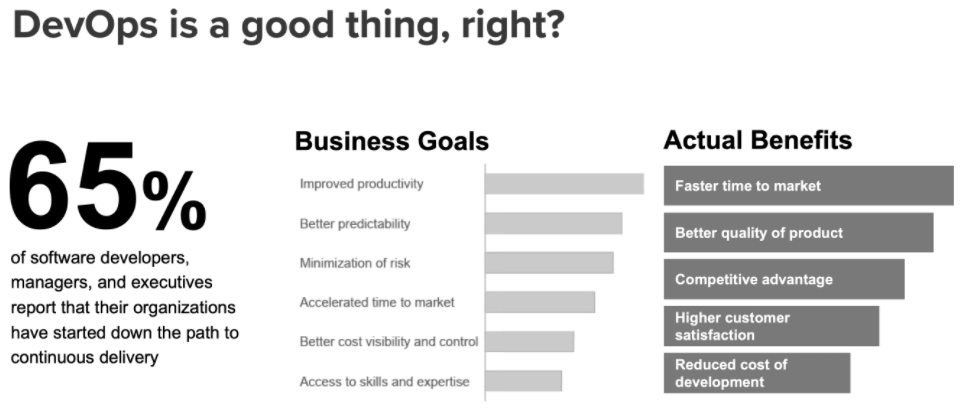
\includegraphics[width=0.9\linewidth]{Cap1/Figura1.png}
\caption{DevOps nas empresas (Fonte: Webinar -- Using VSM to Optimize DevOps Workflow)}
\label{Fig:Fig1}
\end{figure}

%-----------------------------------------------------------------------------------------------------------------
\subsection{A cultura de DevOps}

\hspace{1cm}O movimento DevOps, os seus princípios e práticas podem ser definidos de várias formas. Certos autores, como é o caso de \shortciteA{ebert2016devops}, definem este conceito através de uma visão romântica, quase utópica: \textit{``DevOps é desenvolvimento flexível e rápido, fornecendo processos de negócio. Integra eficientemente o desenvolvimento, a entrega e as operações, traduzindo-se numa ligação elegante e fluída destes três SILOS tradicionalmente separados''}. Outros autores, como \shortciteA{bass2015devops}, descrevem este conceito através de uma visão racional, focada no propósito afirmando que: \textit{``DevOps é um conjunto de práticas que têm como objetivo reduzir o tempo entre a implementação de uma mudança no sistema e a colocação dessa mesma mudança em produção normal, preservando elevada qualidade''}. Tem-se ainda, segundo o autor \shortciteA{huttermann2012devops} uma definição do conceito de DevOps mais prática e equilibrada, vejamos: \textit{``O Termo DevOps é uma mistura de desenvolvimento (representando os software developers, incluindo programadores, testers e técnicos de quality assurance) e operações (representando os peritos que colocam o software em produção, incluíndo os administradores de sistemas, administradores de bases de dados e os técnicos de redes). DevOps descreve práticas que agilizam o processo de entrega de software, realçando a aprendizagem transmitindo feedback, desde a produção ao desenvolvimento, melhorando o tempo do ciclo''}.

\hspace{1cm}Com os devidos pressupostos, cada uma das explicações dadas acerca deste conceito podem ser consideradas como corretas. Isto acontece porque DevOps envolve várias áreas dentro do desenvolvimento (\textit{Dev}) e operações (\textit{Ops}). Faz-se menção à lógica de negócio, às camadas de apresentação -- \textit{back-end} e \textit{front-end} -- passando ainda pela segurança do sistema.  Segundo o autor \shortciteA{startingscaling}, o que se pode afirmar com toda a certeza, é que \textit{DevOps} deve ser definido pelos resultados. De forma a que fique claro, \textit{DevOps} pode ser definido pelo conjunto de normas culturais e práticas tecnológicas que conferem aos projetos um fluxo rápido de trabalho planeado desde -- entre outras fases -- o desenvolvimento através dos testes até às operações, enquanto é preservada confiabilidade, operação e segurança de classe mundial.\\

%-----------------------------------------------------------------------------------------------------------------
\section{\textit{Izilabs Software}}

\hspace{1cm}A \textit{Izilabs Software} é uma empresa com base tecnológica localizada no \textit{REGIA DOURO PARK}, em Vila Real. A empresa foca-se no desenvolvimento de aplicações web, aplicações móveis e de \textit{desktop}, contabilizando vários projetos bem sucedidos, com mais de 5 milhões de downloads e mais de 35 milhões de sessões de utilizadores em todo o mundo, nos últimos anos.

\hspace{1cm}A história da \textit{Izilabs Software} começou em 2010, quando o seu \textit{CEO} Andreas Vilela, ainda estudante, desenvolveu um jogo para \textit{Windows phone}, chamado ``Kill the Duck'', que ficou classificado em segundo lugar na lista de transferências da loja de aplicações, tornando-se no melhor ranking alguma vez obtido por uma aplicação desenvolvida por estudantes. O jogo contabiliza mais de 1.5 milhões de downloads desde 2010.

\hspace{1cm}Em 2012, o Andreas Vilela estabeleceu uma parceria com a Microsoft Portugal com o objetivo de publicar uma aplicação para \textit{Windows 8} na \textit{Windows PC Store}, chamado ``Background Wallpapers HD''. Este aplicativo está presente na lista das melhores aplicações grátis desde 2012, conta com mais de 5 milhões de downloads e aproximadamente 250 000 utilizadores mensais ativos desde a última leitura. A marca \textit{Izilabs Software} foi protegida em 2012 e foram desenvolvidas mais 10 aplicações móveis.

\hspace{1cm}Mais tarde, em 2015, a \textit{Izilabs Software} foi convidada para colaborar no desenvolvimento do ``MB WAY''. Esta aplicação móvel de pagamento permite que os utilizadores façam pagamentos e transferências através da utilização dos seus números telefónicos, que estão associados às suas contas bancárias.

\hspace{1cm}Enquanto que as experiências e projetos da \textit{Izilabs} foram relacionados com soluções B2C (business to consumer), a empresa decidiu entrar no mercado das soluções B2B. No começo do ano de 2016, o Fernando Novais foi convidado como membro do \textit{REGIA DOURO PARK} para conhecer o Andreas Vilela e, em conjunto, formaram um novo projeto (\textbf{Yugoup} -- Let's grow up! -- \textit{Digital marketing plaftorm}).

\subsection{\textit{Yugoup} -- \textit{spinoff}}

\hspace{1cm}A plataforma \textbf{Yugoup} tem como missão trazer as \textit{SME -- Small and Medium Enterprises} para o mundo digital, tornando o marketing digital acessível a todas as organizações. A plataforma conta com seis principais áreas: \textit{Web}, \textit{Mobile Apps}, \textit{E-Commerce}, \textit{Digital Marketing}, \textit{Social Networking} e \textit{Media}.

\hspace{1cm}A plataforma \textbf{} foi construída para considerar os seguintes atributos: Combate à iliteracia tecnológica, Simplicidade, Automatização, Serviço universal, Integração, \textit{User Friendliness}, Dinamismo, Economia digital, Comércio.


%-----------------------------------------------------------------------------------------------------------------
\section{Motivação e Objetivos}
%-----------------------------------------------------------------------------------------------------------------
\hspace{1cm}Este estágio vai consistir na construção do protótipo de uma \textit{pipeline} de integração e entrega contínua de forma a permitir avaliar as vantagens de uma implementação deste tipo tendo em vista a comparação com o processo atual de desenvolvimento de software da empresa.

\hspace{1cm}A introdução de \textit{pipelines} de integração e entrega contínua no desenvolvimento de software requer investigação prévia e realizada de forma periódica. Os autores \shortciteA{eddy2017pilot}, provaram que a curva de aprendizagem deste tipo de ferramentas depende muito do grau de conhecimento que cada um possui. Assim sendo, o primeiro objetivo será compreender -- através de uma pesquisa alargada -- resumir e criar uma base de conhecimento que permita dotar todos os \textit{developers} sobre o comportamento das \textit{pipelines, DevOps, e CI/CD}.

\hspace{1cm}Na fase de construção do protótipo, durante o desenvolvimento dos processos que vão compôr a \textit{pipeline}, é necessário ter em atenção o contexto das políticas da empresa. Portanto, os segundos e terceiro objetivos são: assegurar que a \textit{pipeline} de testes está sob monitorização permanente e garantir que o \textit{output} do resultado da \textit{pipeline} é útil para a empresa em termos de informação apresentada aos \textit{developers}.

\hspace{1cm}Em termos de \textit{feedback}, \shortciteA{dunne2015social} provaram que os defeitos com menos impacto nas aplicações são, na maioria dos casos, encontrados pelos utilizadores. Por outras palavras, pode existir a necessidade de se optar por desenvolver um mecanismo de feedback retroativo entre clientes e a equipa de desenvolvimento. Contudo, não parece ser esse o caso. Para uma empresa que tem como objetivo reportar \textit{code smells}, \textit{bugs} e vulnerabilidades no sistema (para que possam ser rapidamente identificadas e resolvidas) vai ser feita análise estática, vão ser executados testes unitários e testes de integração e performance para mitigar a probabilidade de ocorrerem falhas no sistema. Posteriormente será criada e publicada uma versão funcional da aplicação à qual serão adicionados um conjunto de serviços, desde serviços de bases de dados até a serviços de \textit{load balancing}.


%-----------------------------------------------------------------------------------------------------------------
\section{Organização do Documento}
%-----------------------------------------------------------------------------------------------------------------

\hspace{1cm}Este documento é composto por cinco capítulos e foi escrito tendo em vista a produção de mais um bloco documentado de apoio para os colaboradores da \textit{Izilabs}. É uma base de documentação do processo de desenvolvimento, integração e entrega contínua de um serviço da plataforma, pretende aumentar o conhecimento em temas como \textit{DevOps} e orquestração de micro-serviços tendo como objetivo  providenciar uma nova visão e um conjunto de técnicas passíveis de serem aplicadas a novos projetos. No presente capítulo, foi apresentado o contexto e o enquadramento deste documento, a empresa onde o estágio será realizado, seguido pela motivação, pelas contribuições e pelos objetivos para o desenrolar do estágio.

\hspace{1cm}No segundo capítulo é feito um levantamento ao estado da arte em três domínios, o domínio comportamental, o domínio das práticas correntes e o domínio das tecnologias utilizadas. São apresentados os conceitos-chave sobre os quais o trabalho será fundamentado e são analisados os pontos críticos do estado da arte. Neste capítulo é ainda introduzida a teoria de \textit{pipelines}, é feita uma breve introdução a cada um dos componentes utilizados na configuração da pipeline e é apresentada uma alternativa para cada um dos componentes, uma vez que o foco é a configuração e a construção da \textit{pipeline}. 

\hspace{1cm}No terceiro capítulo é apresentado um estudo de viabilidade das \textit{frameworks} de teste. São apresentadas as tecnologias utilizadas para realizar o estudo, são apresentadas as metodologias de organização e estruturação dos testes e é medido o tempo de execução para cada uma das \textit{frameworks} utilizadas. Em seguida é configurada a \textit{pipeline} de integração e entrega contínua. É abordado o desenvolvimento dos testes unitários em termos de funcionamento, estrutura e processos de validação. Por fim é apresentado um modelo de \textbf{Web API}, que será publicado após a construção de uma versão de \textit{Release}.

\hspace{1cm}O quarto capítulo está dividido em três fases, começando pelo o serviço de gestão de tarefas seguido pela aplicação da \textit{pipeline} a um serviço da empresa e terminando com a integração de um sistema de visualização no ciclo de desenvolvimento. Na primeira fase é apresentada a arquitetura base do serviço e é criada uma imagem com todos os componentes necessários para o funcionamento da aplicação. Depois é composto um ficheiro com todos os serviços que a aplicação necessita e são analisados os pontos críticos deste tipo de metodologia de publicação. Na fase seguinte é criado um \textit{job} para análise de um serviço componente da plataforma \textbf{Yugoup}. É abordada a questão de desenvolvimento de testes de integração e performance que, de seguida, são incluídos na \textit{pipline} juntamente com análise estática e os testes unitários já existentes. Ainda na segunda fase, é criada uma imagem da \textbf{Web API} do serviço que a empresa disponibilizou, são apresentados o \textit{output} da \textit{pipeline}, os resultados e os pontos críticos. Na última fase é apresentado um guia para a integração de um sistema de visualização no ciclo de desenvolvimento e teste de software em desenvolvimento \textit{Agile}. Aqui é explicada a sua utilidade, são apresentados os seus objetivos e, por fim, é discutida a sua otimização.

\hspace{1cm}Por fim, no último capitulo, são tiradas as conclusões sobre o impacto global do estágio, sobre o trabalho desenvolvido na empresa e sobre os principais fatores associados à redução do \textit{time-to-market}. São tecidas algumas recomendações relativamente à implementação do processo na empresa e, neste capítulo, são também apresentados alguns caminhos futuros sobre como é que a empresa pode continuar, a partir deste trabalho, a aumentar a qualidade do seu processo de desenvolvimento de software.

%-----------------------------------------------------------------------------------------------------------------

%-----------------------------------------------------------------------------------------------------------------
%-----------------------------------------------------------------------------------------------------------------
\chapter{Estado da Arte}
\label{Ch:EstadoDaArte}
%-------------------------------------------------------------------------------------------------------------
% Last edited here
\hspace{1cm}Nas \textit{small and medium enterprises} (SME) do setor das Tecnologias da informação (IT), uma alteração ao software nas fases tardias de desenvolvimento é uma aposta que -- no cenário mais pessimista -- pode colocar tudo em jogo. Tendo em conta que as SME são a espinha dorsal da economia Europeia, surge um desafio do seu lado para dar resposta às necessidades dos consumidores de forma rápida e conectada \cite{dunne2015social}. É necessário apresentar uma solução de melhoria contínua para o típico consumidor que está a amadurecer tecnologicamente e exige cada vez mais qualidade dos serviços e produtos que consome.

\section{Hábitos comportamentais}

\hspace{1cm}Quando se produz software, para dar resposta aos requisitos dos clientes, os longos períodos de espera entre \textit{releases} são um risco que pode levar à perda de quota de mercado. A recolha e análise de feedback em tempo útil, sobre se o software -- em desenvolvimento -- vai de encontro aos requisitos de grandes números de utilizadores, é praticamente impossível. Com a introdução de metodologias \textit{Agile}, o software a ser desenvolvido vai sendo testado muito mais cedo no processo de desenvolvimento pelo cliente final e assim é possível analisar o seu comportamento e recolher feedback sobre a sua adequação em termos de solução. Assim sendo, a redução do \textit{time-to-market} e dos \textit{feedback-loops} vai permitir diminuir a discrepância entre aquilo que os \textit{Product Owners} (PO's), \textit{developers} e utilizadores entendem como boas ou más propostas de valor  \cite{raud2016caseStudy}. Evidentemente, nenhuma organização, \textit{developer} ou cliente quer investir tempo e recursos financeiros no desenvolvimento do produto errado. Para além disso, é reconhecido pela indústria de software que os ciclos de \textit{releases} podem ser períodos tensos e frustrantes. Estes sentimentos são conduzidos pelo risco de ocorrerem falhas associadas ao processo de publicação de software para produção. Em projetos de software onde as \textit{releases} são processos manuais intensivos, os ambientes que albergam o software são construídos individualmente, normalmente pelas equipas de operações sendo que, em muitos casos, a equipa de desenvolvimento também intervém nos processos de \textit{deployment}. O software de terceiros que a aplicação necessita para funcionar é instalado, os artefactos das aplicações são copiados para o(s) ambiente(s) de produção e a informação sobre a configuração é copiada ou criada através da consola de administração dos \textit{web servers}, \textit{application servers} ou componentes isolados que integram o sistema. Só depois, os dados das referências são copiados e, finalmente, a aplicação é executada serviço a serviço, componente a componente. Os sentimentos de tensão e nervosismo estão presentes por razões claras. Citando os autores \shortciteA{farley2010contdel}: \textit{``Muitas fases podem correr mal neste processo. Se cada um dos passos não for executado de forma perfeita, a aplicação não vai ser executada corretamente. E, neste ponto, pode não ser claro -- de todo -- qual é o erro, ou qual foi o passo que falhou.''}

\hspace{1cm}Esta é a principal razão pela qual, com o decorrer do tempo, os \textit{deployments} devem tender para ser o mais automatizados possível, não só pela redução do tempo ocupado pelo processo, mas também pelo aumento da resiliência do sistema e pela sucessiva eliminação de falhas provocadas pelo fator humano. Quando não são totalmente ou maioritariamente automatizados, os erros podem (potencialmente) ocorrer sempre que um \textit{deploy} manual for feito. A solução não passa só por perceber se os erros são ou não significantes. Mesmo com excelentes testes de \textit{deployment} os bugs podem ser difíceis de encontrar. Quando os \textit{deployments} não são automáticos o risco de falha aumenta e perde-se a capacidade de serem repetidos de maneira exata -- que leva a desperdícios de tempo -- e, em alguns casos, resulta na impossibilidade de identificar o problema por se desconhecer o processo exato. Um \textit{deployment} manual é uma tarefa complexa, que consome imenso tempo e envolve a colaboração de várias pessoas. É natural que, a cada passo, a documentação criada esteja incompleta ou desatualizada. Por outro lado, em \textit{deploys} automáticos, os \textit{scripts} desenvolvidos podem servir de documentação e vão estar sempre o mais atualizados possível. Se fosse de outra forma, o \textit{deployment} não iria ser concluído com sucesso \cite{farley2010contdel}. 

\section{Práticas correntes}

\hspace{1cm}Ainda de acordo com os autores \shortciteA{farley2010contdel}, integração contínua (CI -- \textit{continous integration}) permite-nos manter a aplicação funcional depois de iteração de novo código e o seu complemento, entrega contínua (CD -- \textit{continuous delivery/deployment}) dá-nos a possibilidade de lançarmos versões novas e funcionais do software, várias vezes por dia. Isto significa que o código produzido e colocado no repositório -- no \textit{branch} principal -- está com qualidade para permitir que as aplicações sejam entregues em qualquer instante. Uma \textit{delivery pipeline} (DP) compreende tanto \textit{continuous integration} de código -- numa primeira fase -- como \textit{continuous delivery} e \textit{deployment} de software para ambientes de teste ou de produção.

\subsection{Integração Contínua}

\hspace{1cm}Uma das primeiras propostas de integração contínua foi feita por \shortciteA{beck2000extreme} como uma das muitas práticas integrantes de \textit{Extreme Programming} (http://www.extremeprogramming.org/). Integração contínua é o primeiro passo na implementação de uma DP e, apesar de não depender do tamanho da equipa de desenvolvimento de software, torna-se especialmente útil com o aumento do número de \textit{developers} a colaborar em conjunto. O objetivo desta mudança é a união de todos os códigos produzidos por eles, existindo um ponto central com o código final e a garantia de que estes módulos se integram devidamente. Com a existência deste ponto central, com o código completo, é possível a implementação de processos automáticos que permitam validar desde processos básicos, como se o código é compilável sem erros, até a processos mais avançados, como testar se o código em si funciona como é esperado. Os resultados destes processos podem permitir ou impedir que o processo continue para fase seguinte. É dada prioridade às \textit{builds} bem sucedidas e ao desenvolvimento de forma que nos permita integrar código sem quebrar o fluxo, ou seja, é recomendado que cada \textit{developer} valide previamente o processo de junção do código antes de o partilhar com os restantes colegas, de forma a evitar que estes fiquem impedidos de trabalhar devido a falhas existentes. Esta mudança é um desafio cultural para equipas de desenvolvimento habituadas a métodos tradicionais. Segundo \shortciteA{startingscaling}: \textit{``Até ser feito, não se consegue imaginar que alguma vez vá funcionar mas, assim que é feito desta forma, não se imagina trabalhar de outra forma. O desafio é assegurarmo-nos que as mudanças culturais ocorrem e que as equipas estão a abraçar esta nova forma de trabalhar.''}

\hspace{1cm}Esta é uma prática que requer que os \textit{developers} façam partilhas (\textit{commit}) dos seus códigos para um sistema de controlo de versões (VCS) pelo menos uma vez por dia, como os autores \shortciteA{fowler2006continuous} sugerem. Depois do \textit{commit} das mudanças no \textbf{VCS}, um orquestrador de processos inicia a \textit{pipeline} de integração contínua para integrar as mudanças do código recebido com o resto do código, é disparado um \textit{trigger} e é feita uma \textit{build} que executa análise estática primeiro, para depois compilar e executar todos os testes unitários disponíveis \cite{raud2016caseStudy}. Um exemplo de uma \textit{pipeline} de integração e entrega contínua (CI/CD) pode ser visto na figura \ref{Fig:Fig2}. 

\hspace{1cm}Se, em qualquer fase da \textit{pipeline}, existir uma falha durante o processo de \textit{build} o seu estado é considerado como \textit{failed}. Em todo o caso, o \textit{developer} é informado acerca do resultado, quer através de feedback sob forma de notificação nos canais de comunicação da empresa (Slack/SMS, ou e-mail para notificações em tempo real), quer através do sistema de visualização integrado no processo de desenvolvimento. 

\begin{figure}
\centering
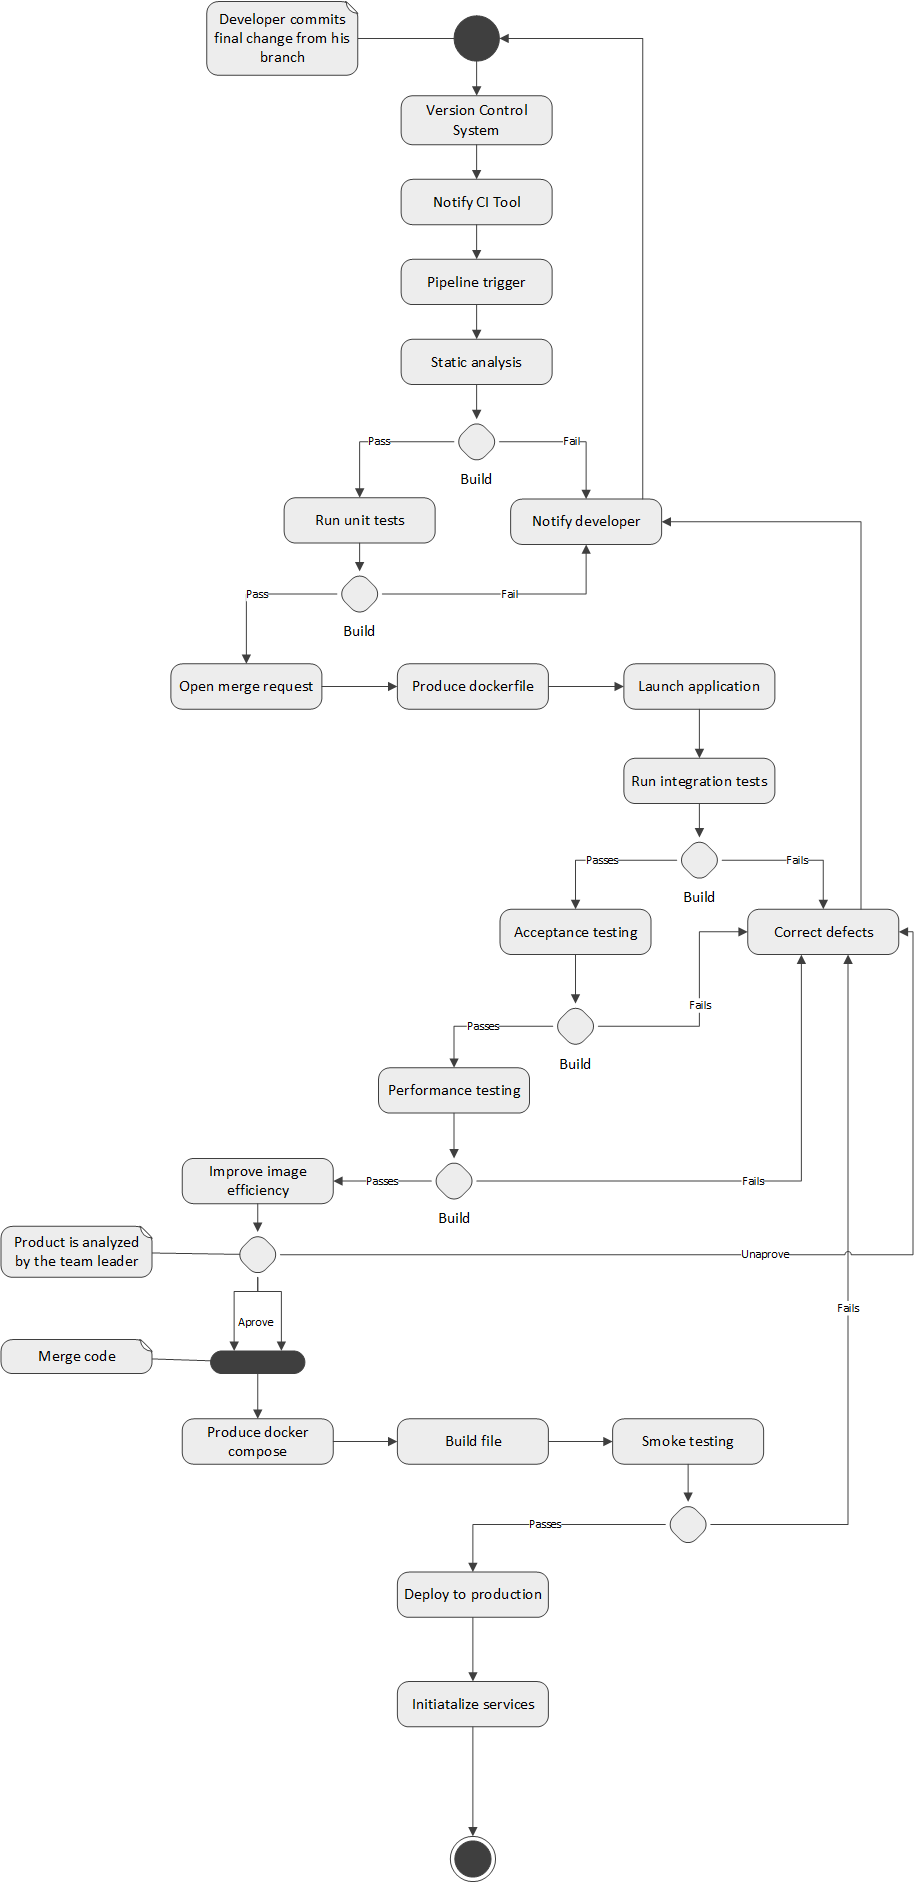
\includegraphics[width=0.7\linewidth]{Cap2/Pipeline_Workflow_UML.png}
\label{Fig:Fig2}
\end{figure}

\hspace{1cm}Quando existe mais do que um \textit{developer}, ou naqueles casos em que se está a desenvolver uma aplicação modular, a possibilidade de introdução de \textit{branches} -- uma espécie de réplica da linha principal -- permite que seja realizado desenvolvimento de uma determinada funcionalidade de forma independente e facilita que o código seja depois unido à linha principal sem que outros programadores sejam forçados a aguardar a sua conclusão \cite{farley2010contdel}.

\hspace{1cm}Fundamentalmente, a integração contínua exige a capacidade de manter a aplicação funcional depois de iterar novo código. Por forma a aumentar a qualidade do desenvolvimento do software, existem algumas abordagens ao desenvolvimento que podem ser úteis para aumentar a qualidade do produto final. Uma delas é o Desenvolvimento Orientado a Testes (\textit{TDD -- Test Driven Development}) proposto por \shortciteA{BeckTDD2002}, que propõe o desenvolvimento orientado a testes como sendo a ideia de que, quando estamos a desenvolver novas funcionalidades ou corrigimos erros, os \textit{developers} criam primeiro um teste que é uma especificação executável para o comportamento esperado do código a ser escrito. Estes testes motivam o \textit{design} das aplicações servindo de testes de regressão e, simultâneamente, de documentação de código e do comportamento esperado da aplicação \cite{farley2010contdel}.

\subsection{Entrega Contínua}

\hspace{1cm}Entrega contínua exige que sejamos capazes de fazer \textit{deploys} da aplicação a qualquer momento tanto para ambientes de teste como para ambientes de produção \cite{farley2010contdel}. Uma das técnicas chave para mantermos as aplicações publicáveis a qualquer instante -- mesmo apesar das mudanças constantes -- é a modelação dos componentes da aplicação e utilização de interfaces de comunicação. Imagine-se um componente como um grande bloco de código dentro de uma aplicação (com uma Web API bem documentada) que pode eventualmente ser trocada por outra implementação desde que respeite a interface definida. Um sistema de software baseado em componentes é distinguido pelo facto de que a sua base de código está dividida em pedaços discretos que providenciam comportamento sob forma de interações limitadas, através dessas interfaces bem definidas, com outros componentes \cite{farley2010contdel}.

\hspace{1cm}A utilização de \textit{pipelines} de integração contínua em produção e desenvolvimento de software, pode poupar muitas horas de trabalho. Partindo do  código-fonte no \textbf{VCS}, construir a aplicação, executar análise estática, testes unitários, empacotar e publicar a aplicação para um repositório remoto, são processos que consomem algum tempo. Este tempo aumenta com a complexidade e tamanho da aplicação e, por vezes, é tempo que podia ser investido no desenvolvimento de uma funcionalidade em vez de desperdiçado na execução repetitiva de um conjunto de instruções. 

\hspace{1cm}De qualquer das formas, a automatização deste processo deve ser planeada de acordo com o tamanho e modularidade de cada aplicação. Para aplicações mais complexas, podem ser necessárias várias imagens para que a aplicação seja executada. Podem existir inúmeros \textit{deployments} em múltiplos locais -- dependendo da quantidade de fases existentes -- e pode ser necessário ajustar o número de \textit{deployments} dependendo da infraestrutura que a organização tem ao seu dispor.

\hspace{1cm}Imagine-se um contexto em que um projeto exige a integração de código de cinco \textit{developers} diferentes, sendo cada um responsável por funções diferentes dentro da \textit{stack} de tecnologias a usar (BD, backend, frontend, etc). Se o \textit{Product Owner} dá preferência à utilização das práticas de \textit{DevOps} com o projeto em fase final, o projeto vai precisar não só de um ajuste em termos de estrutura organizacional, mas também de uma revisão geral de todos os processos. Neste caso em particular, a equipa está a desenvolver uma plataforma de \textit{e-commerce} e as várias arquiteturas do sistema estão fechadas, sendo apenas necessárias pequenas correções em alguns serviços que a compõem. Aqui, evidentemente, dado o grau de complexidade do sistema em desenvolvimento e o tempo investido na sua modelação -- não só em termos macro (plataforma), como também em termos micro (serviços) -- é mais vantajoso manter as práticas correntes e continuar com o mesmo método de trabalho. Nem sequer se coloca em cima da mesa outro conjunto de fatores como por exemplo a barreira cultural da resistência à mudança. O projeto iria precisar de uma revisão geral tão extensa que todo o tempo de todos os integrantes da equipa teria de ser investido na revisão de metodologias de trabalho. Isto representaria largos períodos de tempo que, obviamente, são cruciais para a finalização dos serviços que compõem a plataforma no imediato e que não podem sequer ser considerados em termos monetários.

\hspace{1cm}Noutro contexto, dispõe-se exatamente da mesma equipa de \textit{developers} a trabalhar no desenvolvimento de uma aplicação web de submissão de currículos. E um dos requisitos do \textit{business}, com o projeto em fase de arranque, indica que o desenvolvimento será feito mediante as práticas da cultura \textit{DevOps}. Neste caso, a equipa não tem qualquer tipo de ideia de qual será o alinhamento -- em termos de arquitetura -- do sistema. Aqui, contrariamente ao exemplo anterior, não tendo ainda sido investido tempo na modelação do sistema nem no seu planeamento, faz sentido a adoção das práticas de \textit{DevOps} uma vez que a mudança na cultura de trabalho será feita a partir do começo do projeto, abrindo-se espaço a um processo gradual de adaptação.

\hspace{1cm}A cultura \textit{DevOps} é portanto um complemento fundamental ao desenvolvimento \textit{Agile} e os benefícios das suas práticas são promissores. A implementação deste tipo de práticas traz imensas vantagens para o desenvolvimento de software em equipa. Em contrapartida, quanto mais tardia for a mudança para este conjunto de normas ou práticas diárias, mais difícil será a adaptação. A filosofia \textit{Agile}, por si só, é muita das vezes considerada insuficiente ou ineficaz na gestão de projetos de desenvolvimento de software. Daí ser comum encontrar outros conjuntos de técnicas e estratégias de gestão aliados a esta filosofia, como é o caso do \textit{Scrum} (https://www.atlassian.com/agile/scrum) para gestão do trabalho de vários elementos e do \textit{Kanban} (https://www.atlassian.com/agile/kanban) para representação visual do fluxo de trabalho.

\hspace{1cm}Considerando que as metodologias de gestão e planeamento devem contabilizar vários fatores internos e externos à equipa responsável pela execução do projeto, desde as políticas da internas da empresa até ao contexto do negócio, é importante ter em conta que a produção deste protótipo tem como objetivo ir de encontro à prestação de serviços \textit{business-to-business} (B2B).

\hspace{1cm}Naquilo que à prestação de serviços diz respeito, é o \textit{Information Technology Infrastructure Libary} (ITIL) conhecido como um dos conjuntos detalhados de boas práticas que se concentra no alinhamento de serviços de IT com as necessidades dos negócios. Resumidamente, o \textbf{ITIL} baseia-se em quatro disciplinas -- \textit{service request}, \textit{incident}, \textit{change} e \textit{problem}.

\hspace{1cm}O \textbf{ITIL} atua sobre três pontos cruciais de \textit{IT Service Management} (ITSM). São eles os processos, a comunicação e a transparência. Este conjunto de práticas \textit{post-deployment} atua sobre \textbf{processos} pouco (ou nada) definidos e implementados com as ferramentas erradas. Atua sobre \textbf{comunicação}, em equipas que trabalham de forma isolada, que não se focam na comunicação fora do deu \textit{SILO} e atua sobre a \textbf{transparência} onde as equipas de clientes ou de parceiros nem sempre têm visibilidade dos itens de trabalho ou dos processos pertinentes.

\hspace{1cm}Apesar de ser pouco comum a comparação entre filosofias e \textit{frameworks} -- como é o caso do \textit{Agile} em contraposição com o \textbf{ITIL} -- pode ser útil aliar uma filosofia, diga-se, anárquica a um conjunto de boas práticas bem definido, com atenção ao detalhe e com definição concreta no que diz respeito ao processo. Portanto, aliar estes dois pólos opostos e aplicar \textbf{ITIL} em processos cirúrgicos para estruturação das metodologias de trabalho pode ser vantajoso para tirar partido dos seus pontos fortes. Nos aspetos em que a filosofia \textit{Agile} sái mais fragilizada pode eventualmente ser aplicado o \textbf{ITIL} para nutrir os processos com resiliência e para providenciar bases sólidas, bem documentadas, em melhoria contínua do serviço \cite{axelositilandagile}.   
%-----------------------------------------------------------------------------------------------------------------
%\chapter[Teoria das \textit{pipelines}]{Teoria das \textit{pipelines}}
\section{Tecnologias utilizadas}
\label{Ch:TeoriaDasPipes}

\hspace{1cm}A técnica de \textit{pipelining} é muitas vezes comparada a uma linha de montagem industrial onde são produzidos vários tipos de componentes ao mesmo tempo, dentro de uma sequência lógica de acontecimentos, para um determinado processo produtivo. Mesmo existindo uma certa dependência em termos sequenciais, no global, o processo tira vantagem de operações que acontecem em paralelo.

\hspace{1cm}O conceito de \textit{pipelining} em engenharia informática advém de arquitetura de computadores. Consiste numa técnica de decomposição de processos sequenciais de controlo em subprocessos, sendo que cada um desses subprocessos é executado num segmento especialmente dedicado que opera concorrentemente com os outros segmentos. 

\hspace{1cm}As primeiras aplicações práticas de \textit{pipelining} em arquitetura de computadores surgiram no início da década de 80 e foram avanços extraordinários para a indústria de processamento digital de informação. Este tipo de arquitetura flexível -- baseada em operações paralelas -- foi adaptada aos requisitos funcionais de um conjunto de modelos de computadores, o que permitiu aumentar gradualmente a capacidade de processamento de informação. Estes avanços foram baseados na adição de novos componentes responsáveis principalmente pelo melhoramento da execução sequencial de instruções e pela mitigação e prevenção de \textit{stack overflows} \cite{potash1984flexible}. Mais próximo do final da década, aliado a outro conceito inovador, surgiu o primeiro computador multi-nó com processamento paralelo reconfigurável. Esta inovação tinha por base a computação feita através de vários nós. Foi impulsionada pelo desenvolvimento de uma topologia em \textit{hypercube} e revolucionou a indústria da computação através da adição de novos componentes aos processadores -- como os \textit{multiplexers}, os \textit{memory-ALU switches} e os mecanismos de \textit{caching} -- que eram orquestrados pelos micro-controladores e pelos micro-sequenciadores \cite{nosenchuck1989multinode}. Para termos uma base de comparação, imaginemos a descoberta dos autores \shortciteA{potash1984flexible} como uma \textit{pipeline} e a descoberta dos autores \shortciteA{nosenchuck1989multinode} como uma \textit{pipeline} de \textit{pipelines}. 

\hspace{1cm}Mais tarde, no início da década de 90, surgiram alguns dos princípios que ainda hoje são aplicados em computação sequencial. Através da administração de um \textit{crossbar switch}, os elementos unitários de processamento e os módulos de memória paralelos passaram a poder ser alterados dinamicamente -- ciclo após ciclo -- de acordo com os requisitos de cada um dos algoritmos em execução. Esta inovação, composta por duas secções -- um \textit{multiplexer} e uma secção de controlo -- trouxe melhorias principalmente para a área do processamento digital de imagem \cite{hiller1992highly}. Depois, através da reintrodução de componentes estáticos aliados aos componentes dinâmicos já existentes, surgiram métodos focados na otimização da performance e na conservação de energia. A introdução dos componentes estáticos era promissora por duas razões. Primeiro permitiria preservar informação que daria ao sistema a capacidade de resumir a execução dos processos mais tarde, depois de um \textit{system clock} ser parado (\textit{halted}), sem que os dados fossem perdidos. Segundo, para além da redução no consumo -- comparativamente com um sistema implementado inteiramente em lógica dinâmica -- também era minimizado o custo de operação, de produção e a área do circuito eletrónico  \cite{donner1993computer}. Ou seja, o processador ficava assim mais pequeno, a sua produção ficava menos dispendiosa e a sua operação mais sustentável.


\subsection{Orquestração da \textit{pipeline}}

\hspace{1cm}A \textit{pipeline} faz orquestração sequencial de análise estática, testes unitários e testes de integração/performance do projeto. Depois é produzida uma imagem da versão executável do projeto que vai ser publicada num registo privado, onde vai ser armazenada. O último passo antes da passagem para produção é a criação de um ficheiro de composição de todos os serviços que a aplicação necessita para ser executada de forma automática através da execução de uma única instrução. Existe um conjunto de ferramentas cuja utilização é comum a todas as fases, como é o caso do \textbf{Jenkins} (orquestrador de processos) e do \textbf{GitLab} (\textbf{VCS}). Dependendo das fases de \textbf{SDLC}, ou \textbf{STLC}, vão ser utilizadas outras ferramentas para análise estática, repositórios de artefactos, ferramentas de virtualização em \textit{containers} e registos privados de imagens.

\subsection{Orquestrador de processos}
\hspace{1cm}Um orquestrador de processos é simultaneamente o coração e o cérebro da \textit{pipeline} de integração e entrega contínua. Faz a automatização \textit{end-to-end} do sistema. Para além puxar para si o código dos repositórios, executa instruções, faz a manutenção do código através da compilação do mesmo e da execução dos testes. No fundo, pode -- dependendo da complexidade das instruções -- desempenhar uma panóplia de funções de automação.

\hspace{1cm}O \textbf{Jenkins} (https://jenkins.io/) é o líder do mercado no que toca a servidores \textit{open-source} de automação de projetos. Focado na automação contínua das \textit{builds} e dos testes dos projetos, o \textbf{Jenkins} acrescenta valor através do aumento da produtividade e da integração dos \textit{logs} de cada \textit{build} na sua \textbf{GUI}. 

\hspace{1cm}Outros serviços de integração contínua, como o \textbf{Travis-CI} (https://travis-ci.com/) e o \textbf{Azure DevOps} (https://azure.microsoft.com/pt-br/services/devops/), requerem a criação de um \textit{script} com todos os passos para definir os processos a ser executados pela \textit{pipeline}. Para além da configuração em forma de \textit{script}, estes serviços de integração contínua requerem um nível de conhecimento e à vontade mais elevados para poderem ser configurados de acordo com os objetivos definidos. Apesar de serem ambos opções viáveis devido à elevada quantidade de informação disponibilizada pela comunidade,  o \textbf{Jenkins} será a ferramenta elegida uma vez que é \textit{open source} e pode ser utilizado para a apresentação da informação dos estados das builds \textit{on the fly}. Comparativamente com outros servidores de automação, como é o caso do \textbf{GitLab CI} (https://docs.gitlab.com/ee/ci/), o \textbf{Jenkins} é das ferramentas de integração contínua cuja informação é mais fácil de encontrar uma vez que era a ferramenta com que a empresa já detinha alguma experiência em termos de utilização. O \textbf{GitLab} foi utilizado como forma de armazenamento na \textit{cloud} do \textbf{VCS}.


\subsection{\textit{Version Control System}}
\hspace{1cm}O sistema de controlo de versões é um sistema que permite armazenar todas as alterações realizadas a um determinado conjunto de ficheiros, e armazenar todas essas alterações num histórico, o que permite voltar atrás caso seja necessário. Esta é uma ferramenta fundamental para os \textit{developers}, pois permite armazenar todas as alterações ao código realizadas não só por um programador, mas por vários. E como o que é armazenado pelo \textbf{VCS} é a diferença entre os ficheiros iniciais e final (delta) -- ou seja, as linhas adicionadas e as linhas removidas -- torna o processo de união dos ficheiros de múltiplos programadores muito mais eficiente e, em muitos casos, quase automático.

\hspace{1cm}O \textbf{GitLab} (https://gitlab.com/) é uma ferramenta de gestão de repositórios de software com suporte a \textit{Wikis}, a gestão de tarefas e a integração e entrega contínua. A empresa utiliza esta ferramenta de gestão de repositórios de software para o armazenamento de praticamente todos os projetos que desenvolve. Isto quer dizer que todo o código que foi desenvolvido durante o período de estágio foi publicado e está armazenado em repositórios \textbf{GitLab}. O \textbf{GitHub} (https://github.com/) é outro bom exemplo de uma ferramenta de gestão de repositórios de software com suporte a \textit{Wikis} e gestão de tarefas, focado na partilha de código e na interação social entre os \textit{developers}. Existem imensos serviços de armazenamento de código na \textit{cloud}, entre os quais se podem destacar o \textbf{Bitbucket} (https://bitbucket.org/), o \textbf{Subversion} (https://subversion.apache.org/), o \textbf{Gogs} (https://gogs.io/) entre outros, dos mais respeitados e conhecidos do mercado. Para este caso, tendo em este contexto empresarial da atual metodologia de desenvolvimento de código, o \textbf{GitLab} foi a ferramenta é utilizada no que diz respeito à componente de armazenamento de código na \textit{cloud} do \textbf{VCS}.

\hspace{1cm}Podemos comunicar com os servidores de formas distintas. Através da utilização de \textit{(https://)}, ou através da utilização de um túnel, o \textit{\textbf{secure shell}} (SSH). Neste caso, para publicarmos o código no repositório, vai ser utilizado o protocolo \textbf{SSH}. 

\hspace{1cm}O protocolo \textbf{SSH} encripta as ligações entre um cliente e um servidor. Encripta todas as mensagens, desde instruções até às credenciais de autenticação do utilizador. Tudo aquilo que é comunicado entre os dois \textit{peers} é encriptado por um par de chaves. Uma chave é pública -- fica sempre do lado do servidor -- e outra chave, que dá acesso ao servidor a quem tiver uma cópia, é privada. Posteriormente, a chave privada será utilizada para que o orquestrador de processos possa puxar o código que publicamos no repositório.  

\subsection{Análise estática}

\hspace{1cm}A análise estática, é uma análise léxica (estrutural) e sintática (declarativa) para identificar más práticas no código desenvolvido ou declarações consideradas perigosas. Quando integrada numa \textit{pipeline} de integração e entrega contínua, a análise ao código é feita de forma 100\% automática garantindo a verificação das duas primeiras camadas da \textbf{stack} enquanto que as verificações semânticas do contexto da funcionalidade são feitas pelos testes unitários. A gravidade dos elementos possivelmente identificados pela análise estática, depende essencialmente de políticas existentes numa determinada organização. Isto quer dizer que duas empresas podem ter interpretações diferentes do mesmo relatório de análise estática.

\hspace{1cm}O \textbf{SonarQube} (https://www.sonarqube.org/) é uma plataforma de gestão dedicada à análise contínua de qualidade do código. Já contém milhares de regras de análise estática de código e é utilizada para analisar várias linguagens. À semelhança desta plataforma, também o \textbf{Codacy} (https://www.codacy.com/) pode ser utilizado para automatizar estes parâmetros das \textit{code reviews} e monitorizar a qualidade do código elaborando relatórios do impacto de cada \textit{commit} ou \textit{pull request}. Apesar de existirem outras ferramentas de análise estática no mercado com as mesmas funcionalidades, é o \textbf{SonarQube} que vai ser utilizado para revisão da qualidade do código uma vez que é facilmente integrável na \textit{pipeline} e pode ser virtualizado em \textit{containers}. 

\subsection{Repositório de artefactos}

\hspace{1cm}O repositório de artefactos é um órgão vital para o funcionamento da \textit{pipeline} de integração e entrega contínua. É lá que são publicados os artefactos que produzimos através da execução do código desenvolvido. Estes componentes, modulares e simples de manter, podem desempenhar uma função específica dentro de \textbf{Web API}, de uma \textbf{Web Application} ou de uma \textbf{console aplication} que se pretenda desenvolver. O repositório utilizado para armazenar artefactos irá ser, mais tarde, reintegrado no ambiente integrado de desenvolvimento (IDE) e é a partir de lá que podem ser descarregados e utilizados os \textit{NuGet packages}.

\hspace{1cm}A \textbf{Sonatype} disponibiliza uma ferramenta grátis para armazenamento de artefactos. O \textbf{Nexus Repository Manager OSS} (https://www.sonatype.com/nexus-repository-oss) é um repositório de artefactos compatível com os formatos de artefactos mais conhecidos. Também foram avaliadas outras hipóteses, como por exemplo o \textbf{JFrog artifactory} (https://jfrog.com/artifactory/) -- um repositório de artefactos com caratetísticas semelhantes ao supra-mencionado \textbf{Nexus} -- o \textbf{Whitesource} (https://www.whitesourcesoftware.com/), o \textbf{ProGet} (https://inedo.com/proget) e o \textbf{MyGet} (https://www.myget.org/), que têm o mesmo tipo de metodologia de armazenamento de artefactos com estratégias de caching. 

\hspace{1cm}Durante as fases de desenvolvimento do protótipo da \textit{pipeline} será utilizado o \textbf{Nexus Repository Manager OSS}. Mais tarde, será utilizado o \textbf{MyGet} para injeção de dependências num contexto ligeiramente diferente. 

\subsection{Orquestração de \textit{containers}}

\hspace{1cm}A orquestração de \textit{containers} é a capacidade de provisionar automaticamente a infraestrutura necessária para atender às necessidades de um projeto, sem a necessidade de utilização de máquinas físicas. Conceptualmente semelhante a máquinas virtuais, mas com o foco em serviço, cada \textit{container} é um serviço em si e apenas um só. Esta abordagem promove a independência dos serviços, aumenta a resiliência do sistema e, principalmente, facilita o desenvolvimento e \textit{deployment} dos serviços em produção. 

\hspace{1cm}O \textbf{Docker} é -- à semelhança do \textbf{rkt} (https://coreos.com/rkt/) -- uma tecnologia de virtualização em \textit{containers}. Segundo o \textbf{\shortciteA{dockercontainers2}}, os \textit{containers} são métodos de \textit{packaging} de aplicações que são executadas, juntamente com as suas dependências, isoladas de outros processos. O \textbf{Docker} funciona através da criação de imagens (\textbf{Dockerfiles}) que posteriormente são executadas em \textit{runtime} dentro de um \textit{container}. Comparativamente com outras ferramentas, como o \textbf{Podman} (https://podman.io/) e o \textbf{Buildah} (https://buildah.io/), que são utilizados para orquestrar \textit{containers} e gerar imagens respetivamente, o \textbf{Docker} pode ser utilizado para estas duas tarefas. Vai ser tirado partido desta vantagem uma vez que, neste contexto, é preferível utilizar a mesma tecnologia tanto na construção de imagens, como na orquestração de \textit{containers}.

\hspace{1cm}Inicialmente, o \textbf{Docker} era uma ferramenta desconhecida cujo conceito foi explorado no decorrer do estágio. À medida que o protótipo foi desenvolvido, a utilidade do \textbf{Docker} na orquestração dos serviços foi ganhando importância. Verificou-se que, no repositório público (https://hub.docker.com/), existiam imagens para serviços de \textbf{VCS}, serviços de bases de dados, de análise estática, de armazenamento de artefactos, armazenamento de imagens e por aí em diante. O que é curioso, é que a grande maioria dos serviços que as organizações utilizam no seu dia-a-dia disponibilizam imagens de \textbf{Docker} para uso da comunidade. Neste repositório conseguimos encontrar imagens de serviços como o \textbf{MS SQL Server}, \textbf{SonarQube}, \textbf{Sonatype Nexus}, \textbf{Docker Registry 2.0} entre outros.

\hspace{1cm}O \textbf{Docker Swarm} (https://docs.docker.com/engine/swarm/) é uma ferramenta nativa do \textbf{Docker} que permite colocar um \textit{cluster} de \textit{containers} em ambiente de teste ou produção e controlar esse mesmo conjunto de \textit{hosts}. O \textbf{Kubernetes} (https://kubernetes.io/) é outro orquestrador de \textit{containers} \textbf{Docker} que permite gerir \textit{workloads} de forma a garantir que o estado dos \textit{clusters} vai de encontro às necessidades dos utilizadores. Através da utilização de dois conceitos \textit{``labels''} e \textit{``pods''}, os \textit{containers} são agrupados em \textit{logical units} para facilitar a sua gestão. Outras tecnologias, como o \textbf{Openshift} (https://www.openshift.com/), podem ser utilizadas para \textit{deployments} em conjunto com o \textbf{Kubernetes} em sistemas operativos como o \textbf{RHEL} ou o \textbf{CentOS}. Estes três mecanismos de orquestração de \textit{containers} podem e devem ser comparados mais tarde, noutro estudo, em termos de custo de execução e de operação aquando dos \textit{deployments} da plataforma para produção.

\subsection{Workflow da pipeline de CI/CD}

\hspace{1cm}Concluído o levantamento do estado da arte, tudo indica que a \textit{pipeline} CI/CD será composta por quatro fases: \textit{development}, \textit{staging}, \textit{pre-live} e \textit{production}.

\subsubsection{\textit{Development Environment}}

\hspace{1cm}Na fase de \textit{development} da \textit{pipeline} (\ref{Fig:Fig3}), um \textit{job} faz \textit{fetch} ao código presente no \textbf{VCS} e, através de um conjunto de instruções, faz \textit{build} à solução, executa análise estática e todos os testes unitários. Durante este processo são interpretados e apresentados os seus resultados.

\hspace{1cm}Pela sequência lógica dos acontecimentos, a fase de \textit{development} deve terminar com um \textit{deployment} para \textit{staging}. Como é possível constatar nos próximos capítulos, podem existir vários cenários de \textit{deployment}. Neste caso serão considerados dois cenários diferentes. Um primeiro cenário onde o objetivo é validar um conjunto de funcionalidades através da execução dos testes unitários em conjunção com a análise estática e um outro cenário onde se pode adicionar \textit{packaging} e \textit{push} desse conjunto de funcionalidades ao \textit{flow}. Apesar de existirem outras possibilidades para o \textit{deploy}, serão trabalhados maioritariamente os dois cenários acima discutidos.

\begin{figure}[hbt!]
\centering
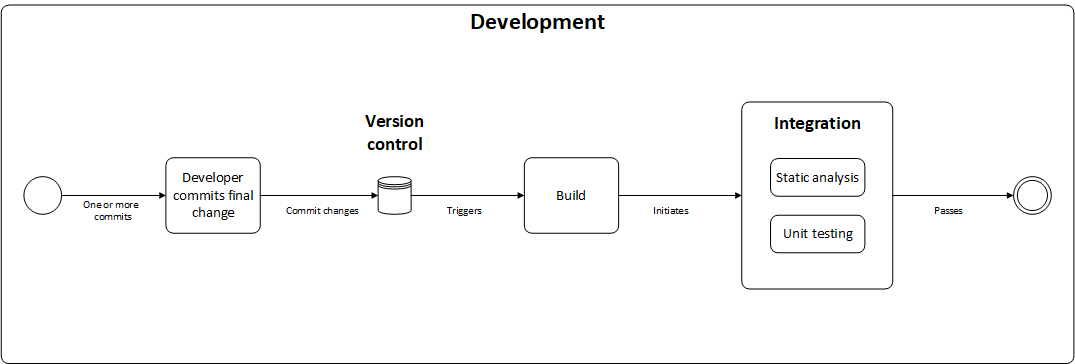
\includegraphics[width=0.8\linewidth]{Cap2/DevelopmentStage.png}
\caption{\textit{Workflow} de um \textit{job} da fase de \textit{development}}
\label{Fig:Fig3}
\end{figure}

\subsubsection{\textit{Staging Environment}}

\hspace{1cm}Na fase de \textit{staging} (\ref{Fig:Fig100}) é produzida uma imagem da aplicação que depois será colocada no repositório privado de imagens. Depois de lançada e validada a aplicação, são feitos testes de integração e performance, a aplicação é validada pelo \textit{product owner} e -- opcionalmente -- pode ser incluída nesta fase uma análise à qualidade de compressão da imagem através da utilização do \textbf{Dive} \cite{dockerdive}.

\begin{figure}[hbt!]
\centering
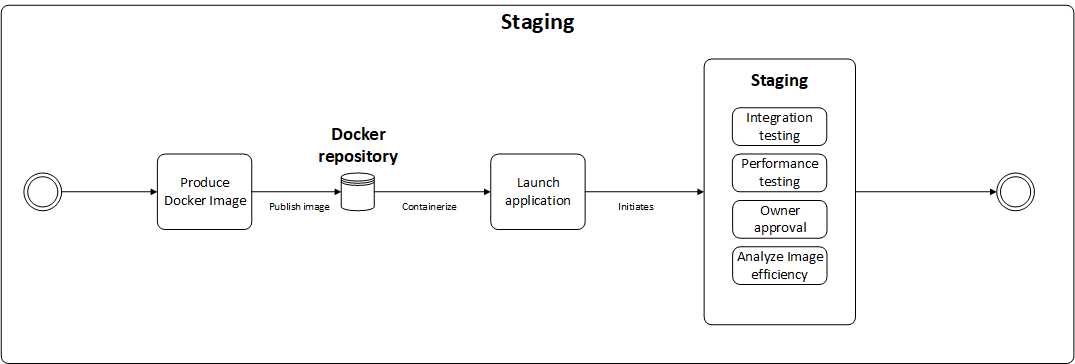
\includegraphics[width=0.8\linewidth]{Cap2/Staging.png}
\caption{\textit{Workflow} de um \textit{job} da fase de \textit{staging}}
\label{Fig:Fig100}
\end{figure}

\hspace{1cm}Faz sentido incluir análise estática nesta fase apesar de não ser obrigatório. A análise estática pode ser utilizada como uma fase extra de verificação ao código da \textbf{Web API} desenvolvida em \textbf{C\#}, uma vez que o código presente em \textbf{VCS} terá de ser validado e aprovado para que o processo de criação da imagem seja automatizado.

\subsubsection{\textit{Pre-live Environment}}

\hspace{1cm}A fase de \textit{pre-live} assemelha-se com um ambiente de produção. O objetivo é precisamente configurar um \textit{job} com um conjuto de processos que simulem a publicação de uma aplicação para produção, juntamente com todos os serviços dos quais a aplicação depende, executar um conjunto de verificações -- nomeadamente validar que o comportamento da aplicação vai de encontro ao esperado -- e submeter a aplicação a uma fase final de aprovação pela mão do \textit{product owner}.

\begin{figure}[hbt!]
\centering
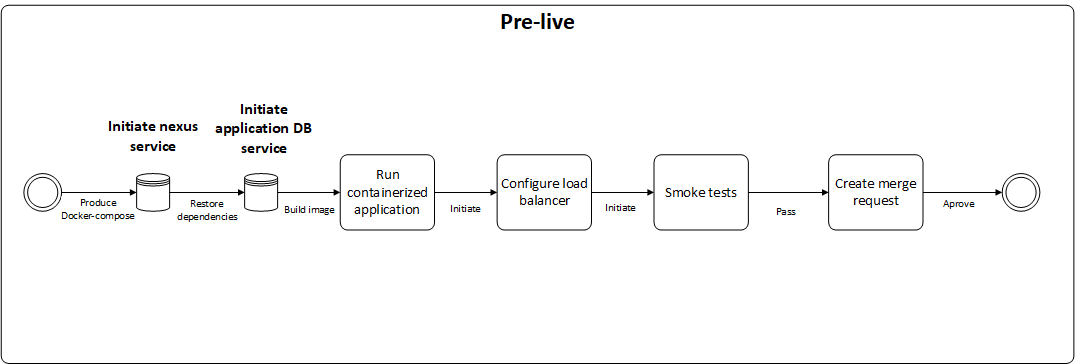
\includegraphics[width=0.8\linewidth]{Cap2/PreLiveStage.png}
\caption{\textit{Workflow} de um \textit{job} da fase de \textit{pre-live}}
\label{Fig:Fig97}
\end{figure}

\hspace{1cm}Como se pode ver pela figura \ref{Fig:Fig97}, a configuração do ambiente começa, à semelhança de uma fase de produção, com a configuração de um documento de composição de todos os serviços (docker-compose.yml) da aplicação. O documento terá de incluir a configuração sequêncial dos serviços por ordem cronológica de acontecimentos, depois são feitos testes à aplicação e opcionalmente pode ser criado um \textit{merge request}.

\subsubsection{\textit{Production Environment}}

\hspace{1cm} A única diferença entre este \textit{job} e o anterior é a remoção dos \textit{tests}, do \textit{merge request} e das validações do \textit{product owner} uma vez que teriam sido feitos anteriormente. Para esta fase pode ser considerada a adição de serviços de monitorização (\ref{Fig:Fig98}) como é o exemplo do \textbf{ELK Stack} (https://www.elastic.co/pt/elk-stack) e do \textbf{Nagios} (https://www.nagios.org/).

\begin{figure}[hbt!]
\centering
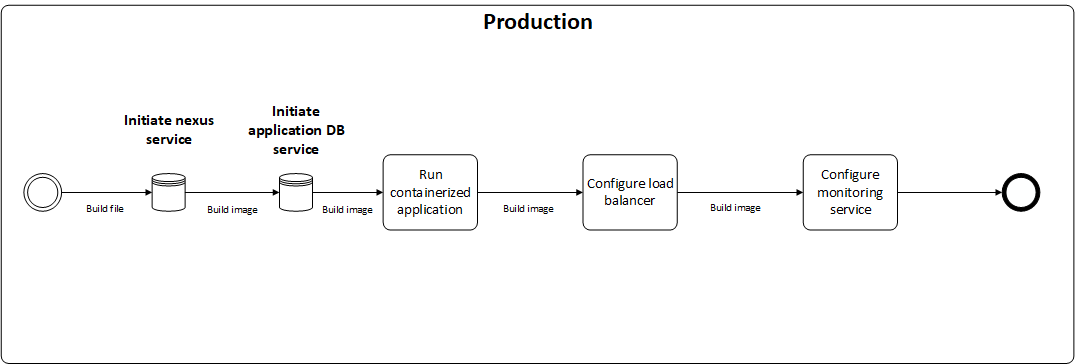
\includegraphics[width=0.8\linewidth]{Cap2/ProductionStage.png}
\caption{\textit{Workflow} de um \textit{job} da fase de \textit{production}}
\label{Fig:Fig98}
\end{figure}

\hspace{1cm}Caso estajamos a considerar a adição destes ou de novos serviços de monitorização na fase de produção é importante ter em mente que todos os serviços devem ser testados e validados previamente durante a fase de \textit{pre-live}. 

\hspace{1cm}É também importante mencionar que estes \textit{jobs}, desenvolvidos para cumprir um conjunto de objetivos pré-estabelecidos num contexto específico, podem não ter o mesmo tipo de resultado quando aplicados a outros contextos de negócio. Ao longo do estágio, durante a construção do protótipo da pipeline, as considerações e as decisões tomadas estiveram de acordo com aquilo que são as necessidades da empresa.
%-----------------------------------------------------------------------------------------------------------------
%\include{Cap3/CAP3} Passou para o 5
%-----------------------------------------------------------------------------------------------------------------
%\include{Cap4/CAP4}
%-----------------------------------------------------------------------------------------------------------------
%-----------------------------------------------------------------------------------------------------------------
\chapter[Construção da \textit{pipeline} de integração contínua]{Construção da \textit{pipeline} de integração contínua}
\label{Ch:CapExemplo}
%-----------------------------------------------------------------------------------------------------------------
\section{Estudo de viabilidade das \textit{frameworks} de teste}
\label{Ch:OutroCap}

\hspace{1cm}Uma das vantagens da implementação de uma \textit{pipeline} de testes automatizada é a redução do tempo de validação e entrega de código funcional. Para que o código esteja funcional é necessário que, em primeiro lugar, corresponda aos requisitos para o qual está a ser desenvolvido. Uma vez verificada a funcionalidade -- e tendo sido verificado que os seus requisitos estão de acordo com as expectativas iniciais -- podemos então pensar no segundo ponto que consiste na otimização da \textit{pipeline}, isto é, na redução da duração do tempo de compilação dos projetos, dos testes e de outros processos. Sabendo que existem várias \textit{frameworks} à disposição, dependendo da linguagem de programação utilizada para desenvolvimento, foram escolhidas aquelas que se melhor se ajustam ao contexto da execução dos testes.


\hspace{1cm}No desenvolvimento orientado a testes há uma metodologia de organização e estruturação do código bastante interessante, que é dividida em três fases: \textit{Arrange, Act} e \textit{Assert}. Esta abordagem aos testes é conhecida no mundo da programação como AAA ou \textit{triple A}.

\subsection{\textit{Arrange, Act \& Assert}}

\hspace{1cm}Na primeira fase, \textbf{\textit{Arrange}}, apenas temos o código necessário para o \textit{setup} daquele \textit{test case}. É aqui que são criados os objetos ou \textit{mocks} (caso existam) e também é nesta fase que é definido o resultado esperado. Na segunda fase, \textbf{\textit{Act}}, é onde normalmente são invocados os métodos que vão ser testados. Na última fase, \textbf{\textit{Assert}}, vai ser verificado se o resultado obtido na execução das duas fases anteriores vai de encontro ao resultado esperado. Na figura \ref{Fig:Fig7} encontra-se um exemplo de uma classe de teste desenvolvida em \textbf{MSTest}. Esta classe de teste tem três \textit{test cases} diferentes e todos verificam que o resultado obtido é igual ao resultado esperado.

\begin{figure}[hbt!]
\centering
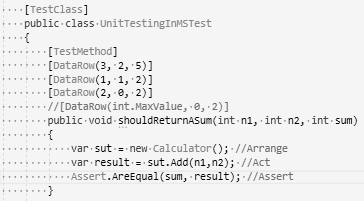
\includegraphics[width=0.5\linewidth]{Cap5/TestClass.png}
\caption{Exemplo de uma classe de teste}
\label{Fig:Fig7}
\end{figure}

\hspace{1cm}De seguida, para dar início a esta \textit{guideline}, irá ser delineada a estratégia para a execução dos testes num contexto próximo da realidade. Para tal, foi verificada, através do desenvolvimento de testes unitários, a funcionalidade da soma de dois números inteiros e foi verificado também que caso exista um número \textit{null} a soma não será executada. Este procedimento foi executado em cada \textit{framework} de testes e terá vários cenários de teste, dentro do mesmo contexto, com objetivos semelhantes.
\hspace{1cm}Tendo em conta que o desenvolvimento será orientado aos testes, será dado início através da criação de um projeto de teste. O tipo de \textit{framework} selecionada para o primeiro desenvolvimento é indiferente pelo que fica à escolha do leitor. No entanto, para estudar a viabilidade de cada uma das \textit{frameworks} de teste, foi utilizado:
\begin{itemize} 
  \item \textbf{C\#}, mais concretamente, \textbf{dotnet core} v2.2;
  \item Test Frameworks: \textbf{xUnit (2.4.0)}, \textbf{NUnit (3.11.0)} e \textbf{MSTest (1.4.0)};
\end{itemize}

\hspace{1cm}A classe que se pretende implementar apenas possui um método de adição que aceita dois inteiros caso sejam \textit{non-nullable} e retorna o valor da soma de ambos. É um método simples, cujo objetivo é somente a validação da funcionalidade de teste para permitir posterior utilização numa aplicação mais complexa.

\hspace{1cm}A solução contém o projeto \textbf{\textit{ModelClasses}} que mais tarde será o \textit{package} -- com a classe \textit{Calculator} -- juntamente com os três projetos de teste das três diferentes \textit{frameworks} (\ref{Fig:Fig8}).

\begin{figure}[hbt!]
\centering
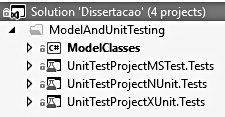
\includegraphics[width=0.35\linewidth]{Cap5/SolutionStructure.png}
\caption{Estrutura da solução}
\label{Fig:Fig8}
\end{figure}

\subsection{Tempo de execução dos testes}

\hspace{1cm}O tempo de execução das \textit{frameworks} de teste ($t_{n}$) será medido através de 9 tentativas. Este intervalo de tempo será estimado em milissegundos e será feita a média de tempo de execução para cada uma das \textit{frameworks}.

\begin{center}
 \begin{tabular}{||c | c | c | c | c | c | c | c | c | c | c ||} 
 \hline
 \textit{Framework} & \textit{$t_{1}$} & \textit{$t_{2}$} & \textit{$t_{3}$} & \textit{$t_{4}$} & \textit{$t_{5}$} & \textit{$t_{6}$} & \textit{$t_{7}$} & \textit{$t_{8}$} & \textit{$t_{9}$} & Média (ms)\\ [0.5ex] 
 \hline\hline
 MSTest & 87 & 79 & 90 & 86 & 90 & 88 & 86 & 100 & 116 & 91,33\\ 
 \hline
 NUnit & 76 & 59 & 58 & 60 & 55 & 55 & 64 & 60 & 56 & 60,33\\
 \hline
 XUnit & 62 & 50 & 42 & 54 & 44 & 43 & 53 & 46 & 48 & 49,11\\ [1ex] 
 \hline
\end{tabular}
\end{center}

\hspace{1cm}A \textit{framework} de teste com melhor performance foi o \textbf{XUnit} com um tempo médio de execução de testes de 49,11 (ms), seguido pelo \textbf{NUnit} com um tempo médio de execução de 60,33 (ms) tendo ficado o \textbf{MSTest} em último lugar, com um tempo médio de execução de 91,33 (ms). O tempo de testes foi retirado do tempo calculado pelo \textbf{IDE}, neste caso o \textit{Visual Studio 2017}, como pode ser visto na figura \ref{Fig:Fig9}.

\begin{figure}[hbt!]
\centering
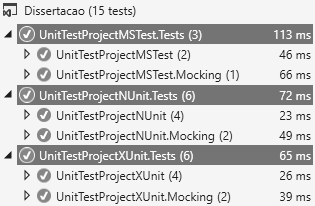
\includegraphics[width=0.5\linewidth]{Cap5/TestExplorer.png}
\caption{Explorador de testes do \textit{Visual Studio 2017}}
\label{Fig:Fig9}
\end{figure}

\subsection{Considerações}

\hspace{1cm}A empresa utiliza atualmente \textbf{MSTest} como \textit{framework} para desenvolvimento de testes. No entanto, a utilização de \textbf{XUnit} representaria uma melhoria de aproximadamente 46\% no tempo médio de execução de testes. Já a utilização de \textbf{NUnit} representaria uma melhoria de aproximadamente 34\% no tempo médio de execução de testes. Tendo em conta que o \textbf{MSTest} foi a \textit{framework} com pior performance e estando à disposição no mercado mais do que uma solução \textit{open-source} com performance evidentemente superior, o tempo de execução dos testes unitários pode ser otimizado quer com a utilização de \textbf{XUnit}, quer com a utilização de \textbf{NUnit}.

\hspace{1cm}Sendo o próximo objetivo a construção de uma \textit{pipeline} de integração e entrega contínua, que implica o desenvolvimento de testes de integração e performance, foi necessário eleger uma \textit{framework} para o seu desenvolvimento. Uma vez que se está ainda dentro da temática dos testes, ficou decidido -- juntamente com a orientação -- que seria utilizado \textbf{XUnit} daqui em diante, no desenvolvimento dos testes de integração, dada a sua rapidez de execução.

\section{Construção da \textit{pipeline} de integração contínua}

\hspace{1cm}Neste capitulo foi anteriormente desenvolvido um módulo de soma de dois números inteiros, através da utilização de \textbf{TDD}. Neste segmento, vai ser explicado todo o processo de criação de testes unitários e implementação de funcionalidades através da utilização de \textbf{XUnit} como \textit{framework} de desenvolvimento orientado a testes. De seguida, será delineado o processo de criação da \textit{pipeline}, com a comunicação com o sistema de controlo de versões (\textbf{GitLab}) em primeiro lugar, seguida pelo desenvolvimento da funcionalidade e da comunicação com \textbf{Jenkins} via \textbf{SSH}. Por último serão iniciadas duas instâncias, uma do \textbf{Nexus Repository OSS} e outra do \textbf{SonarQube} que serão o repositório de artefactos e ferramenta de análise estática respetivamente.

\subsection{Configuração do sistema de controlo de versões}

\hspace{1cm}A configuração dos repositórios varia consoante o tipo de projeto. Para este caso, em particular, é pretendido implementar-se uma \textit{pipeline} de testes automatizada com execução de testes unitários, análise estática, \textit{packaging} e \textit{push} da funcionalidade para um repositório remoto. Como vai ser necessário um repositório \textbf{.git}, onde será publicado o código da funcionalidade desenvolvida em formato não executável, faz sentido dar-se início pela comunicação entre o ambiente integrado de desenvolvimento -- onde é desenvolvida a funcionalidade -- e o repositório online que vai armazenar o código. 
\subsubsection{Criação de \textit{SSH keys}}

\hspace{1cm}Como foi explicado anteriormente, a comunicação via \textbf{SSH} exige que seja criado um \textit{key pair}. Para se criar o par de chaves, depois de estar instalado o \textbf{.git}, abre-se a linha de comandos, o \textbf{Git Bash}, e executa-se a instrução de criação de chaves  \colorbox{gray}{\textcolor{white}{\$ ssh-keygen -t rsa -b 4096 -C e-mail@exemplo.com}} que vai criar uma chave nova, utilizando o e-mail providenciado como um parâmetro de configuração que é único para cada utilizador. De seguida somos solicitados a dar um nome ao ficheiro onde se pretende guardar a chave recentemente criada e, caso se pressione \textit{Enter}, será utilizada a localização por defeito para guardar ficheiros. Com o destino seja validado, somos novamente solicitados, desta vez para criar uma password e reinserir a password. Quando o processo de criação do par de chaves é bem sucedido, é gerada uma \textit{fingerprint}, com uma imagem \textit{randomart} como mostrado na figura \ref{Fig:Fig10}. 

\hspace{1cm}Deste processo resultam dois ficheiros, um ficheiro contém a chave privada e outro contém a chave pública. A chave pública irá ser utilizada pelo \textbf{GitLab} para comunicar com a máquina onde está instalada a instância do \textbf{Jenkins} . A chave privada deve ser armazenada de forma segura \cite{gitssh}.

\begin{figure}[hbt!]
\centering
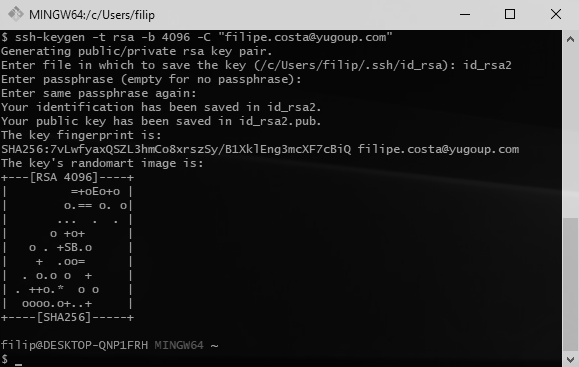
\includegraphics[width=0.6\linewidth]{Cap5/SSHKeyPairGeneration.png}
\caption{Consola de \textbf{Git Bash}}
\label{Fig:Fig10}
\end{figure}

\subsubsection{Comunicação via \textit{SSH}}

\hspace{1cm}Para ser adicionada a chave pública no \textbf{GitLab}, após serem acedidas as definições do utilizador, clica-se na opção \textit{SSH Keys} (\ref{Fig:Fig11}) e insere-se a chave pública -- o ficheiro com a terminação \textbf{.pub} -- que é um dos ficheiros gerados anteriormente. Pode optar-se também pela atribuição de um nome à chave e adição dessa chave ao conjunto de chaves. Depois de criado um par de chaves, é criado um novo repositório na interface web do \textbf{GitLab} que será clonado para a máquina.

\begin{figure}[hbt!]
\centering
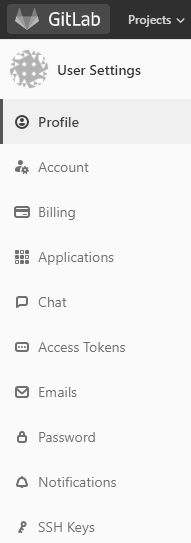
\includegraphics[width=0.2\linewidth]{Cap5/GitLabSettingsNavbar.png}
\caption{Menu de definições do utilizador do \textbf{GitLab}}
\label{Fig:Fig11}
\end{figure}

\hspace{1cm}Para clonar o repositório para a máquina é aberta a linha de comandos e executada a instrução \colorbox{gray}{\textcolor{white}{\$ git clone git@gitlab.com:nome\_utilizador/repositorio.git}}. De seguida seremos solicitados para inserir a password com a qual foi anteriormente criada a chave, ficando assim criada a pasta do projeto com ligação ao sistema de repositórios. A partir deste instante, todo o desenvolvimento da funcionalidade irá estar sincronizado entre o \textbf{GitLab} e o \textbf{Visual Studio} através do \textit{Team Explorer} que é uma ferramenta de integração de código desenvolvida e mantida pela equipa da \textbf{Microsoft} \cite{gitclone}.

\subsection{Desenvolvimento de testes unitários}

\hspace{1cm}Se o objetivo for desenvolver um \textit{package} seguindo a metodologia \textbf{TDD} o ideal será começar pela criação do projeto de teste. Como pode ser visto na figura \ref{Fig:Fig12}, terá de se alterar o nome do projeto para o nome pretendido.

\begin{figure}[hbt!]
\centering
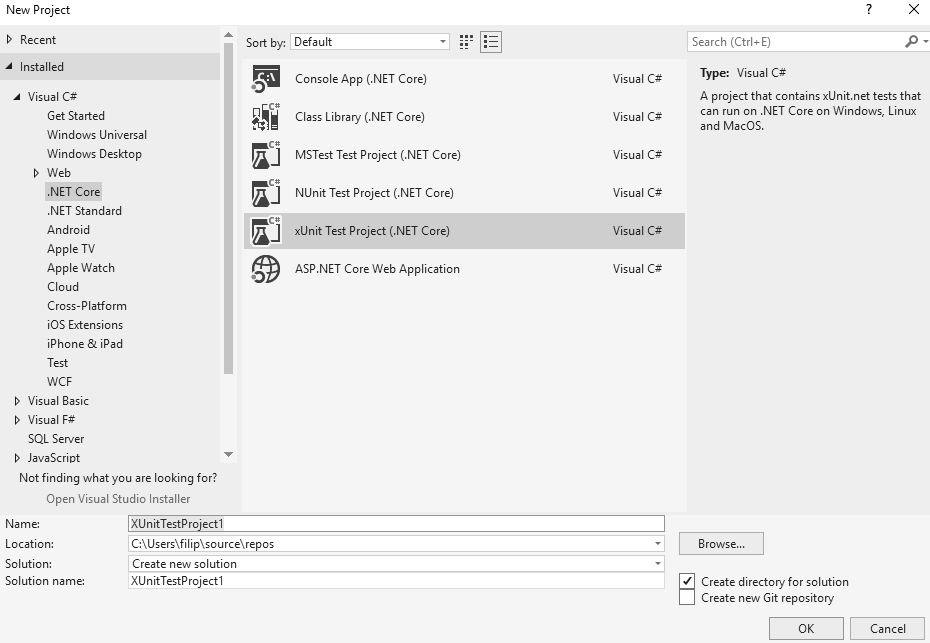
\includegraphics[width=0.7\linewidth]{Cap5/TestProjectCreation.png}
\caption{Menu de criação do projeto no \textit{Visual Studio 2017}}
\label{Fig:Fig12}
\end{figure}

\hspace{1cm}Após a criação do projeto de teste, são adicionados ao projeto os dois packages que são necessários para o desenvolvimento dos testes. São eles o \textbf{xUnit} e o \textbf{xUnit.runners.visualstudio} (\ref{Fig:Fig13}). 

\begin{figure}[hbt!]
\centering
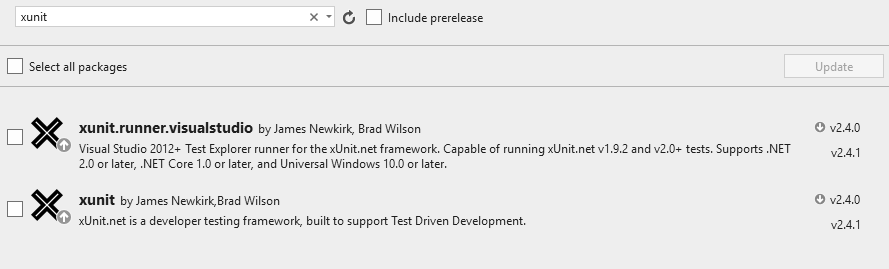
\includegraphics[width=0.7\linewidth]{Cap5/XUnitDependencies.png}
\caption{Biblioteca de \textit{packages} do \textit{Visual Studio 2017}}
\label{Fig:Fig13}
\end{figure}

\hspace{1cm}No desenvolvimento dos testes serão criados dois métodos. Um será utilizado para verificar se o resultado da soma é igual ao resultado esperado, outro para verificar se existe algum parâmetro com valor \textbf{null}.

\subsubsection{Criação da classe e estruturação dos métodos}

\hspace{1cm}Depois dos \textit{packages} estarem concluídos e -- antes de ser definida a classe como pública -- para começar o desenvolvimento da \textit{Theory}, é muito útil o apoio da documentação oficial que a \textbf{Microsoft} e a comunidade disponibilizam para se ter uma ideia mais consolidada sobre os métodos de desenvolvimento (\textbf{AAA}) de código para testes \cite{unittestingfundamentals}.
 
\subsubsection{\textit{Theory}}

\hspace{1cm}No contexto do desenvolvimento orientado a testes, a \textit{Theory} é, à semelhança dos atributos que vemos nos métodos de uma classe \textbf{controller}, um atributo que vai definir que tipo de testes serão desenvolvidos. Uma \textit{Theory} pode ser aplicada quando são desenvolvidos múltiplos casos de teste para o mesmo método. Se o objetivo for desenvolver apenas um caso de teste para um determinado método, deve ser utilizado o atributo \textit{Fact} \cite{unittestingxunit}.

\hspace{1cm}Adiciona-se uma classe para o desenvolvimento dos testes, \textit{UnitTestingInXUnit}, muda-se o nível de acesso para \textbf{public} e é iniciado o desenvolvimento da \textit{Theory} (\ref{Fig:Fig14}).

\begin{figure}[hbt!]
\centering
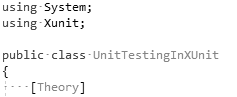
\includegraphics[width=0.4\linewidth]{Cap5/XUnitClass.png}
\caption{Classe \textit{UnitTestingInXUnit}}
\label{Fig:Fig14}
\end{figure}


\hspace{1cm}De seguida dá-se um nome, por exemplo \textit{shouldReturnASum}, ao método que é criado dentro da \textit{Theory} e passam-se três argumentos inteiros, \textbf{n1}, \textbf{n2} e \textbf{sum} (\ref{Fig:Fig15}).

\begin{figure}[hbt!]
\centering
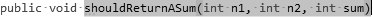
\includegraphics[width=0.6\linewidth]{Cap5/TheoryMethod.png}
\caption{Método \textit{shouldReturnASum}}
\label{Fig:Fig15}
\end{figure}


\hspace{1cm}Dentro do método, é definida uma variável -- \textbf{sut} (\textit{system under test}) -- que é onde o sistema a ser testado estará contido. Uma vez que o objetivo é criar um método para calcular a soma de dois números, o sistema a ser testado -- \textbf{sut} -- será o objeto \textit{Calculator}.

\hspace{1cm}Esta será a fase de \textit{Arrange}. O \textbf{Visual Studio}, com a ajuda do \textit{intellisense}, permite-nos criar uma classe, num ficheiro novo, com o nome do objeto, a classe \textit{Calculator} e o método \textit{Add} (\ref{Fig:Fig16}).

\begin{figure}[hbt!]
\centering
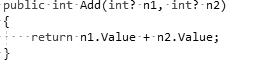
\includegraphics[width=0.4\linewidth]{Cap5/CalculatorClassAddMethod.png}
\caption{Método \textit{Add}}
\label{Fig:Fig16}
\end{figure}

\hspace{1cm}Após a criação da classe num ficheiro à parte, de volta ao projeto de teste, é iniciada a implementação da fase de \textit{Act}. Para esta fase é necessário definir outra variável chamada resultado que vai receber o resultado da soma dos dois números adicionados no método de adição. 

\hspace{1cm}Na implementação do teste, é invocado o método \textit{Add} na classe \textit{Calculator} para, só depois, se prosseguir para a fase de \textit{Assert} onde é verificado que o resultado obtido é igual ao esperado. A classe de teste deve ter sempre uma estrutura simples e organizada, com métodos à semelhança daquilo que pode ser visto na figura \ref{Fig:Fig17}. 

\begin{figure}[hbt!]
\centering
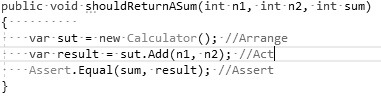
\includegraphics[width=0.5\linewidth]{Cap5/XUnitClassStructure.png}
\caption{Estrutura exemplo de um método}
\label{Fig:Fig17}
\end{figure}

\subsubsection{\textit{InlineData}}

\hspace{1cm}Para que a \textit{Theory} possa funcionar de forma correta, adiciona-se \textit{InlineData}. Estes atributos são colocados logo a seguir ao atributo \textit{Theory}. Começa-se pela adição de um caso de teste cujo resultado seja falso (e.g. 1 + 1 = 1) e outro caso de teste verdadeiro (e.g. 1 + 1 = 2) para ser feito um despiste e assim verificar-se que o método está a funcionar de acordo com o esperado (\ref{Fig:Fig18}).
 
 \begin{figure}[hbt!]
\centering
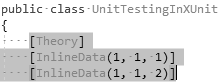
\includegraphics[width=0.3\linewidth]{Cap5/XUnitInlineData.png}
\caption{Atributos \textbf{[InlineData()]}}
\label{Fig:Fig18}
\end{figure}


\hspace{1cm}Como pode ser visto dentro do \textit{test explorer} (\ref{Fig:Fig19})
do ambiente integrado de desenvolvimento, um dos testes do método \textit{shouldReturnASum} passou e o outro teste falhou conforme esperado.

 \begin{figure}[hbt!]
\centering
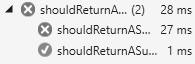
\includegraphics[width=0.3\linewidth]{Cap5/XUnitTestResults1.png}
\caption{Resultado da execução dos testes}
\label{Fig:Fig19}
\end{figure}

\hspace{1cm}Independentemente do número (\textbf{\textit{n}}) de testes que são executados, caso pelo menos um dos testes tenha resultado numa falha -- isto é caso a \textit{assertion} não se verifique -- a execução daquele método de teste (neste caso da \textit{Theory}) vai falhar completamente.

\hspace{1cm}A estrutura final da \textit{Theory}, para o caso de teste onde são adicionados dois números é relativamente simples. No entanto à medida que, para o mesmo caso, se aumenta o número cenários de teste em termos de \textit{InlineData}, aumenta também o nível de complexidade da \textit{Theory}. A \textit{Theory}, para todo o caso, ficará estruturada à semelhança daquilo que se pode ver na figura \ref{Fig:Fig20}.

 \begin{figure}[hbt!]
\centering
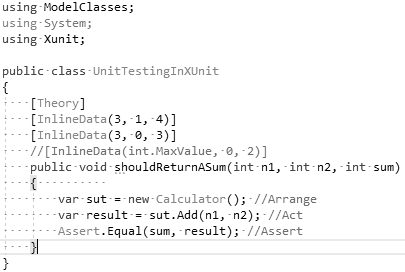
\includegraphics[width=0.5\linewidth]{Cap5/XUnitTestClassStructure2.png}
\caption{Estrutura completa de uma \textit{Theory}}
\label{Fig:Fig20}
\end{figure}

\subsubsection{Passagem de argumentos nulos}
\hspace{1cm}Pensemos no caso em que o utilizador passe um valor \textit{null} e espere que o método de adição faça \textit{output} a um resultado válido. Esta é uma validação que deve ser feita para dar seguimento à construção dos testes. Através da criação de um método de teste -- \textit{ShouldNotAddNULL} -- que simula este cenário, terá de se verificar que, caso exista um argumento \textit{null}, esse mesmo argumento será apanhado por uma exceção do tipo \textit{ArgumentNullException}.


\hspace{1cm}Para se validar que a classe \textbf{Calculator} lança uma exceção do tipo \textit{ArgumentNullException} quando algum dos dois parâmetros é nulo, é necessário em primeiro lugar adaptar a \textit{Theory} do método \textit{ShouldNotAddNULL} para que aceite valores inteiros que possam ou não existir. Para tal serão passados dois parâmetros do tipo ``\textit{int?}''. A seguir é iniciada uma instância do objeto \textbf{Calculator} -- que será o \textbf{sut} -- na fase de \textit{Arrange} para depois, nas fases de \textit{Act} e \textit{Assert} ser possível verificar que a excepção é lançada. Neste caso em particular, visível na figura \ref{Fig:Fig21}, foram agrupadas as fases de \textit{Act} e \textit{Assert} numa função \textbf{lambda}.

\begin{figure}[hbt!]
\centering
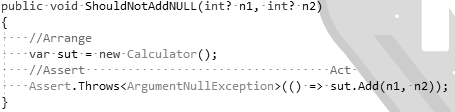
\includegraphics[width=0.6\linewidth]{Cap5/XUnitClass2.png}
\caption{Estrutura da segunda \textit{Theory}}
\label{Fig:Fig21}
\end{figure}

\hspace{1cm}Em segundo lugar, para se poderem passar números inteiros \textit{nullable}, terá de ser feita uma pequena alteração à classe \textbf{Calculator}. Em termos de estrutura, ficaria implementada -- dentro do método de adição -- uma condição (\textit{if}) que verificaria se os argumentos não são nulos. Caso exista algum argumento sem valor, é feito um \textit{throw} à exceção do tipo \textit{ArgumentNullException}. Caso contrário é retornado o resultado da soma dos dois valores (\ref{Fig:Fig22}). 

\begin{figure}[hbt!]
\centering
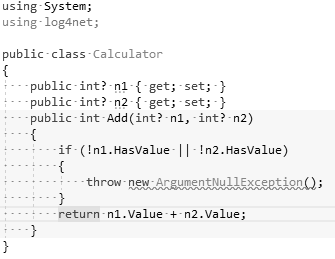
\includegraphics[width=0.5\linewidth]{Cap5/CalculatorNullArguments.png}
\caption{Estrutura da classe \textbf{Calculator} após alterações}
\label{Fig:Fig22}
\end{figure}

\hspace{1cm}De seguida, para validar que a \textit{Theory} executa os dois cenários de teste, são atribuidas duas linhas de \textit{InlineData()}. Por outras palavras, são criados dois casos de teste. O primeiro, que vai passar um valor nulo no lugar do primeiro argumento e o segundo que irá passar um valor nulo no lugar do segundo argumento. No final da adição destes casos de teste a \textit{Theory} terá aspeto semelhante ao da figura \ref{Fig:Fig23}.

\begin{figure}[hbt!]
\centering
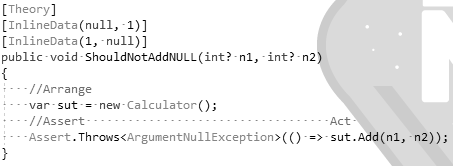
\includegraphics[width=0.5\linewidth]{Cap5/XUnitClass2Structure.png}
\caption{Estrutura da \textit{Theory} \textit{ShouldNotAddNULL} com os dois casos de teste}
\label{Fig:Fig23}
\end{figure}

\hspace{1cm}Nesta fase ambas as \textit{Theorys} estão devidamente desenvolvidas, com vários \textit{test cases}, com verificação e validação de funcionalidade. Por último lugar, para fechar a questão do desenvolvimento dos testes, são executados todos os testes para se verificar que passam como esperado (\ref{Fig:Fig24}). O código está pronto a ser publicado no sistema de repositórios.

\begin{figure}[hbt!]
\centering
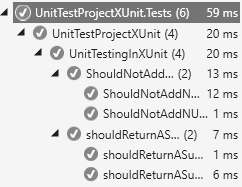
\includegraphics[width=0.4\linewidth]{Cap5/TestExplorerUnitTestingValidation.png}
\caption{Mostrador do \textit{Test Explorer}}
\label{Fig:Fig24}
\end{figure}

\subsection{Publicação do código no sistema de controlo de versões}

\hspace{1cm}No \textit{Team Explorer} podem ser publicadas as alterações feitas ao projeto, caso existam, clicando nas \textbf{Changes} (\ref{Fig:Fig25}). Depois terá de ser inserida uma mensagem que será publicada juntamente com o \textit{commit}. Nesta mensagem, é política da empresa colocar um \textit{briefing} dos ficheiros alterados, ou adicionados e, opcionalmente, pode ser especificada a funcionalidade adicionada. 

\begin{figure}[hbt!]
\centering
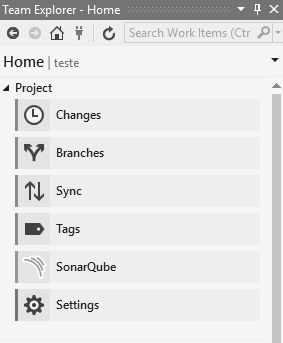
\includegraphics[width=0.4\linewidth]{Cap5/TeamExplorer.png}
\caption{Mostrador do \textit{Team Explorer}}
\label{Fig:Fig25}
\end{figure}

Clica-se em \textbf{Commit} e insere-se a password (\ref{Fig:Fig26}), gerada no momento da criação das chaves \textbf{SSH}, para que o código do projeto seja publicado no \textbf{VCS}.

\begin{figure}[hbt!]
\centering
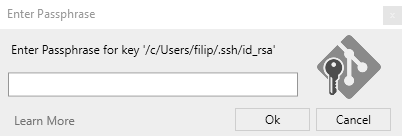
\includegraphics[width=0.5\linewidth]{Cap5/TeamExplorerSSHPassword.png}
\caption{Solicitador do \textbf{SSH}}
\label{Fig:Fig26}
\end{figure}

\hspace{1cm}Para a publicação do código deve ser utilizado um ficheiro que inclui ou exclui outro conjunto de ficheiros do projeto. Nem todos os ficheiros gerados são necessários para que o código possa ser executado. Alguns desses ficheiros são gerados automaticamente e não têm utilidade em termos de compilação. Portanto a inclusão ou exclusão deste conjunto de ficheiros -- através da utilização do \textbf{.gitignore} -- é indispensável para que numa fase mais avançada o código esteja compilável e seja reutilizável (https://github.com/github/gitignore). 

\subsection{Orquestração com \textit{Jenkins}}

\hspace{1cm}A configuração do \textbf{Jenkins} será feita na máquina de \textit{staging} disponibilizada pela empresa. A máquina está disposta em rede local. Isto torna o contacto com os dispositivos de visualização do estado das \textit{builds} mais facilitado. Mais à frente este tema é devidamente abordado.

\subsubsection{Instalação dos plugins}

\hspace{1cm}Para que possam ser executadas as \textit{builds} da compilação de código do módulo de soma, juntamente com os respetivos testes unitários e a análise estática, é necessária a instalação de um conjunto de \textit{Plugins} no \textbf{Jenkins}, nomeadamente:

\begin{itemize}
 \item Credentials;
 \item MSBuild Plugin;
 \item Gitlab Plugin;
 \item Blue Ocean (opcional);
 \item Slack Notification (opcional);
\end{itemize}

Da lista acima é obrigatório o uso dos \textit{plugins} \textbf{Credentials}, \textbf{MSBuild} e \textbf{Gitlab}, utilizados para compilação de código do projeto C\#. O \textbf{Credentials} faz a gestão das credenciais de acesso ao repositório do sistema de controlo de versões sem que estas sejam expostas. O \textbf{MSBuild} é a plataforma utilizada para fazer \textit{build} de projetos \textbf{.NET}. O \textbf{Gitlab} é utilizado para estabelecer uma ligação segura ao \textbf{VCS}. Os restantes \textit{plugins} são opcionais dado que o \textbf{Blue Ocean} é uma interface de visualização do \textbf{Jenkins} que apenas apresenta uma interface gráfica mais apelativa para o utilizador. Já o \textbf{Slack Notification} é um componente adicional para o sistema de visualização, caso se pretenda que os \textit{developers} recebam notificações no \textit{Slack} -- canal de comunicação utilizado pela empresa -- sobre os diferentes acontecimentos durante as fases da \textit{pipeline}.

\subsubsection{Instalação dos módulos de desenvolvimento do C\#}

\hspace{1cm}Será necessário descarregar o \textbf{.NET Core SDK}, que já inclui o \textbf{.NET Core Runtime}, tendo sempre em mente o sistema operativo que é utilizado. Neste caso é utilizado o \textbf{Windows 10}. Estes componentes podem ser descarregados a partir do site oficial da \textbf{Microsoft}.

Com o \textit{Software Development Kit} (SDK) devidamente instalado, neste caso na máquina de \textit{staging}, procede-se à configuração do \textbf{Jenkins}. Como dito anteriormente, esta ferramenta de integração contínua fará \textit{fetch} ao código presente no sistema de controlo de versões via \textbf{SSH} para depois poderem ser feitas operações sobre o mesmo. Para que tal seja possível, providencia-se ao orquestrador de processos a chave pública para que possa comunicar com o \textbf{GitLab} e é indicado, nas opções de configuração do \textbf{Jenkins}, o caminho da localização do \textbf{MSBuild} instalado anteriormente na máquina.

\subsubsection{Configuração das credenciais de acesso ao GitLab}

\hspace{1cm}Com o \textit{plugin} de gestão de credenciais (\textbf{Credentials}) instalado, é adicionada uma nova credencial de acesso. Para tal, clica-se em cima do \textit{plugin} \textbf{Credentials} e acede-se à opção que foi expandida, ``System'' (\ref{Fig:Fig28}).

\begin{figure}[hbt!]
\centering
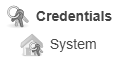
\includegraphics[width=0.15\linewidth]{Cap5/JenkinsCredentials.png}
\caption{\textit{Plugin} \textbf{Credentials}}
\label{Fig:Fig28}
\end{figure}

\hspace{1cm}De seguida clica-se em \textit{Global credentials} e adiciona-se uma nova credencial (\textit{Add Credentials}). Depois, seleciona-se o tipo de credencial na \textit{dropdownlist} como ``SSH Username with private key'' e insere-se diretamente a chave privada, selecionando a opção ``Enter directly'', no campo ``Private Key'', como pode ser visto na figura \ref{Fig:Fig29}.

\begin{figure}[hbt!]
\centering
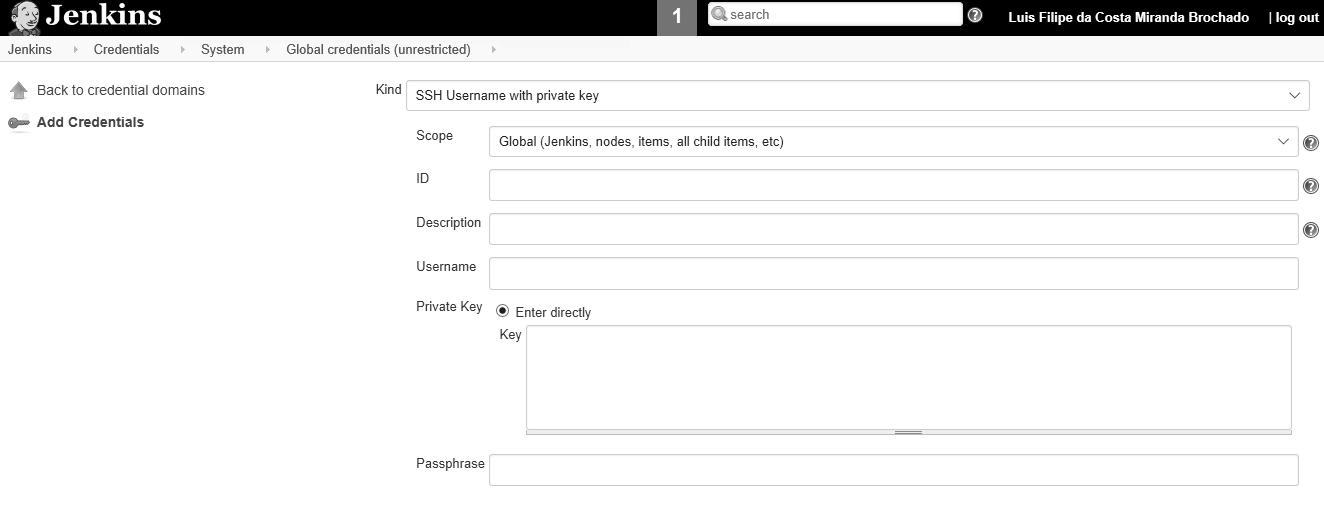
\includegraphics[width=0.9\linewidth]{Cap5/JenkinsCredentialsConfig.png}
\caption{Configuração das credenciais de acesso}
\label{Fig:Fig29}
\end{figure}

\subsubsection{Configuração do \textbf{MSBuild}}

\hspace{1cm}Nas opções de configuração do \textbf{Jenkins}, em \textbf{Manage Jenkins}, existe um conjunto de opções à disposição. Será selecionada a opção \textbf{Global Tool Configuration}. Se o \textit{plugin} \textbf{MSBuild} tiver sido instalado, deverá aparecer nas opções de instalação uma imagem semelhante à da figura \ref{Fig:Fig30}. 

\begin{figure}[hbt!]
\centering
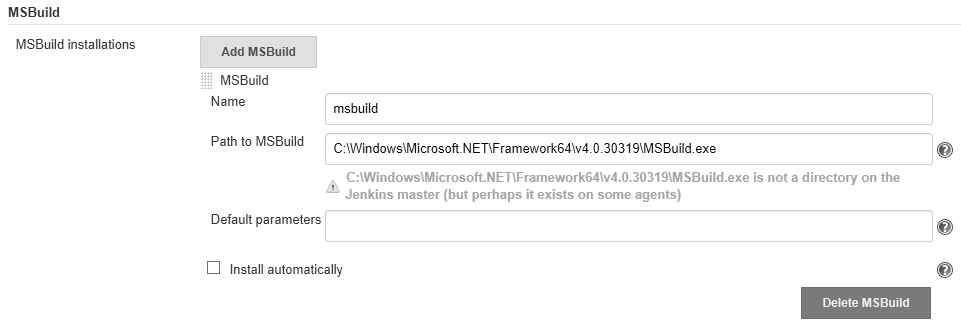
\includegraphics[width=0.9\linewidth]{Cap5/JenkinsGlobalToolConfiguration.png}
\caption{Caminho de instalação do \textbf{MSBuild}}
\label{Fig:Fig30}
\end{figure}

\hspace{1cm}Com o caminho absoluto do ficheiro executável do \textbf{MSBuild} colocado na opção ``Path to MSBuild'', o orquestrador de processos está pronto a compilar o código dos projetos \textbf{.NET}. Nesta fase a configuração do orquestrador está concluída. De seguida será abordada a configuração da \textit{pipeline} testes automatizados.

\subsection{Configuração da \textit{pipeline}}

\hspace{1cm}Começando pela criação de um \textit{New Item}, é atribuído um nome à escolha do utilizador selecionando a opção \textit{Freestyle project}. O primeiro \textit{job} está criado e segue-se sua configuração. Este \textit{job} será o primeiro componente da \textit{pipeline}.

\subsubsection{Estrutura dos \textit{jobs}}

\hspace{1cm}Para a configuração começa-se por dar uma descrição ao \textit{job} e por selecionar a opção para descartar builds anteriores -- ``Discard old build'' -- para que sejam eliminados todos os ficheiros e artefactos resultantes de compilações de código anteriores. Depois adiciona-se o \textbf{GitLab Plugin} à lista de \textit{plugins} para que seja possível configurar uma ligação ao \textbf{VCS} através da criação de um \textbf{API token}. Para configurar esta ligação é necessário aceder novamente às propriedades de configuração do sistema -- \textbf{Configure System} -- e navegar até aparecer a secção de configuração do \textbf{GitLab} (\ref{Fig:Fig31}).

\begin{figure}[hbt!]
\centering
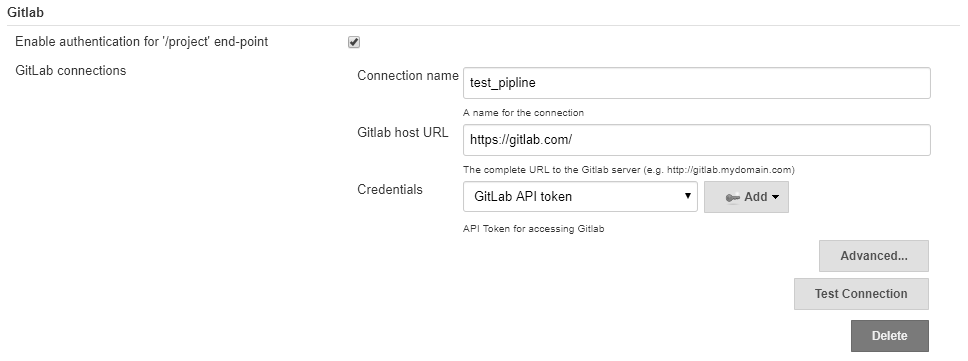
\includegraphics[width=0.9\linewidth]{Cap5/ConfigureSystem.png}
\caption{Configuração da ligação ao \textbf{GitLab}}
\label{Fig:Fig31}
\end{figure}

\hspace{1cm}Antes de ser adicionado um \textit{Access Token} ao orquestrador de processos é necessário requisitar, dentro do sistema de controlo de versões, um novo \textit{Personal Access Token}. Para tal, acede-se à plataforma \textbf{GitLab}, navega-se até aos \textit{user settings}, clica-se em \textit{Access Tokens} e adiciona-se um nome, uma data de validade e os \textbf{scopes} do \textit{token} como mostrado na figura \ref{Fig:Fig32}.

\begin{figure}[hbt!]
\centering
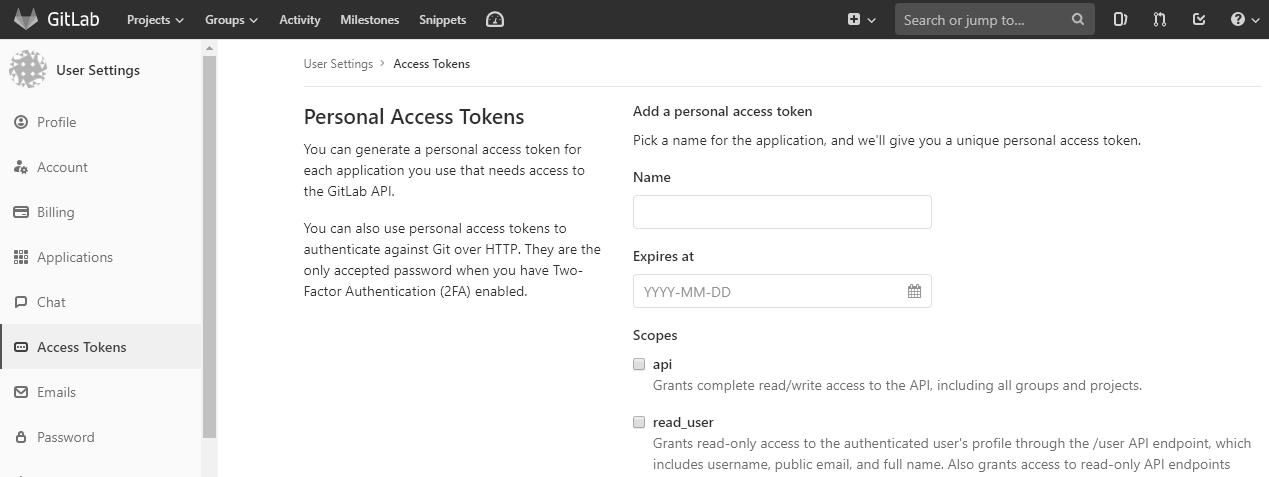
\includegraphics[width=0.9\linewidth]{Cap5/GitLabAccessToken.png}
\caption{Menu de criação do \textit{Personal Access Token} }
\label{Fig:Fig32}
\end{figure}

O \textit{access token} criado será depois adicionado nas credenciais do \textbf{Jenkins}. Este \textit{access token} só pode ser visualizado uma única vez por questões de segurança e, por boa prática, não deve ser utilizado em mais que um serviço.

\hspace{1cm}Voltando à configuração do \textit{job}, com a \textit{GitLab Connection} configurada, seguem-se as configurações de \textbf{Source Code Management}. É aqui que serão configuradas a ligações via \textbf{SSH} aos respetivos repositórios criados que foram armazenados no \textbf{VCS}. Assim sendo seleciona-se a opção \textbf{Git} e preenche-se o \textbf{URL} do repositório com a hiperligação do protocolo \textbf{SSH}, com as respetivas credenciais de acesso, que é o meio de ligação pretendido para estabelecer a conexão. A \textit{branch} que será utilizada para fazer \textit{build} é a única existente no projeto (\ref{Fig:Fig33}), \textbf{master}.

\begin{figure}[hbt!]
\centering
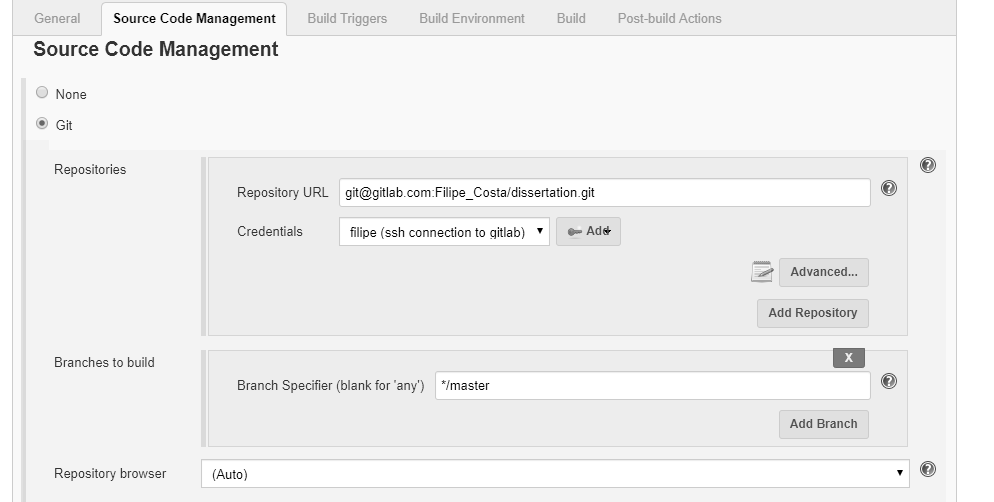
\includegraphics[width=0.9\linewidth]{Cap5/JenkinsSourceCodeManagement.png}
\caption{\textit{Source Code Management}}
\label{Fig:Fig33}
\end{figure}

\hspace{1cm}O próximo separador, \textbf{Build Triggers}, vai ser passado à frente uma vez que não é necessário qualquer tipo de configuração neste campo. Este segmento -- \textbf{Build Triggers} -- é onde são agendados \textit{triggers} automáticos a novas \textit{builds} mediante certos eventos. Será utilizado mais à frente, por exemplo, na configuração dos \textit{jobs} que serão dependentes da execução deste primeiro \textit{job}.

\hspace{1cm}No próximo segmento, \textbf{Build Environment}, é selecionada a opção ``Delete workspace before build starts''. Esta opção, segundo a tradução literal do Inglês, significa que é apagado o \textit{worskpace} gerado pelo \textbf{Jenkins} sempre que começar uma \textit{build} (\ref{Fig:Fig34}). 

\begin{figure}[hbt!]
\centering
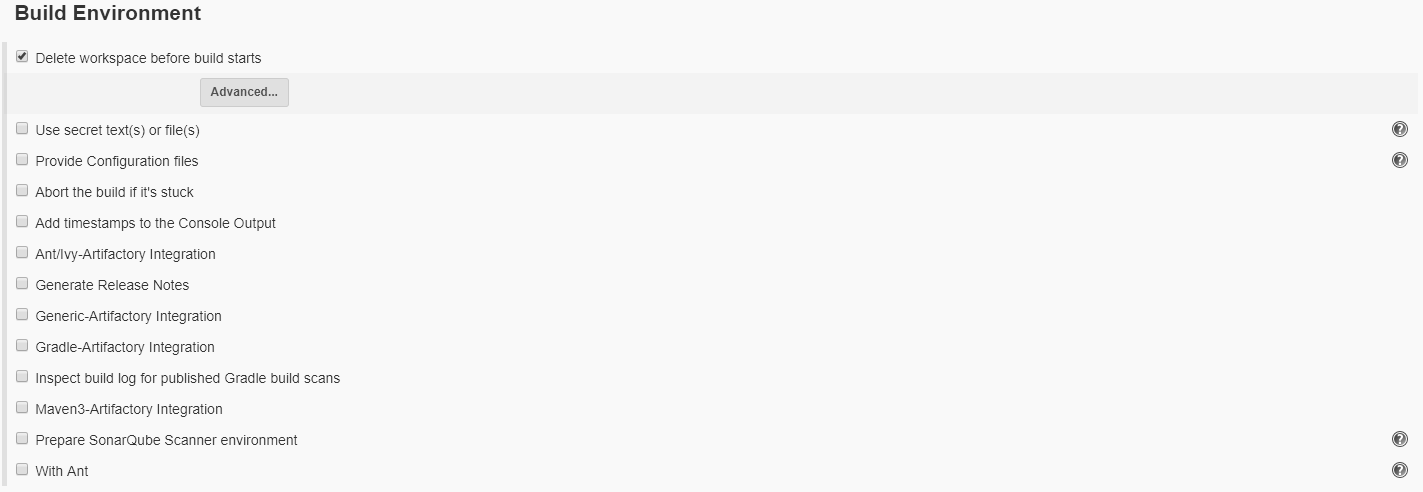
\includegraphics[width=0.9\linewidth]{Cap5/JenkinsBuildEnvironment.png}
\caption{\textit{Build Environment}}
\label{Fig:Fig34}
\end{figure}

Esta funcionalidade tem como objetivo evitar que execuções anteriores da \textit{pipeline} provoquem erros devido a versões de serviços e/ou dependências antigas que tenham sido usados e não tenham sido atualizados corretamente para a nova execução.

\subsection{Integração dos serviços}

\hspace{1cm}Para a integração de serviços externos na \textit{pipeline} vão ser utilizados:

\begin{itemize}
 \item \textbf{Docker};
 \item \textbf{SonarQube};
 \item \textbf{Nexus Repository Manager OSS 2};
 \item \textbf{Docker Registry 2.0};
\end{itemize}

\hspace{1cm}Na fase de \textit{\textbf{Build}}, vão ser inseridas as instruções que normalmente seriam introduzidas numa linha de comandos. Para que estejamos mais contextualizados com as instruções que são utilizadas aconselha-se a consulta da documentação oficial de apoio da \textbf{Microsoft} referente ao \textbf{.NET Core CLI} \cite{dotnetcorecli}. Toda a informação que é necessária está disponível nesta documentação.

\subsubsection{Integração com \textbf{SonarQube}}

\hspace{1cm}Comecemos por integrar a análise estática na \textit{pipeline}. Para fazer a análise estática do código é utilizada uma \textit{tool} de revisão de código chamada \textbf{SonarQube}. Esta ferramenta de análise estática já integra com \textbf{Docker} portanto vai ser executada uma instância de uma versão do \textbf{SonarQube} dentro de um \textit{container} que será publicado na porta 9000. Todos os dados serão guardados dentro de um \textit{container} do \textbf{Docker} que foi anteriormente criado através de uma técnica de persistência de dados em volume \cite{dockervolumes}. Desta forma, sempre que for necessário, os dados podem ser acedidos através do \textit{attachment} de um \textit{container} a este volume de dados conferindo assim a possibilidade e a garantia de se utilizar uma instância para aceder às informações guardados sobre os projetos. 

\hspace{1cm}A configuração de um projeto dentro da instância do \textbf{SonarQube} é relativamente simples. As credenciais de autenticação, por defeito, são \colorbox{gray}{\textcolor{white}{admin}} para o \textbf{username} e \colorbox{gray}{\textcolor{white}{admin}} para \textbf{password}. Todos os projetos são criados da mesma forma, independentemente da linguagem utilizada. Neste caso é selecionada a opção ``criar novo projeto'' e, após a atribuição de uma chave e de um nome ao projeto, adiciona-se um \textit{token} de identificação. De seguida é selecionada a linguagem em que o projeto foi desenvolvido. É importante ter em consideração que tanto a atribuição do \textit{token} como a seleção da linguagem em que o projeto foi desenvolvido são dois passos que também têm relevância para a integração do \textbf{SonarQube} com a \textit{pipeline}. Mais tarde será necessário a chave que atribuída ao projeto nesta fase. 

\hspace{1cm}A instrução que se vai utilizar para dar início à análise estática é a seguinte: \colorbox{gray}{\textcolor{white}{\$ dotnet SonarScanner.MSBuild.dll begin /k:``project-key''}} e caso se pretenda, por exemplo, executar a análise estática a partir de um \textit{container} dentro de uma máquina virtual, podem ser adicionadas como opções \colorbox{gray}{\textcolor{white}{/d:sonar.host.url=``hostname''}} para indicar o \textit{hostname} onde será feita análise e \colorbox{gray}{\textcolor{white}{/d:sonar.login=``access\_token''}} para indicar o \textit{access token} que permite aceder ao \textit{container}. É necessário ter em conta que o \textbf{Jenkins} não reconhece nem o comando \textit{dotnet}, nem a ``.dll'' do \textit{SonarScanner}, portanto são necessários os \textit{absolute paths} destes dois ficheiros dentro da máquina principal para que o orquestrador os consiga encontrar (\ref{Fig:Fig35}).

\begin{figure}[hbt!]
\centering
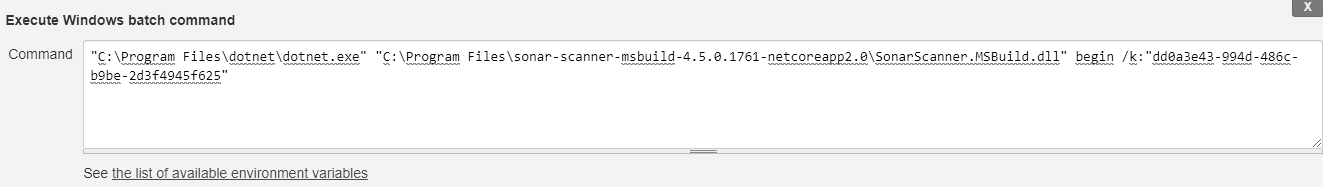
\includegraphics[width=0.9\linewidth]{Cap5/JenkinsSonarQubeStart.png}
\caption{Primeira instrução do \textbf{SonarQube}}
\label{Fig:Fig35}
\end{figure}

\hspace{1cm}Para concluir a análise estática é necessário utilizar como última instrução: \colorbox{gray}{\textcolor{white}{\$ dotnet SonarScanner.MSBuild.dll end}} (\ref{Fig:Fig36}). No caso em que a análise estática é iniciada com as opções extra, é necessário executar a instrução descrita neste parágrafo com a adição da opção \colorbox{gray}{\textcolor{white}{/d:sonar.login=``access\_token''}} para encerrar corretmente a execução da análise estática.

\begin{figure}[hbt!]
\centering
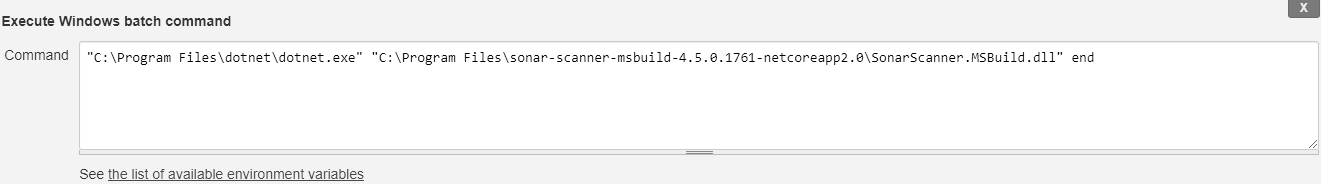
\includegraphics[width=0.9\linewidth]{Cap5/JenkinsSonarQubeFinish.png}
\caption{Última instrução do \textbf{SonarQube}}
\label{Fig:Fig36}
\end{figure}

\hspace{1cm}Executa-se a instrução para iniciar a ferramenta de análise estática no início do \textit{job} para que -- durante as fases de \textit{build} e \textit{testing} -- todo o código da aplicação seja revisto. É executada a instrução para terminar a ferramenta antes do final do \textit{job} para que seja parada a execução desta \textit{tool} \cite{sonarqubejenkins}. Os resultados da análise estática serão apresentados à semelhança daquilo que se pode ser visto na figura \ref{Fig:Fig37}.

\begin{figure}[hbt!]
\centering
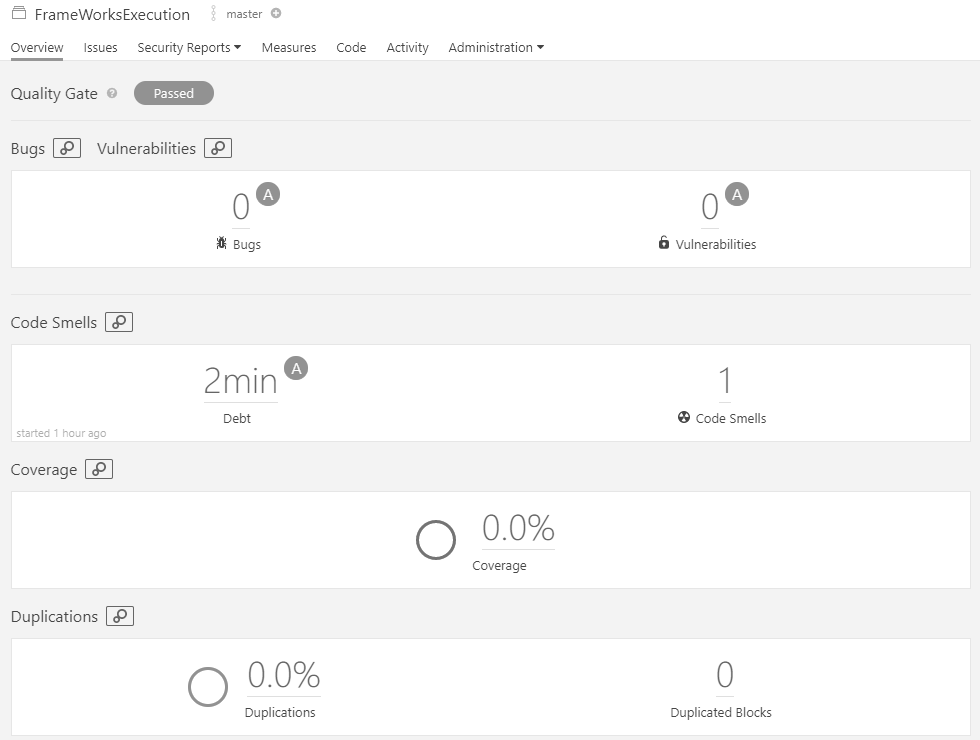
\includegraphics[width=0.8\linewidth]{Cap5/SonarQube.png}
\caption{SonarQube -- Quality Gate}
\label{Fig:Fig37}
\end{figure}

\subsubsection{\textit{Build} do projeto e dos testes}

\hspace{1cm}Para se fazer \textit{build} a um projeto (.csproj) ou a uma solução (.sln) a instrução é: \colorbox{gray}{\textcolor{white}{\$ dotnet build project-path}} \cite{dotnetbuild}. Aqui entramos na fase de \textit{build} (\ref{Fig:Fig38}) do projeto e dos testes unitários que foram criados para a aplicação calculadora.

\begin{figure}[hbt!]
\centering
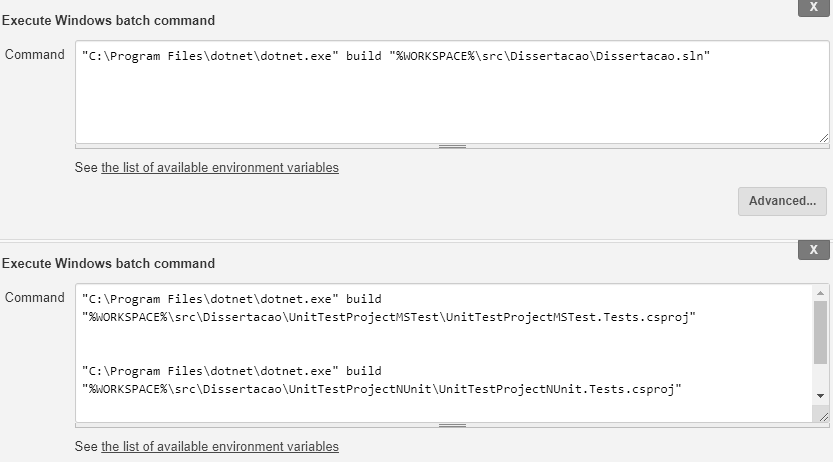
\includegraphics[width=0.9\linewidth]{Cap5/JenkinsProjectBuild.png}
\caption{Instruções de \textit{build} dos projetos}
\label{Fig:Fig38}
\end{figure}

\hspace{1cm}Após a fase de \textit{build}, são executados os testes para o \textbf{Jenkins} interpretar os seus resultados e produzir um gráfico com a estatística dos \textit{test runs}. A instrução utilizada para produzir os resultados dos testes em formato interpretável (.trx) foi a seguinte: \colorbox{gray}{\textcolor{white}{\$ dotnet test project-path -{}-no-build -{}-logger trx}} \cite{dotnettest}.\\ Esta instrução produz um ficheiro (.trx) com o resultado dos testes que é interpretado pelo orquestrador e apresentado na GUI (\ref{Fig:Fig39}). 

\begin{figure}[hbt!]
\centering
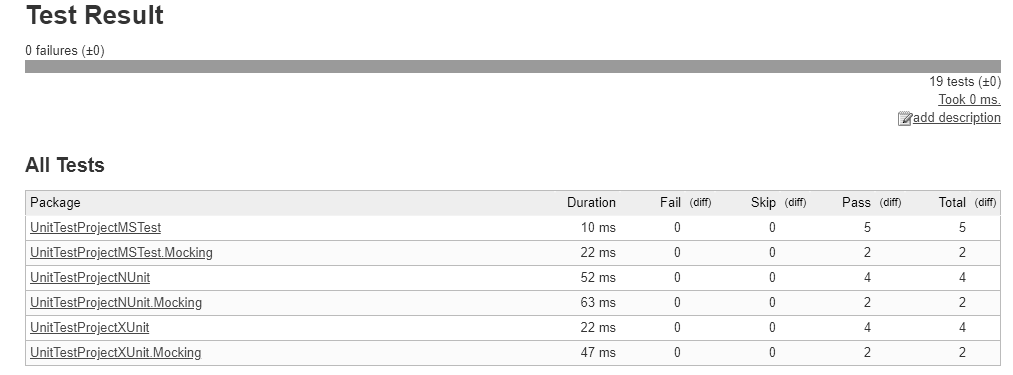
\includegraphics[width=0.9\linewidth]{Cap5/JenkinsTestResult.png}
\caption{Resultado dos testes unitários}
\label{Fig:Fig39}
\end{figure}

\subsubsection{Integração com o repositório \textit{Nexus Repository Manager OSS}}

\hspace{1cm}A ferramenta de armazenamento de artefactos utilizada é o \textbf{Nexus Repository Manager OSS}. Este sistema de gestão de artefactos tem integração com \textbf{Docker} -- que foi o motivo com mais peso na sua seleção -- e apresenta uma \textbf{GUI} de simples utilização. Para a \textit{pipeline} foi escolhida uma versão mais antiga, a versão \textbf{2.14.12-02}, uma vez que durante a escrita do documento cumpria com os requisitos estabelecidos pela orientação. A versão \textbf{2.14.13-01} também pode ser utilizada uma vez que não existem diferenças tanto em termos de utilização como de configuração.

\hspace{1cm}Para que seja possível publicar artefactos dentro de um \textit{container} com uma instância do \textbf{Nexus} é necessário realizar um conjunto de operações. Por outras palavras, é preciso empacotar o módulo de soma, \textit{ModelClasses}, para um formato específico e assim transformar o módulo de soma de dois números inteiros num \textbf{NuGet Package}. Esta operação pode ser feita através da utilização da instrução: \colorbox{gray}{\textcolor{white}{\$ dotnet pack project-path}} \cite{dotnetpack}. Esta instrução gera um ficheiro do tipo ``\textbf{.nupkg}'' que é o módulo \textit{plug-and-play} da funcionalidade desenvolvida.

\hspace{1cm}O próximo passo é a configuração do repositório. Para configurar corretamente o repositório aconselha-se a leitura da documentação produzida pela \textbf{Sonatype} \textbf{\cite{sonatypenexus}} e disponibilizada no repositório público de imagens do \textbf{Docker} \textbf{\cite{sonatypenexusdocker}}. A configuração do repositório \textbf{NuGet} requer a criação de dois repositórios, um \textit{proxy} e um \textit{hosted}, que mais tarde vão ser colocados dentro de um grupo, \textit{public}, resultando no total de três repositórios criados. As credenciais de autenticação por defeito são \colorbox{gray}{\textcolor{white}{admin}} para o \textbf{username} e \colorbox{gray}{\textcolor{white}{admin123}} para \textbf{password}. A criação dos repositórios do \textbf{Nexus} é ligeiramente mais complexa em termos processuais e, comparativamente com a configuração do \textbf{SonarQube}, requer alguns cuidados. Por defeito, o \textbf{Nexus} traz consigo um conjunto de repositórios \textbf{Maven} pré-configurados que podem ser eliminados. 

\hspace{1cm}Começando pela adição de um repositório \textit{proxy}, é atribuido o ID ``nuget-gallery-proxy'' e o nome ``Nuget Gallery Proxy''. Como pode ser visto na figura \ref{Fig:Fig40}, no campo \textit{Provider} seleciona-se \textbf{NuGet} como formato do artefacto e coloca-se a conexão à \textbf{API} pública do \textbf{NuGet} no campo \textit{Remote Storage Location}.

\begin{figure}[hbt!]
\centering
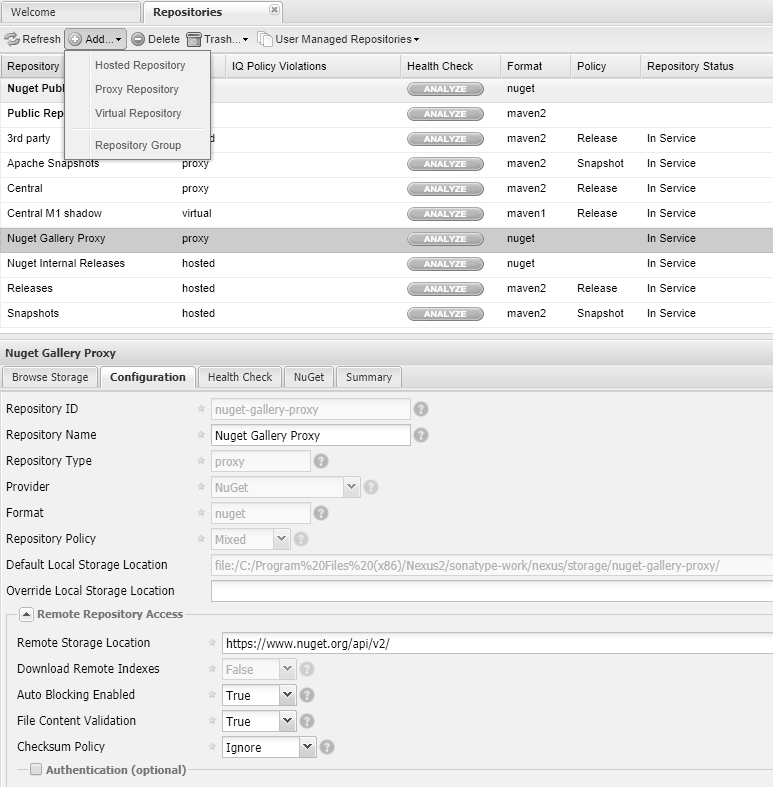
\includegraphics[width=0.9\linewidth]{Cap5/NexusOSSProxy.png}
\caption{Configuração do repositório NuGet proxy}
\label{Fig:Fig40}
\end{figure}

\hspace{1cm}De seguida cria-se o repositório \textit{hosted}, atribuindo como ID ``nuget-releases'' e como nome ``Nuget Internal Releases''. À semelhança da configuração anterior, o \textit{Provider} é o mesmo, ou seja, \textit{NuGet}. Nas definições de acesso podem ser selecionadas as opções \textit{Allow Redeploy} ou \textit{Disable Redeploy} consoante se pretenda ou não permitir \textit{overwriting} a pacotes de versões semelhantes. Para testar o repositório aconselha-se a \textit{Policy} de \textit{Allow Redeploy} uma vez que não bloqueia a entrada a \textbf{NuGet packages} da mesma versão sendo mais fácil de verificar o seu funcionamento.

\hspace{1cm}Por último, o grupo que vai conter os dois repositórios. Para configurar o grupo de repositórios no \textbf{Nexus} são apenas necessários um ID, por exemplo ``nuget-public'', e um nome semelhante, ``Nuget Public''. De seguida, passam-se os repositórios \textit{hosted} e \textit{proxy} -- presentes nos \textit{Available Repositories} -- para os \textit{Ordered Group Repositories} (\ref{Fig:Fig41}). 

\begin{figure}[hbt!]
\centering
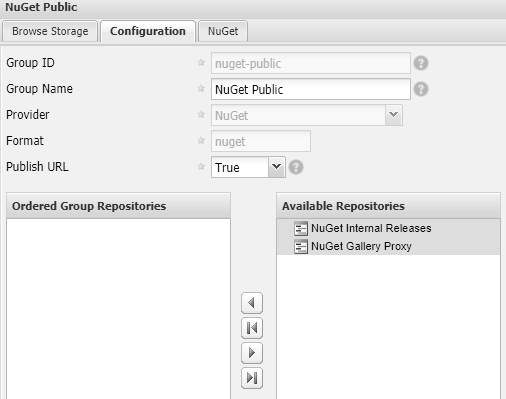
\includegraphics[width=0.9\linewidth]{Cap5/NexusPublic.png}
\caption{Configuração do repositório NuGet Public}
\label{Fig:Fig41}
\end{figure}

\hspace{1cm}A configuração do repositório de \textbf{NuGet packages} está praticamente concluída. Para publicar \textbf{Packages} no repositório é necessário aceder à API Key gerada pelo \textbf{Nexus}. Para tal, vai-se ao painel de administração na opção \textit{server} e, nas \textit{security settings}, coloca-se a \textit{NuGet API-Key Realm} nos \textbf{Selected Realms} (\ref{Fig:Fig42}).

\begin{figure}[hbt!]
\centering
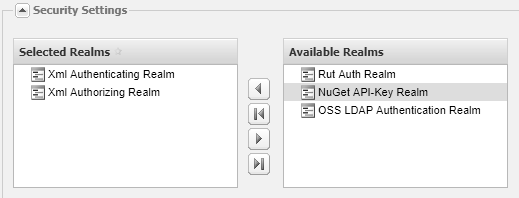
\includegraphics[width=0.9\linewidth]{Cap5/NexusSecurity.png}
\caption{Configurações de segurança do servidor Nexus}
\label{Fig:Fig42}
\end{figure}

\hspace{1cm}A \textbf{Sonatype} disponibiliza no seu canal oficial de \textbf{Youtube} um vídeo mais detalhado sobre a gestão de componentes .NET com o \textbf{Nexus} \cite{managingdotnetcomponentswithnexus}. A última instrução da fase de \textit{build} vai colocar o \textit{package} no repositório que foi configurado. Esta instrução necessita da \textbf{API Key} para autenticar contra o repositório do \textbf{Nexus}, precisa também da hiperligação (\textit{source}) para onde será enviado o pacote e precisa do caminho absoluto do ficheiro produzido com a instrução anterior. Pode utilizar-se uma instrução semelhante à seguinte:  \colorbox{gray}{\textcolor{white}{dotnet nuget push}}, com o caminho do \textit{package} \colorbox{gray}{\textcolor{white}{package-path}}, com a \textbf{API Key} \colorbox{gray}{\textcolor{white}{-k nexus-api-key}} e com a \textit{source} \colorbox{gray}{\textcolor{white}{-s hosted-repository}} como opções \cite{dotnetnuget}.

\begin{figure}[hbt!]
\centering
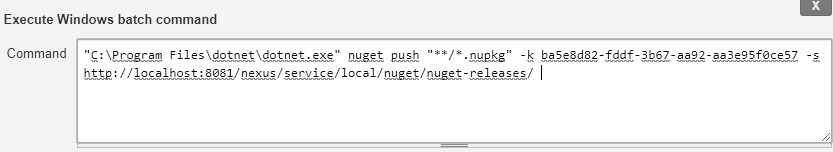
\includegraphics[width=0.9\linewidth]{Cap5/JenkinsPushToNexus.png}
\caption{Instrução de publicação do \textit{package} para o Nexus}
\label{Fig:Fig43}
\end{figure}

\hspace{1cm}A instrução é semelhante aquela visível na figura \ref{Fig:Fig43} sendo que se pode recorrer a \textit{wildcards} (*) para procurar ficheiros pelo seu formato. Está tudo configurado para se fazer \textit{build} do primeiro \textit{job} da \textit{pipeline}. O próximo passo é o desenvolvimento de uma \textbf{Web API} que implemente a funcionalidade de soma.

\subsection{Desenvolvimento da Web API}

\hspace{1cm}Para o desenvolvimento da \textbf{Web API} será utilizada uma ferramenta de documentação, o \textbf{Swagger} \cite{aboutswagger}. Esta ferramenta \textit{open source} é utilizada pela comunidade de \textit{developers} principalmente no desenvolvimento de \textbf{APIs REST}.

\hspace{1cm}Como dito anteriormente, será utilizado o \textbf{NuGet package} -- \textit{ModelClasses} -- e são também necessárias algumas alterações ao código, nomeadamente a adição do serviço de documentação do \textbf{Swagger} na classe \textit{Startup.cs}. O serviço que se vai desenvolver não incorpora uma base de dados uma vez que para testar os serviços em funcionamento não seria necessário armazenar dados da \textbf{Web API} nesta fase de desenvolvimento. 

\hspace{1cm}Depois do desenvolvimento da API, ainda dentro da mesma solução, será criado um projeto de teste onde vão ser desenvolvidos os testes de integração e performance aos \textit{endpoints} disponíveis.

\subsubsection{Pré-requisitos:}

\begin{itemize}
 \item Swashbuckle.AspNetCore (4.0.1);
 \item Swashbuckle.AspNetCore.Swagger (4.0.1);
 \item ModelClasses (1.0.3.4);
 \item Microsoft.AspNetCore.App;
 \item Microsoft.AspNetCore.App.Design;
\end{itemize}

\subsubsection{Configuração da nova \textit{source} no \textit{Visual Studio}}

\hspace{1cm}Para ser adicionada a nova \textit{source} no \textbf{Visual Studio} é necessário aceder a \textit{``Tools''} e clicar em \textit{``options''}. Depois navega-se novamente até se encontrarem as definições de configuração do \textit{``NuGet Package Manager''} e adiciona-se a nova fonte na opção \textit{``Package Sources''} para que possam ser incluídos no projeto os pacotes com as dependências necessárias (\ref{Fig:Fig44}).

\begin{figure}[hbt!]
\centering
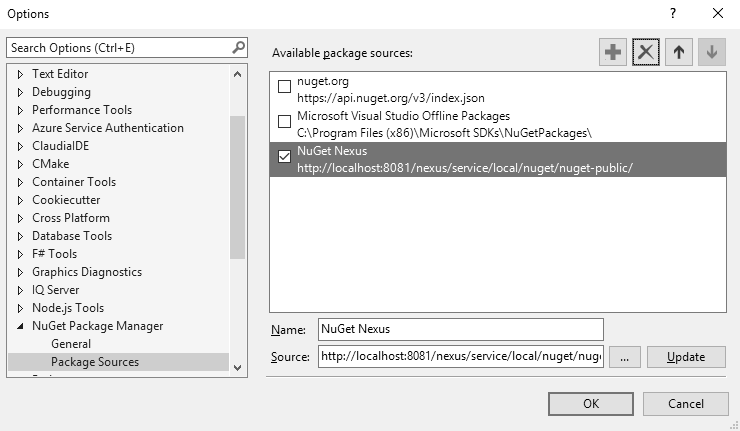
\includegraphics[width=0.7\linewidth]{Cap5/VSPackageSource.png}
\caption{NuGet Package Manager}
\label{Fig:Fig44}
\end{figure}

Todos os pacotes estão incluídos na nova \textit{source}, mesmo aqueles que são disponibilizados na API do \textbf{NuGet} (https://www.nuget.org/api/v2), porque o repositório \textit{proxy} foi configurado para incluir a API pública de \textbf{NuGet Packages}.

\subsubsection{Alterações ao serviço da Web API}

\hspace{1cm}No serviço, começa-se por editar a classe ``Startup.cs'' para incluir a interface do \textbf{Swagger}. Em primeiro lugar são incluídos os \textit{packages} do \textbf{Swashbuckle} nas dependências e, de seguida, dentro da classe incluem-se os serviços do \textbf{Swagger} nos métodos de configuração do serviço (\ref{Fig:Fig45}) e da aplicação especificada (\ref{Fig:Fig46}). A configuração do \textbf{Swagger} está, uma vez mais, em detalhe na documentação oficial \cite{dotnetwithswagger} do .NET pelo que se aconselha a sua leitura.

\begin{figure}[hbt!]
\centering
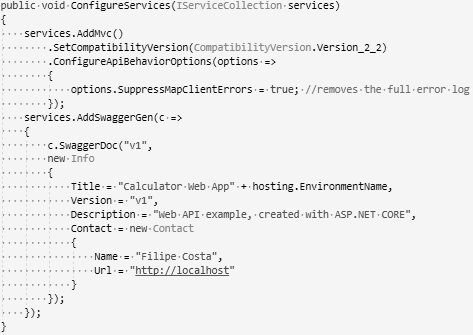
\includegraphics[width=0.65\linewidth]{Cap5/VSStartupClass1.png}
\caption{Estrutura do método de configuração do serviço}
\label{Fig:Fig45}
\end{figure}

\begin{figure}[hbt!]
\centering
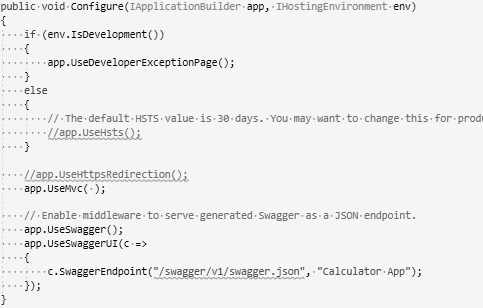
\includegraphics[width=0.65\linewidth]{Cap5/VSStartupClass2.png}
\caption{Estrutura do método de configuração da aplicação especificada}
\label{Fig:Fig46}
\end{figure}

\hspace{1cm}Na classe \textit{HomeController} está incluído por defeito um método \textit{GET} que retorna duas strings, ``value1'' e ``value2''. Este método vai permanecer tal como está sendo apenas alterado o nome do controlador para \textit{CalcController}. Com o \textbf{NuGet Package} incluído na classe, está tudo pronto para ser implementada a funcionalidade de soma na \textbf{Web API}. 

\hspace{1cm}O proximo objetivo será criar um método \textit{POST} para somar dois números inteiros. Este método, chamado \textit{PostNumbers}, vai receber dois números inteiros (\textit{int n1}, \textit{int n2}) e vai retornar o resultado da sua soma. A estrutura do método é bastante simples. É criado um novo objeto da classe \textit{Calculator}, proveniente do \textbf{NuGet Package} (\textit{ModelClasses}), depois é retornado o resultado do método \textit{Add} daquele objeto. Como se pode ver na figura \ref{Fig:Fig47}, os parâmetros que são enviados pela \textit{string}, para serem adicionados, são aqueles que serão introduzidos pelo utilizador.

\begin{figure}[hbt!]
\centering
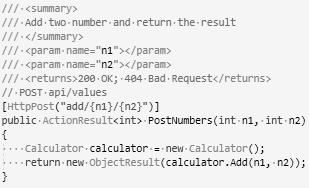
\includegraphics[width=0.45\linewidth]{Cap5/VSPostNumbers.png}
\caption{Estrutura do método \textit{PostNumbers}}
\label{Fig:Fig47}
\end{figure}

\begin{figure}[hbt!]
\centering
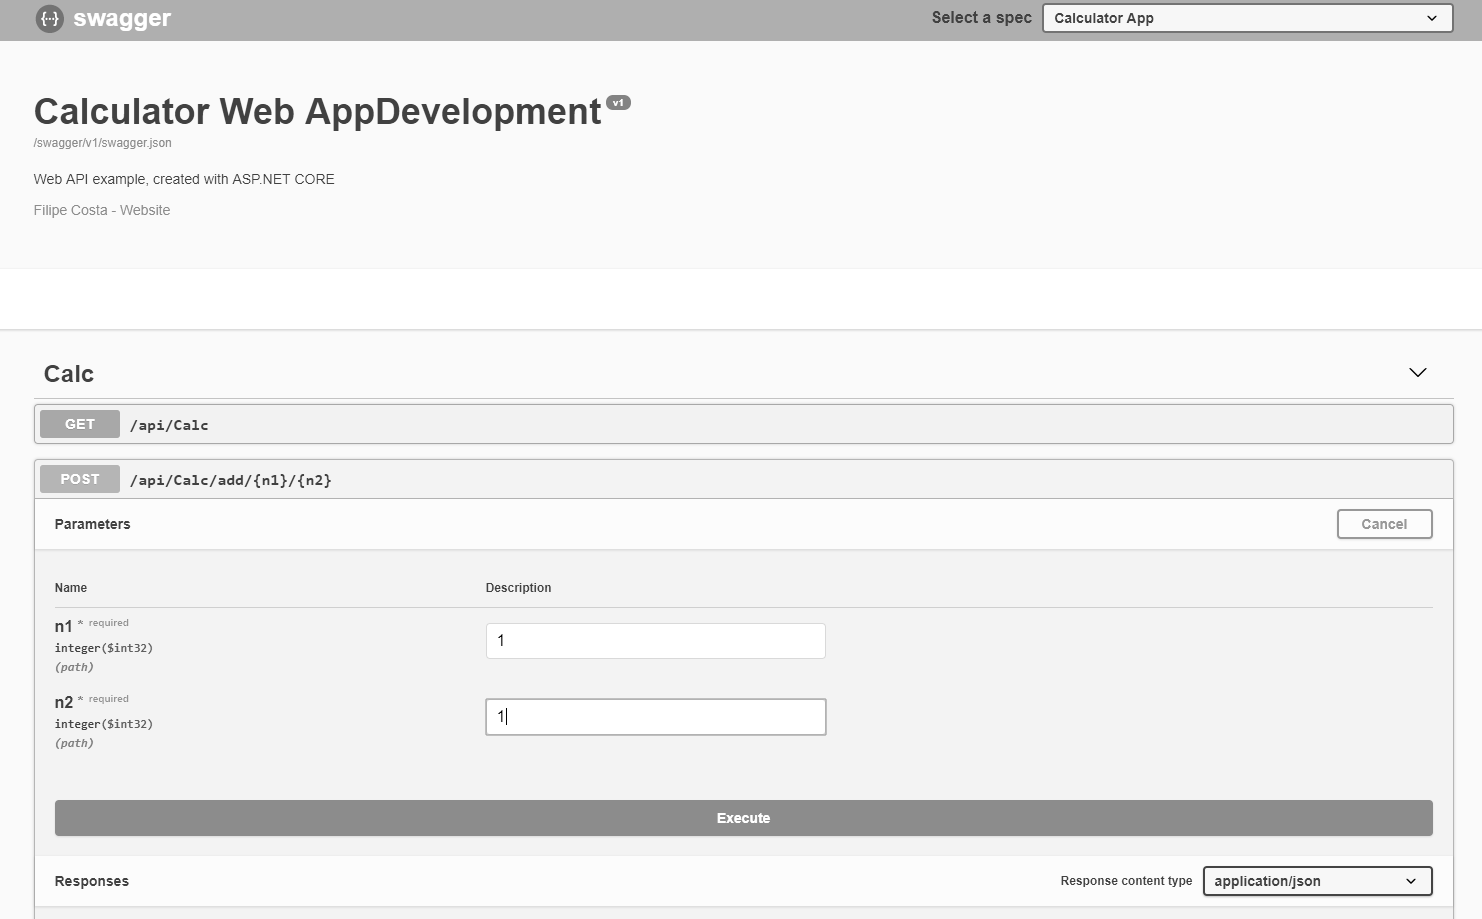
\includegraphics[width=0.8\linewidth]{Cap5/Swagger1.png}
\caption{Interface do \textbf{Swagger}}
\label{Fig:Fig48}
\end{figure}

\hspace{1cm}Para testar a \textbf{Web API} através da interface gráfica do \textbf{Swagger} deve ser executado (F5) o projeto e no \textit{browser}, após ser expandido o método \textit{POST}, clica-se em \textit{``Try it out''} de forma a que seja possível inserir dois números inteiros para executar a operação (\ref{Fig:Fig48}). Se a operação for bem sucedida é recebida uma resposta do servidor do \textbf{Kestrel} \cite{kestrel} com a resposta \textbf{200 OK} juntamente com o resultado da soma, caso contrário será retornada uma resposta do tipo \textbf{404 Bad Request}.

\begin{figure}[hbt!]
\centering
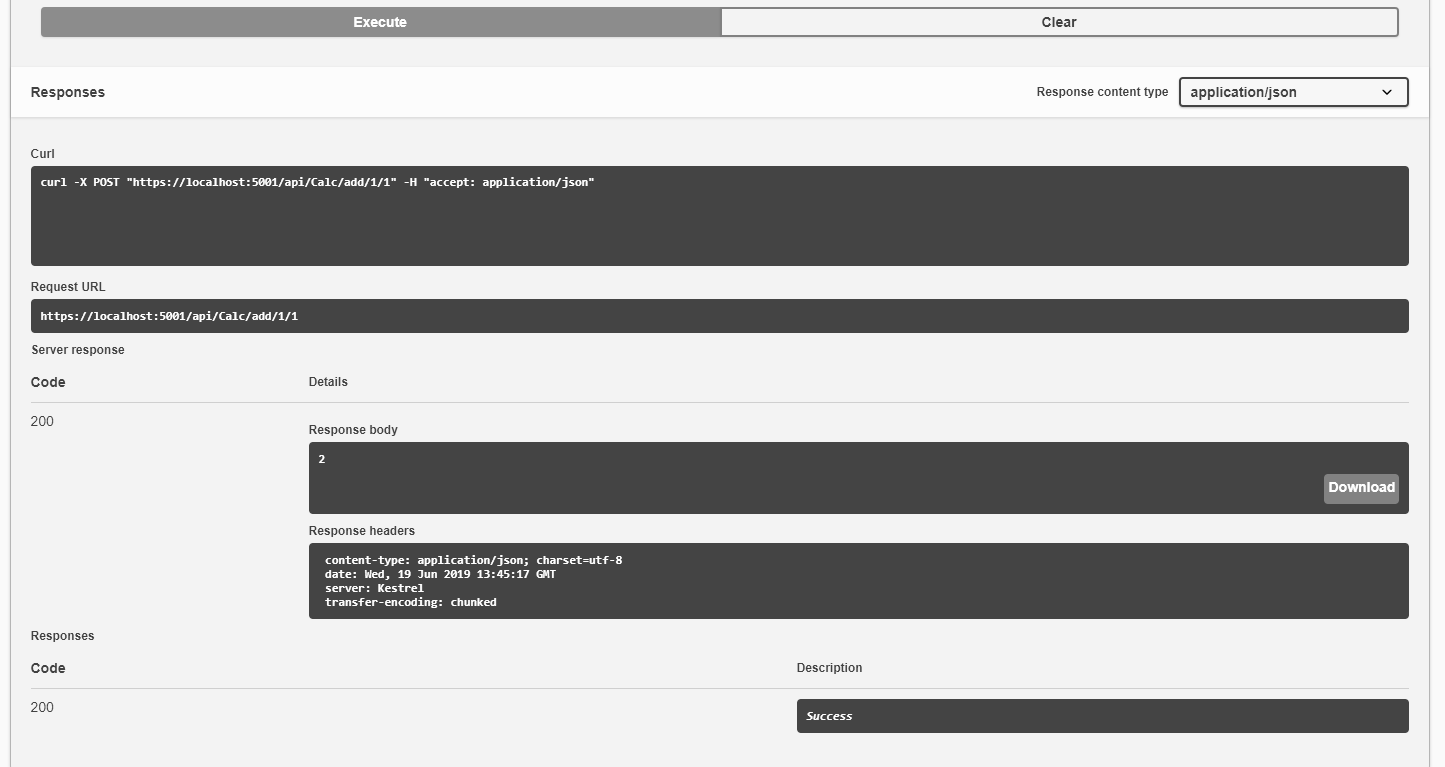
\includegraphics[width=0.8\linewidth]{Cap5/Swagger2.png}
\caption{Interface do \textbf{Swagger} com resposta \textbf{200 OK}}
\label{Fig:Fig49}
\end{figure}

\hspace{1cm}No caso foi retornada a resposta \textbf{200 OK} acompanhada pelo resultado da soma (\ref{Fig:Fig49}). A implementação da funcionalidade que foi desenvolvida, testada, empacotada e instalada na Web API está concluída. 

A próxima fase diz respeito aos testes de integração e performance.

\subsubsection{Criação dos testes de integração e performance}

\hspace{1cm}Os testes de integração e performance serão acompanhados pela criação de uma classe \textit{TestClientProvider}. Esta classe utiliza o servidor de testes da \textbf{Microsoft} -- o \textit{TestServer} -- para simular um cliente que faz pedidos à aplicação. O projeto de teste será criado em \textbf{xUnit} e vai incluir uma referência ao projeto da \textbf{Web API}. À semelhança dos testes unitários, os testes de integração -- que podem ou não incluir testes de performance -- seguem a mesma metodologia, \textit{Triple A}. No entanto, a estrutura dos testes de integração é ligeiramente mais complexa e, caso se pretenda incluir testes de performance, a sua complexidade aumenta. Para a implementação dos testes de integração serviram de apoio as páginas da documentação oficial da \textbf{Microsoft} sobre testes de integração \cite{microsoftintegrationtesting}, o blogue do \textbf{Andrew Lock} \cite{andrewlockblog} e alguns vídeos disponibilizados no canal \textbf{Dot Net Core Central} \cite{dotnetcorecentral} sobre criação de testes de integração.

\subsubsection{Pré-requisitos:}

\begin{itemize}
 \item xUnit (2.4.0);
 \item xUnit.runner.visualstudio (2.4.0);
 \item ModelClasses (1.0.3.4);
 \item FluentAssertions (5.6.0);
 \item Microsoft.AspNetCore.TestHost (2.2.0);
 \item Microsoft.AspNetCore.HttpsPolicy (2.2.0);
 \item Microsoft.AspNetCore.Diagnostics (2.2.0);
 \item Microsoft.AspNetCore.Mvc (2.2.0);
 \item Newtonsoft.Json (12.0.1);
\end{itemize}

\subsubsection{Objetivo dos testes de integração e performance}

\hspace{1cm}Os testes de integração são desenvolvidos quando pretendemos verificar as respostas de um pedido a um determinado \textit{endpoint}. Imaginemos que se pretende testar o comportamento de um método \textbf{POST}, semelhante aquele implementado na \textbf{Web API}, verificando que são efetivamente adicionados os dois números inteiros. Para tal, terá de se verificar que a resposta retornada é do tipo \textbf{200 OK} e que o resultado obtido é igual ao resultado esperado.

\hspace{1cm}Os testes de performance vão ser incluídos na execução dos testes de integração e terão como objetivo medir o seu tempo de execução. É necessário ter em conta que a primeira execução dos testes de integração é sempre mais demorada que as seguintes uma vez que, neste contexto, estará a ser inicializado o servidor de testes antes de ser criado um cliente. 

\begin{figure}[hbt!]
\centering
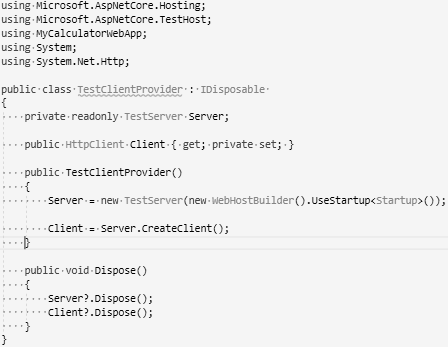
\includegraphics[width=0.7\linewidth]{Cap5/VSTestServer.png}
\caption{Estrutura do \textit{TestClientProvider}}
\label{Fig:Fig50}
\end{figure}

\hspace{1cm}Como dito anteriormente, para simular a criação do cliente utiliza-se a classe \textit{TestServer} que foi desenvolvida pela \textbf{Microsoft}. Desta forma, é criada uma nova classe, dentro do projeto de \textbf{xUnit}, chamada \textit{TestClientProvider} (\ref{Fig:Fig50}). Esta classe vai herdar as propriedades da classe \textit{IDisposable}, vai ter uma propriedade privada do tipo \textit{TestServer} -- que será o  servidor de testes -- e uma propriedade pública do tipo \textit{HttpClient} -- que será o cliente -- cujo objetivo será fazer pedidos à aplicação \textit{MyCalculatorWebApp}. Ainda dentro da classe vão constar dois métodos. O primeiro método será utilizado para criar o servidor de testes com a configuração da classe \textit{Startup.cs} e o cliente que lhe fará pedidos. O segundo método fará \textit{Dispose} ao cliente e ao servidor de testes.



\hspace{1cm}Para ser testada a integração do método \textit{POST}, a \textit{Theory} vai ter apenas um caso de teste -- chamado \textit{TestForResponseTypePOST} (\ref{Fig:Fig51}) -- com três parâmetros inteiros, \textit{n1}, \textit{n2} e \textit{result}. Na fase de \textit{Arrange} será instanciado um novo cliente da classe \textit{TestClientProvider}. De seguida, na fase de \textit{Act}, é dado inicio à contagem do tempo de execução do método \textit{POST} juntamente com o tempo da resposta do servidor. No final, na fase de \textit{Assert}, verifica-se que o tempo demorado é menor do que um valor pré-estabelecido (no caso dois segundos) e depois, com base nessa condição, são feitas duas verificações. É feita uma verificação ao tipo de resposta e outra verificação ao conteúdo da mensagem. Tal como é possível ver na figura \ref{Fig:Fig51}, uma das verificações é feita com o \textit{xUnit} ao passo que a outra é feita em \textit{FluentAssertions}.

\begin{figure}[hbt!]
\centering
\includegraphics[width=0.7\linewidth]{Cap5/VSIntegrationTest.png}
\caption{Estrutura do \textit{TestForResponseTypePOST}}
\label{Fig:Fig51}
\end{figure}

\hspace{1cm}A próxima fase passará pela integração do código da \textbf{Web API} numa \textit{pipeline}, com análise estática e execução de testes de integração. Pode-se ou não integrar as notificações acerca do \textit{status} do \textit{job} com as plataformas de comunicação que a empresa utiliza, neste caso o \textbf{Slack}, mas o principal objetivo é fazer \textit{build} ao projeto da \textbf{Web API} e \textit{restore} às dependências do projeto.

\subsubsection{Configuração do \textit{job}}

\hspace{1cm}Partindo do pressuposto que o código da \textbf{Web API} foi publicado no \textbf{VCS}, serão repetidos os passos realizados na criação do \textit{job} anterior. No \textbf{Jenkins} será criado um \textbf{new item}, do tipo \textit{freestyle job}, podendo ser adicionada uma descrição. Depois será necessário adicionar a ligação ao \textbf{VCS}, a \textbf{GitLab Connection} que foi criada anteriormente, para que seja possível trazer para o \textbf{Jenkins} o código armazenado no repositório (\ref{Fig:Fig52}).

\begin{figure}[hbt!]
\centering
\includegraphics[width=0.9\linewidth]{Cap5/JenkinsGitLabConnection.png}
\caption{Configuração da descrição e do \textit{access token}}
\label{Fig:Fig52}
\end{figure}

\hspace{1cm}Em \textbf{Source Code Management} selecciona-se o repositório \textbf{GitLab} para onde foi publicado o código. Mais uma vez a comunicação entre o sistema de controlo de versões com \textbf{Jenkins} será feita via \textit{SSH}.

\hspace{1cm}Para que o processo de \textit{build} do \textit{job} que está a ser configurado esteja encadeado com o processo de \textit{build} do \textit{job} anterior será preciso fazer-se uma configuração na secção de \textbf{Build Triggers}. Para tal, é necessário selecionar a opção \textit{``Build after other projects are built''} (\ref{Fig:Fig53}) e, como se pretende que apenas seja feito um \textit{trigger} caso a \textit{build} anterior seja bem sucedida, selecciona-se também a opção \textit{``Trigger only if build is stable''}.

\begin{figure}[hbt!]
\centering
\includegraphics[width=0.9\linewidth]{Cap5/JenkinsBuildSecondPipelineAutomatically.png}
\caption{Configuração dos \textit{Build Triggers}}
\label{Fig:Fig53}
\end{figure}

\hspace{1cm}No próximo segmento, em \textbf{Build Environments}, é importante não esquecer de se selecionar a opção de \textit{``Delete workspace before build starts''}, para que seja apagado o \textit{workspace} criado pelo \textbf{Jenkins} antes do início de cada \textit{build}.

\hspace{1cm}Na fase de \textit{build} passa-se à configuração de um conjunto de instruções para integrar a análise estática, a \textit{build} à solução da \textbf{Web API}, a execução dos testes de integração e a interpretação do resultado dos testes, tal como no \textit{job} anterior. À semelhança daquilo que se fez, a integração da análise estática inicia-se através da instrução inicial \colorbox{gray}{\textcolor{white}{\$ dotnet SonarScanner.MSBuild.dll begin /k:``project-key''}} e termina-se com a instrução final \colorbox{gray}{\textcolor{white}{\$ dotnet SonarScanner.MSBuild.dll end}}. A \textit{build} ao projeto é feita com a instrução \colorbox{gray}{\textcolor{white}{\$ dotnet build project-path}} com a adição das opções \colorbox{gray}{\textcolor{white}{-{}-source http://package-source}} onde ``http://package-source'' será o repositório de \textbf{NuGet Packages}. Para se executarem os testes de integração utiliza-se o mesmo \colorbox{gray}{\textcolor{white}{\$ dotnet test project-path -{}-no-build -{}-logger trx}}. Na figura \ref{Fig:Fig54} vêm-se as instruções de \textit{build} à solução assim como de execução dos testes de integração.

\begin{figure}[hbt!]
\centering
\includegraphics[width=0.9\linewidth]{Cap5/JenkinsBuildSecondPipelineBuildSteps.png}
\caption{Configuração dos \textit{Build Steps}}
\label{Fig:Fig54}
\end{figure}

\subsubsection{Integração com \textbf{Slack}}

\hspace{1cm}Para a integração do \textbf{Jenkins} com a plataforma de comunicação interna da empresa -- \textbf{Slack} -- é necessária a instalação do \textit{plugin} \textbf{Slack Notifications} (https://plugins.jenkins.io/slack). 

\hspace{1cm}Do lado do \textbf{Slack} a configuração é relativamente simples. Primeiro é necessário pedir um \textit{token} de acesso à plataforma de comunicação. Isto é feito através do painel de configuração das aplicações \textbf{Slack}. Neste painel (\ref{Fig:Fig55}) pode ser criado o canal com o qual a aplicação -- \textbf{Jenkins CI} -- vai comunicar o estado das \textit{builds} e é também aqui que se gera o \textit{token} de acesso à plataforma de comunicação. 

\begin{figure}[hbt!]
\centering
\includegraphics[width=0.9\linewidth]{Cap5/SlackConfiguration.png}
\caption{Configuração do \textbf{Jenkins CI}}
\label{Fig:Fig55}
\end{figure}

\hspace{1cm}Do lado do \textbf{Jenkins}, como se pode ver na figura \ref{Fig:Fig56}, antes da configuração da \textit{pipeline}, é necessário adicionar o \textit{token} de acesso gerado anteriormente, juntamente com o nome do canal para o qual será transmitida a informação.

\begin{figure}[hbt!]
\centering
\includegraphics[width=0.9\linewidth]{Cap5/JenkinsSlackNotification.png}
\caption{Configuração do \textbf{Slack Notifier}}
\label{Fig:Fig56}
\end{figure}

\hspace{1cm}De seguida, e para finalizar a configuração das \textbf{Slack Notifications}, será necessário voltar ao \textit{job}. No \textit{job} é na fase de \textbf{Post-build Actions} que, para além de serem agregados todos dos resultados da execução dos testes, serão também adicionadas as \textit{Slack Notifications}. Aqui selecionam-se as opções pretendidas, desde notificações de sucesso/insucesso da \textit{build} até a informações sobre os \textit{commits} (\ref{Fig:Fig57}). 

\begin{figure}[hbt!]
\centering
\includegraphics[width=0.9\linewidth]{Cap5/JenkinsPostBuildSlackNotifications.png}
\caption{\textit{Post-build action de \textbf{Slack Notification}}}
\label{Fig:Fig57}
\end{figure}

\hspace{1cm}Nesta fase a \textit{pipeline} contabiliza dois \textit{jobs}. O primeiro \textit{job} encarrega-se da automatização das fases de \textit{build}, \textit{static analysis}, \textit{unit testing}, \textit{packaging} e \textit{push} do módulo de soma para um repositório de artefactos. O segundo \textit{job} encarrega-se das fases de \textit{build}, \textit{static analysis}, \textit{integration testing} e notifica o developer acerca do estado da \textit{build} da \textbf{Web API}. A última fase da \textit{pipeline} envolve a criação de um \textit{job} com o propósito de automatizar a construção e publicação de uma imagem da aplicação. A imagem vai ser criada através de um ficheiro -- \textbf{Dockerfile} -- e a aplicação vai ser publicada através da utilização do \textbf{Docker}.

\subsection{Publicação da Web API}

\hspace{1cm}Para a publicação da aplicação vai ser utilizado o \textbf{Docker}. É através desta tecnologia de orquestração de \textit{containers} que será criada e publicada uma imagem da aplicação com recurso a registo privado de imagens. Com este registo privado podem ser geridas as imagens das aplicações que são criadas sem que mais ninguém tenha acesso. Caso estivessem no registo público do \textbf{Docker}, estariam disponíveis para uso público.

\subsubsection{Criação de um \textit{Dockerfile}}

\hspace{1cm}O \textbf{Dockerfile} é o documento que vai ser utilizado para executar um conjunto de instruções que vão gerar uma versão de \textit{Release} da \textbf{Web API} que foi criada (\ref{Fig:Fig72}). Para a imagem da \textbf{Web API} estar totalmente funcional é necessário copiar os ficheiros \textbf{.csproj} para a \textit{working directory} -- neste caso \textbf{/app} -- para depois resolver as dependências do projeto que estão guardadas no repositório de artefactos. De seguida, a pasta com as dependências resolvidas é copiada para a \textit{working directory}. Depois, novamente a partir da pasta da \textbf{Web API}, é feita \textit{build} à solução com a configuração de \textbf{Release} e com o \textit{output} a ser enviado para a pasta \textbf{/app}. 

\begin{figure}[hbt!]
\centering
\includegraphics[width=0.9\linewidth]{Cap5/DockerfileCalculator.png}
\caption{Estrutura do \textit{Dockerfile}}
\label{Fig:Fig72}
\end{figure}

\hspace{1cm}A partir do resultado da instrução gerada na fase de \textit{build} vai publicar-se o conteúdo gerado para a pasta \textbf{/app} com a configuração de \textit{Release}. Para finalizar, a partir da imagem base, volta-se novamente para a pasta \textbf{/app}, copia-se o conteúdo da instrução anterior (\textit{publish}) para a pasta atual e passa-se o \textit{entrypoint} que é a \textit{dynamically linked library} da \textbf{Web API}.

\hspace{1cm}Após a criação da primeira imagem vai automatizar-se todo o processo de geração da mesma na \textit{pipeline} de integração contínua. Claro está que para tal será necessário recorrer ao \textit{script} gerado anteriormente.

\subsubsection{Criação do job}

\hspace{1cm}O \textit{workflow} inicial do novo \textit{job} é ligeiramente diferente do anterior. Até à fase de \textbf{Build}, não existe qualquer alteração nas configurações. Contudo, quando se executam as instruções necessárias para automatizar o processo de geração, publicação e lançamento da imagem, terão de utilizar-se dois tipos de \textit{build steps} distintos. Até agora têm sido utilizado maioritariamente \textbf{Windows batch command} mas, para este caso, terá de se utilizar \textbf{shell scripts}. 

\subsubsection{Setup do ambiente}

\hspace{1cm}Para o \textbf{setup} ao ambiente irá fazer-se \textit{build} à solução da \textbf{Web API}. À semelhança daquilo que foi feito no \textit{script}, também terá de ser indicada na instrução a \textit{source} dos \textbf{NuGet Packages} (\ref{Fig:Fig73}). O primeiro \textbf{Build step} vai definir o \textit{WORKSPACE} dentro do \textbf{Jenkins}. Com o ambiente definido será necessário entrar na pasta onde está presente o \textbf{Dockerfile}. A instrução para mudar de diretorias no \textbf{Windows} é \colorbox{gray}{\textcolor{white}{\$ cd directory-path}} originado de \textit{change directory}. 

\begin{figure}[hbt!]
\centering
\includegraphics[width=0.9\linewidth]{Cap5/JenkinsBuildModelClassWebApp.png}
\caption{Instrução de \textit{build} à solução}
\label{Fig:Fig73}
\end{figure}

\subsubsection{Criação, publicação e lançamento da imagem da Web API}

\hspace{1cm}Para que se tenha uma ideia de como é gerada, publicada e instanciada uma imagem de \textbf{Docker} é importante que seja lida a documentação sobre estas instruções na página oficial do \textbf{Docker} sobre imagens \cite{dockerimages} e \textit{containers} \cite{dockercontainers}. A sequência cronológica de instruções de publicação de uma aplicação através da utilização de \textbf{Docker CLI} pode ser vista na figura \ref{Fig:Fig74}.

\begin{figure}[hbt!]
\centering
\includegraphics[width=0.9\linewidth]{Cap5/JenkinsGenerateDockerImage.png}
\caption{Criação, publicação e lançamento da imagem da Web API}
\label{Fig:Fig74}
\end{figure}

A imagem da \textbf{Web API} vai ser gerada com uma \textbf{tag} do endereço local do serviço de \textit{registry} seguido pelo seu nome \colorbox{gray}{\textcolor{white}{\$ docker build -t registry-address/image .}}. O servico de \textit{registry} é uma aplicação \textit{server side stateless} escalável que nos permite armazenar e distribuir imagens \textbf{Docker} \cite{dockerregistry}. Existem outras alternativas para armazenamento de imagens, no entanto a implementação implicaria a emissão de um certificado \textbf{SSL self-signed} e para o caso pretende manter-se o processo o mais simples possível.

A próxima instrução será utilizada para colocar a imagem dentro do \textbf{Docker registry}. Para tal, utiliza-se \colorbox{gray}{\textcolor{white}{\$ docker push registry-address/image}} e, para garantir que a instrução funciona corretamente, é necessário verificar que a \textbf{tag} da imagem é igual à \textbf{tag} da instrução anterior. 

De seguida, remove-se a imagem que foi criada na máquina com recurso à instrução \colorbox{gray}{\textcolor{white}{\$ docker image rm registry-address/image}}. Pode ser necessário utilizar a opção \colorbox{gray}{\textcolor{white}{-{}-force}} para que a imagem seja completamente removida do \textbf{Docker} local. Depois, para publicar num \textit{container} a \textbf{Web API} a partir da imagem armazenada no registo, será utilizada a instrução \colorbox{gray}{\textcolor{white}{\$ docker container run [options] image}} juntamente com algumas opções para lançar o \textit{container} na porta \textbf{8123}.

\subsubsection{Pedidos à Web API}

\hspace{1cm}Depois de publicada a imagem vão ser feitos alguns pedidos à aplicação. Para tal, são utilizadas as instruções do \textbf{curl} (https://curl.haxx.se/) tal como pode ser visto na figura \ref{Fig:Fig75}. Para garantir que a aplicação é devidamente publicada e só depois são feitos os pedidos aguarda-se durante 15 segundos com a instrução \colorbox{gray}{\textcolor{white}{\$ sleep 15}}. Só depois são executadas as instruções para os pedidos \textbf{GET} e \textbf{POST} sendo que o \textit{output} pode ser verificado diretamente no \textbf{Jenkins}. 

\begin{figure}[hbt!]
\centering
\includegraphics[width=0.9\linewidth]{Cap5/JenkinsRequestWebAPI.png}
\caption{\textit{Requests} à Web API}
\label{Fig:Fig75}
\end{figure}

\hspace{1cm}Depois de feitos os \textit{requests} e validado o comportamento da \textbf{Web API}, irá ser parado o \textit{container} que foi lançado através da utilização da instrução de paragem \colorbox{gray}{\textcolor{white}{\$ docker container stop container-name}} (\ref{Fig:Fig76}).

\begin{figure}[hbt!]
\centering
\includegraphics[width=0.9\linewidth]{Cap5/JenkinsStopDockerContainer.png}
\caption{Instrução de paragem do \textit{container}}
\label{Fig:Fig76}
\end{figure}

\section{Considerações}

\hspace{1cm}Recapitulando o trabalho feito neste capítulo, que envolveu:

\begin{itemize}
 \item Configuração de um sistema de controlo de versões;
 \item Desenvolvimento um conjunto de testes unitários para validação do funcionamento do módulo de soma;
 \item Configuração um orquestrador de processos (\textbf{Jenkins});
 \item Configuração de um \textit{job} para automatizar as fases de \textit{build}, \textit{static analysis}, \textit{test}, \textit{pack} e \textit{push} de um \textbf{NuGet Package} para um repositório de artefactos;
 \item Descrição do processo de desenvolvimento de uma \textbf{Web API};
 \item Configuração de um \textit{job} para automatizar as fases de \textit{build}, \textit{static analysis}, \textit{integration testing} e notificação do \textit{developer} acerca do estado da \textit{build} e dos detalhes da \textbf{Web API};
 \item Descrição do processo de geração, publicação e lançamento de uma imagem da \textbf{Web API};
 \item Configuração de um \textit{job} para automatizar a fase de \textit{build}, \textit{publish} e \textit{run} da imagem \textbf{Docker} da aplicação;
\end{itemize}

\hspace{1cm}O último passo consiste na criação de um ficheiro de composição dos serviços. Este ficheiro, semelhante ao da figura (\ref{Fig:Fig96}), iria conter dois serviços da \textbf{Web API} que foi criada, com a adição de um serviço de \textit{load balancing} para distribuição dos pedidos. Para fazer a distribuição dos pedidos à aplicação por dois \textit{containers} diferentes foi utilizado como \textit{Web Server} o \textbf{Nginx} (https://www.nginx.com/).

\begin{figure}[hbt!]
\centering
\includegraphics[width=0.43\linewidth]{Cap5/DockerComposeCalculator.png}
\caption{Estrutura do ficheiro \textit{docker-compose.yml}}
\label{Fig:Fig96}
\end{figure}

\hspace{1cm}Em termos de \textit{workflow} a \textbf{Web API} construída incorpora três fases de desenvolvimento. A primeira fase é a fase de \textit{development} onde se desenvolveu o módulo de soma através de práticas de \textbf{TDD}. Os testes são incorporados mais tarde numa \textit{pipeline} de integração contínua, são analisados pelo servidor de automação e, caso sejam bem-sucedidos, é gerado um artefacto daquele módulo que posteriormente será colocado no repositório de artefactos. 

\hspace{1cm}Na fase seguinte o módulo de soma foi utilizado por uma \textbf{Web API} desenvolvida para se verificar que os testes de integração podiam ser feitos através da utilização de uma tecnologia da \textbf{Microsoft}, o \textit{TestServer}. Os testes de integração também testam a performance da aplicação, mas é necessário ter em conta que a primeira execução vai ser sempre mais lenta dado que é necessário inicializar o servidor de testes.

\hspace{1cm}O \textbf{Jenkins} produz depois um \textit{report} detalhado da análise dos testes unitários e de integração que é apresentado ao utilizador para fins estatísticos.

\hspace{1cm}Na terceira fase de desenvolvimento -- a fase de \textit{staging} -- é produzido o \textbf{Dockerfile} que é utilizado para gerar uma imagem. Esta imagem, que no fundo é a versão de \textit{release} (executável) da aplicação, vai ser publicada no registo privado do \textbf{Docker} que foi criado para servir de repositório de imagens. Ainda neste fase, a imagem da aplicação é lançada dentro de um \textit{container} e são feitos dois pedidos à aplicação para verificar que funciona de forma correta. Caso estes pedidos retornem \textit{StatusCodes} diferentes do esperado a aplicação não estará a funcionar como é esperado e requer investigação.

\hspace{1cm}Na última fase -- \textit{Pre-live} -- coloca-se a imagem da aplicação criada, juntamente com uma imagem do \textit{load balancer}, dentro de um ficheiro \textbf{docker-compose.yml}.

\hspace{1cm}O próximo passo é a criação de uma imagem funcional de um serviço composto por uma arquitetura semelhante aquela utilizada pela empresa no desenvolvimento dos seus serviços. Depois da apresentação da solução é ainda apresentado um conjunto de serviços que o \textbf{Docker} disponibiliza.


%-----------------------------------------------------------------------------------------------------------------
%-----------------------------------------------------------------------------------------------------------------
\chapter[Aplicação do protótipo aos serviços da empresa]{Aplicação do protótipo aos serviços da empresa}
\label{Ch:ServicoExemplo}
\section{Serviço de Gestão de tarefas}

\hspace{1cm}Para evidenciar os benefícios da utilização do \textbf{Docker} na orquestração de serviços foi criado um serviço de gestão de tarefas. Este serviço utiliza uma arquitetura base semelhante aquela utilizada pela equipa de desenvolvimento da \textbf{Yugoup} na construção dos serviços quem compõem a plataforma.

\subsubsection{Pré-requisitos}

\begin{itemize}
 \item Microsoft.AspNetCore.App (2.2.0);
 \item Microsoft.AspNetCore.Razor.Design (2.2.0);
 \item Microsoft.EntityFrameworkCore (2.2.4);
 \item Microsoft.EntityFrameworkCore.SqlServer (2.2.4);
 \item Newtonsoft.Json (12.0.2);
 \item Swashbuckle.AspNetCore (4.0.1);
 \item Swashbuckle.AspNetCore.Swagger (1.0.1);
\end{itemize}

\hspace{1cm}Em termos de modelação o serviço de gestão de tarefas tem uma estrutura de dados semelhante à da figura \ref{Fig:Fig85}, com uma tabela \textit{Employee} e outra tabela \textit{Task}. Cada \textit{Employee} pode ter uma ou mais \textit{Tasks} associadas e cada task só pode estar atribuida a um \textit{Employee}.

\begin{figure}[hbt!]
\centering
\includegraphics[width=0.7\linewidth]{Cap7/TimeManagement.png}
\caption{Modelo do Serviço de gestão de tarefas}
\label{Fig:Fig85}
\end{figure}

\subsection{Arquitetura da aplicação}

\hspace{1cm}A arquitetura da aplicação não é 100\% idêntica à arquitetura que a empresa utiliza nos serviços da plataforma \textbf{Yugoup}. No entanto, o objetivo não é replicar um serviço com precisamente a mesma arquitetura do serviço \textit{Tenant}. O objetivo é sim publicar um serviço que inclua as camadas de tratamento de dados que a \textbf{Web API} da calculadora não inclui enquanto se aproxima, em termos de complexidade, do nível de desenvolvimento pretendido. A aplicação está organizada em seis \textit{layers} (\ref{Fig:Fig86}): \textbf{Client SDK, Presentation, Application, Domain, Data} e \textbf{Infrastructure} sendo que as camadas \textbf{Client SDK} e \textbf{Infrastructure} não serão utilizadas. É na camada \textbf{Presentation} que estará contida a API do serviço de gestão de tarefas e é a camada de \textbf{Data} vai modelar a base de dados do serviço. As camadas -- \textbf{Application} e \textbf{Domain} -- são o \textit{middleware} entre as camadas de \textbf{Presentation} e \textbf{Data}.

\hspace{1cm}Não será aprofundado o desenvolvimento do serviço em si, nem é esse o objetivo da apresentação deste serviço. Com a construção deste serviço pretende-se demonstrar que, em termos de conceito, o desenvolvimento com \textbf{Docker} pode ser facilmente integrado nas práticas de qualquer empresa de desenvolvimento de software.

\begin{figure}[hbt!]
\centering
\includegraphics[width=0.5\linewidth]{Cap7/TimeManagementLayers.png}
\caption{Organização do serviço em camadas}
\label{Fig:Fig86}
\end{figure}

\hspace{1cm}Para que possa ser criada uma imagem do \textit{Docker} são necessários os \textit{paths} dos projetos de \textbf{.NET} (\textbf{.csproj}) que compõem a solução. Uma vez que estes projetos estão associados a ficheiros que são utilizados para executar a aplicação, os mesmos terão de estar referenciados algures no \textit{script}. Como se pode ver na figura \ref{Fig:Fig87}, a solução contabiliza um total de cinco destes ficheiros. Os projetos serão utilizados no \textit{Dockerfile}, juntamente com a solução do serviço, para se poder criar uma versão de \textit{Release} da \textbf{Web API} do serviço de gestão de tarefas e assim gerar a versão final de publicação da aplicação.

\begin{figure}[hbt!]
\centering
\includegraphics[width=0.4\linewidth]{Cap7/TimeManagementCSPROJ.png}
\caption{Organização dos projetos}
\label{Fig:Fig87}
\end{figure}

\hspace{1cm}A execução da aplicação a partir do ambiente integrado de desenvolvimento é apresentada no \textit{browser} através da interface gráfica do \textbf{Swagger} (\ref{Fig:Fig88}), que é semelhante à apresentaçaõ do serviço \textit{Tenant}, com os métodos da respetiva \textbf{Web API} do serviço de gestão de tarefas. A interface gráfica comunica com o serviço de armazenamento de dados do \textbf{SQL Server} dentro de um \textit{container}. Este método também foi testado no serviço \textit{Tenant}, como poderá ser visto mais à frente. 

\begin{figure}[hbt!]
\centering
\includegraphics[width=0.8\linewidth]{Cap7/TimeManagementDevelopment.png}
\caption{Interface \textit{Swagger} do serviço de gestão de tarefas}
\label{Fig:Fig88}
\end{figure}

Quando o serviço é inicializado as migrações são feitas para a instância do \textbf{SQL Server} que está a ser executada no \textit{container}, sendo gerada a base de dados \textbf{ServiceTimeManagementContext} com três tabelas (\ref{Fig:Fig89}), \textit{``Employee''}, \textit{``Task''} e \textit{``EFMigrationsHistory''}, a tabela das migrações do \textbf{Entity Framework Core}.

\begin{figure}[hbt!]
\centering
\includegraphics[width=0.35\linewidth]{Cap7/TimeManagementDatabase.png}
\caption{Estrutura da base de dados do \textit{container}}
\label{Fig:Fig89}
\end{figure}

\hspace{1cm}Tal como pode ser visto na figura \ref{Fig:Fig90}, na classe \textit{startup.cs} do serviço de gestão de tarefas, foi adicionado um sufixo ao título da interface gráfica do \textbf{Swagger} com o ambiente atual da aplicação. Neste caso, a aplicação executada a partir do \textbf{IDE} é lançada com as configurações do ambiente de \textbf{Development} (\ref{Fig:Fig88}), \textit{``Time Management ServiceDevelopment''}.

\begin{figure}[hbt!]
\centering
\includegraphics[width=0.9\linewidth]{Cap7/TimeManagementStartupClass.png}
\caption{Estrutura da classe \textit{startup.cs}}
\label{Fig:Fig90}
\end{figure}

\subsection{Criação do \textit{Dockerfile}}

\hspace{1cm}Na criação do \textit{Dockerfile} do serviço foi utilizado o \textit{script} que se pode ver na figura \ref{Fig:Fig91}. A imagem gerada terá a \textbf{tag} do registo seguido do seu nome -- \textbf{localhost:5000/service-time-management} -- e será, mais tarde, publicada no registo privado de imagens.

\begin{figure}[hbt!]
\centering
\includegraphics[width=0.95\linewidth]{Cap7/TimeManagementDockerfile.png}
\caption{Estrutura do script de \textit{Docker}}
\label{Fig:Fig91}
\end{figure}

O serviço de gestão de tarefas, depois de publicado, apresenta o sufixo \textbf{Production} junto ao título (\ref{Fig:Fig92}) uma vez que é este o valor que está definido como variável de ambiente para o \textbf{HostingEnvironment} de \textit{Release}. 

\begin{figure}[hbt!]
\centering
\includegraphics[width=0.9\linewidth]{Cap7/TimeManagementProduction.png}
\caption{Interface \textit{Swagger} do serviço de gestão de tarefa}
\label{Fig:Fig92}
\end{figure}

\subsection{Criação do docker-compose.yml}

\hspace{1cm}A criação de um ficheiro de lançamento da aplicação para \textit{pre-live} vai envolver a execução de quatro \textit{containers}. O primeiro \textit{container} a ser lançado será o da base de dados porque sem ela a aplicação simplesmente não funciona. De seguida são executados dois \textit{containers} com duas aplicações da \textbf{Web API} do serviço de gestão de tarefas, em duas portas diferentes e com \textit{HostingEnvironments} diferentes. Por último lugar, é executado o serviço de \textit{load balancing} da aplicação.

\subsubsection{Serviço de base de dados}

\hspace{1cm}O serviço de base de dados utilizado -- \textbf{MS SQL Server} -- é o primeiro a ser executado e todos os restantes serviços dependem do seu funcionamento. Convém ter em conta que os dois serviços da \textbf{Web API} devem aguardar que a base de dados esteja lançada (\ref{Fig:Fig93}) e devidamente configurada para, só depois, poderem arrancar. Para ultrapassar este problema é necessário garantir que o serviço da \textbf{Web API} só é iniciado depois de ser estabelecida uma conexão ao \textit{container} da base de dados.

\begin{figure}[hbt!]
\centering
\includegraphics[width=0.9\linewidth]{Cap7/TimeManagementDCSQLServer.png}
\caption{Serviço de base de dados da aplicação}
\label{Fig:Fig93}
\end{figure}

Para este caso a solução passou pela implementação de um ciclo de tentativas de conexão ao serviço de base de dados com recurso a um \textit{try-catch}. Como pode ser visto na figura \ref{Fig:Fig99}, no bloco \textit{try} vai ser utilizado o contexto da base de dados que foi configurado para serem feitas as migrações. Enquanto que na cláusula \textit{catch} é feito um ciclo de 10 tentativas de conexão à base de dados.

\begin{figure}[hbt!]
\centering
\includegraphics[width=0.9\linewidth]{Cap7/TimeManagementCheckDBService.png}
\caption{Verificação da configuração do Serviço de Base de dados}
\label{Fig:Fig99}
\end{figure}

\subsubsection{Serviço de Web API}

\hspace{1cm}Os dois serviços da \textbf{Web API} dependem do serviço de BD para poderem funcionar. O serviço \textit{time-management-api1} apresenta a variável de ambiente com a configuração de \textit{Release} por defeito. Já o serviço \textit{time-management-api2} apresenta uma variável de ambiente diferente ao utilizador apesar de ter a mesma configuração de \textit{Release} do seu par. Como se pode ver pela figura \ref{Fig:Fig94}, nas variáveis de ambiente \textbf{time-management-api2}, o valor de \textit{HostingEnvironment} daquela instância é definido como \textit{``Test''} através da utilização da variável de ambiente \textbf{ASPNETCORE\_ENVIRONMENT=Test}. Assim sendo, quando for utilizado o \textit{load balancer} para distribuir os pedidos pelas duas \textbf{Web APIs} sabe-se, através do sufixo apresentado no título, qual a instância da API que está a ser apresentada no \textit{browser}. 

\begin{figure}[hbt!]
\centering
\includegraphics[width=0.45\linewidth]{Cap7/TimeManagentDCWebAPI.png}
\caption{Serviço de apresentação da \textbf{Web API}}
\label{Fig:Fig94}
\end{figure}

\subsubsection{Serviço de \textit{Load Balancing}}

\hspace{1cm}Da mesma forma que os serviços da \textbf{Web API} dependem do serviço de base de dados para poderem ser inicializados, os serviço de \textit{load balancing} vai esperar que as duas APIs estejam lançadas para poder ser executado. Pela figura \ref{Fig:Fig95} pode verificar-se que o \textbf{nginx} é o último serviço a ser executado.

\begin{figure}[hbt!]
\centering
\includegraphics[width=0.45\linewidth]{Cap7/TimeManagementLoadBalancing.png}
\caption{Serviço de \textit{load balancing}}
\label{Fig:Fig95}
\end{figure}

\hspace{1cm}Após a fase de \textit{development}, os passos para a publicação de um serviço repetem-se sistematicamente. A seguir à criação das imagens que vão compor o serviço nas fases de \textit{pre-live} e \textit{production}, é sempre produzido um ficheiro de composição \textbf{(docker-compose.yml)} que vai orquestrar a publicação da aplicação, serviço a serviço, pela sequência cronológica de instruções de publicação que lhe são transmitidas.

\subsection{Considerações}

\hspace{1cm}Este tipo de metodologia de publicação pode ser utilizado localmente ou online, com uma condição. Na máquina onde o serviço é publicado, terá de estar instalado o \textbf{Docker}.

\hspace{1cm}Caso o serviço esteja publicado em rede local, como por exemplo, na máquina de \textit{staging} disponibilizada pela empresa, os custos de operação passam a ser única e exclusivamente a energia consumida pela máquina, contrariamente ao que acontece quando um serviço é publicado online para ser testado. Uma das principais vantagens é a facilidade com que se consegue replicar toda a infra-estrutura, o que facilita não só o desenvolvimento em si, mas também a \textit{pipeline} de teste, porque desta forma é possível criar e destruir os ambientes facilmente.

\hspace{1cm}Um dos contratempos da utilização do \textbf{Docker} (versão do \textbf{Windows}) é a perda de dados em situações como, por exemplo, quando uma máquina é reiniciada sem existir persistência de dados. Estes dados nunca mais serão recuperados, uma vez que por definição os \textit{containers} são voláteis. Assim sendo, para contornar este problema é necessário utilizar \textit{containers} para guardar os dados das aplicações que estão a ser utilizadas, e utilizar os seus volumes como repositórios de dados. Desta forma os dados ficarão sempre persistidos na memória dos outros \textit{containers}, mesmo que o serviço do \textbf{Docker} falhe inesperadamente.

\hspace{1cm}Os próximos passos serão a implementação de uma \textit{pipeline} de integração e entrega contínua para um serviço da plataforma Yugoup. Para tal, será criada uma \textit{branch} paralela à \textit{Master} -- chamada \textbf{cicd} -- que permitirá trabalhar em conformidade com os objetivos estabelecidos pela equipa de orientação sem interferir com os desenvolvimentos da equipa da empresa. O serviço mais importante da plataforma, o \textit{Tenant}, foi o escolhido para percorrer todas as fases de integração contínua.

\section{Plataforma Yugoup}
\label{Ch:Plataforma Yugoup}

\hspace{1cm}A plataforma de comércio eletrónico \textbf{Yugoup} foi desenvolvida segundo o estilo de arquitetura orientada a serviços (por camadas) e contabiliza 36 serviços, no momento de escrita do documento. A arquitetura dos serviços é constituída por 6 camadas -- \textit{top-to-bottom:} \textbf{Client SDK, Presentation, Application, Domain, Data} e \textbf{Infrastructure} -- e inclui testes unitários às camadas de \textbf{Application, Domain} e \textbf{Data}. Para esta fase, o objetivo seria construir uma \textit{pipeline} de testes automatizada. Os desafios seriam a integração de análise estática e o desenvolvimento de testes de integração e performance num serviço disponibilizado, mais concretamente na camada de \textbf{Presentation}. 

\hspace{1cm}A empresa disponibilizou um serviço (\textit{Tenant}) para integração continua numa \textit{pipeline} de testes automatizada com a execução dos testes unitários pré-existentes. Os serviços foram publicados, pela equipa da \textbf{Yugoup} numa máquina, em rede local, dentro do espaço de trabalho o que significa que os testes de integração e performance seriam feitos diretamente contra o serviço \textit{t-yugoup-tenant} publicado em \textit{staging}.

\subsection{Integração contínua do serviço \textit{Tenant}}

\hspace{1cm}Os testes de integração e performance serão desenvolvidos e integrados, juntamente com a análise estática ao código, na instância do \textbf{Jenkins} previamente instalada e configurada na máquina de \textit{staging}.

\subsection{Desenvolvimento dos testes de integração e performance}

\hspace{1cm}Foram desenvolvidos quatro testes de integração e dois testes de performance ao serviço \textit{Tenant}. Como é possível ver na figura \ref{Fig:Fig58}, os testes de integração utilizam uma classe -- \textbf{ClientExtensions} -- cuja função é criar o cliente. Esta classe contém um método -- \textbf{CreateClient} -- que recebe como parâmetro uma \textit{string}. Essa \textit{string} é o \textbf{URL} do serviço do \textit{Tenant} que foi publicado localmente em \textit{staging}.

\begin{figure}[hbt!]
\centering
\includegraphics[width=0.9\linewidth]{Cap6/TenantClientExtensions.png}
\caption{Classe \textit{ClientExtensions}}
\label{Fig:Fig58}
\end{figure}

\hspace{1cm}O primeiro teste de integração foi criado para testar a existência do \textbf{GUID} -- \textit{Global Unique Identifier} -- que é gerado automaticamente quando são feitas as migrações, logo após a criação das bases de dados. O cliente gera um \textit{token} de autenticação para o \textbf{Tenant} e as verificações são feitas ao tipo de resposta e ao conteúdo da mensagem (\ref{Fig:Fig59}).

\begin{figure}[hbt!]
\centering
\includegraphics[width=0.9\linewidth]{Cap6/TenantDefaultGUID.png}
\caption{Teste à presença do \textit{Default GUID}}
\label{Fig:Fig59}
\end{figure}

\hspace{1cm}O segundo teste de integração foi criado para testar um GUID inexistente. O cliente gera um \textit{token} de autenticação para o \textbf{Tenant} e as verificações são feitas ao tipo de resposta e ao conteúdo da mensagem (\ref{Fig:Fig60}) à semelhança do teste anterior.

\begin{figure}[hbt!]
\centering
\includegraphics[width=0.9\linewidth]{Cap6/TenantMissingGUID.png}
\caption{Teste à presença de um \textit{GUID} inexistente}
\label{Fig:Fig60}
\end{figure}

\hspace{1cm}O terceiro teste de integração tem uma componente de teste à performance na medida em que é testado o tempo de resposta do pedido de acesso à aplicação com a \textit{property} \textbf{enabled=true} presente na mensagem (\ref{Fig:Fig61}).

\begin{figure}[hbt!]
\centering
\includegraphics[width=0.9\linewidth]{Cap6/TenantAuthorization.png}
\caption{Teste de acesso autorizado}
\label{Fig:Fig61}
\end{figure}

\hspace{1cm}O quarto teste de integração tem uma componente de teste à performance, semelhante ao teste anterior, na medida em que é testado o tempo de resposta do pedido de acesso à aplicação sem a \textit{property} \textbf{enabled=true} presente na mensagem (\ref{Fig:Fig62}).

\begin{figure}[hbt!]
\centering
\includegraphics[width=0.9\linewidth]{Cap6/TenantUnauthorized.png}
\caption{Teste de acesso não autorizado}
\label{Fig:Fig62}
\end{figure}

\hspace{1cm}Os testes estão todos organizados de forma a que as \textit{Assertions} sejam feitas ao tipo de resposta esperado, portanto todos os testes foram validados. O próximo desafio é alinhar os testes de integração/performance com todos os testes unitários já existentes. Para tal, na \textit{pipeline} serão necessários todos os serviços com os quais o \textbf{Tenant} comunica.

\subsection{\textit{Pipeline}}

\hspace{1cm}Os serviços da plataforma que estão referenciados no projeto do serviço \textit{t-yugoup-tenant} são necessários para que o projeto possa ser devidamente integrado na \textit{pipeline}. Quer isto dizer que, para que seja possível compilar o código do projeto, seria também necessário integrar na \textit{pipeline} o código de todos os projetos com os quais o \textit{Tenant} tem dependências ou referências. Será portanto necessário gerir vários repositórios e incluir todas as soluções das dependências do projeto numa pasta, que posteriormente será reorganizada, e só depois poderão ser feitas as operações sobre o código. De seguida será então possível integrar análise estática, restaurar as dependências do projeto do serviço \textit{Tenant}, fazer \textit{build} ao projeto, executar testes unitários, testes de integração/performance e, por fim, interpretar os resultados dos testes. Foi também necessário instalar um \textit{plugin} para que se possam analisar vários repositórios em simultâneo.

\hspace{1cm}Para o \textit{setup} do ambiente do \textbf{Jenkins} foi utilizado um \textit{script} semelhante ao da figura \ref{Fig:Fig63}. Este \textit{script} vai criar uma pasta (final) e uma subpasta (src), vai fazer \textit{clone} aos repositórios que fazem parte da plataforma e, por fim, \textit{build} ao projeto. Isto acontece porque, como dito anteriormente, são necessários todos projetos da plataforma \textit{Yugoup}, que estão referenciados no projeto \textit{t-yugoup-tenant}, para que possa ser feita \textit{build} ao serviço da \textbf{Web API} do \textit{Tenant}.

\begin{figure}[hbt!]
\centering
\includegraphics[width=0.9\linewidth]{Cap6/SetupEnvScript.png}
\caption{\textit{Script} de \textit{setup}}
\label{Fig:Fig63}
\end{figure}

\hspace{1cm}No \textbf{Jenkins}, dá-se uma descrição à \textit{pipeline}. Em \textbf{Source Code Management}, selecciona-se o \textit{plugin} \textbf{Multiple SCMs} e configura-se a ligação aos repositórios via \textbf{SSH}. Todos os repositórios que vão ser adicionados à \textit{pipeline} vão seguir a mesma metodologia. Primeiro será inserido o \textbf{URL} do repositório e é seleccionada a credencial de acesso por \textbf{SSH} e só depois é especificada a \textit{branch} sob a qual serão feitas as operações. Por fim, dá-se um nome à pasta onde serão colocados os ficheiros dos projetos (\ref{Fig:Fig64}). As configurações restantes serão idênticas, não existirão \textbf{Build Triggers}, apenas será eliminado o \textit{workspace} antes de cada \textit{build}. 

\hspace{1cm}Em \textbf{Build}, todos os \textit{build steps} utilizados para criar o \textit{setup} serão feitos à semelhança do \textit{script} que se pode visualizar na figura \ref{Fig:Fig63}. À semelhança do \textit{script}, como dito anteriormente, foi criada um diretoria -- final -- e uma subdiretoria -- \textbf{src} -- para onde foram passados os ficheiros dos serviços. Foi utilizado o \textbf{robocopy} para copiar os ficheiros para a subdiretoria: \colorbox{gray}{\textcolor{white}{\$ robocopy project-name folder-path}} juntamente com as opções \colorbox{gray}{\textcolor{white}{/COPYALL /e /NFL /NDL /NJH  /nc /ns /np}} \cite{robocopy}.

\begin{figure}[hbt!]
\centering
\includegraphics[width=0.9\linewidth]{Cap6/JenkinsMultipleSCM.png}
\caption{\textit{Multiple Source Code Management}}
\label{Fig:Fig64}
\end{figure}

\subsubsection{Fase de \textbf{Build} do projeto}

\hspace{1cm}As primeiras instruções na fase de \textit{build} do projeto \textit{tenant} são a instrução de arranque da análise estática e a instalação dos \textbf{NuGet Packages} presentes num repositório online. Posteriormente é feita \textit{build} à solução do \textit{Tenant} (\ref{Fig:Fig65}).

\begin{figure}[hbt!]
\centering
\includegraphics[width=0.9\linewidth]{Cap6/JenkinsTenantBuild.png}
\caption{Análise estática, \textit{Restore} e \textit{Build} }
\label{Fig:Fig65}
\end{figure}

\hspace{1cm}Para iniciar a análise estática foram repetidos os passos do capítulo anterior. Depois de iniciada a análise estática e antes e antes de ser feita \textit{build} à solução é executado um \textit{script} que vai instalar todas as dependências através da utilização de um ficheiro \textbf{batch} (.bat) desenvolvido pela equipa da \textbf{Yugoup}. Na fase de \textit{build} da solução -- e após o \textit{setup} do ambiente -- todas as soluções serão revistas pela análise estática. Isto acontece porque se está a fazer \textit{build} à solução do \textit{Tenant} em conjunto com as soluções das suas dependências.

\subsubsection{\textit{Build} e \textit{Run} dos testes unitários}

\hspace{1cm}Também à semelhança daquilo que foi feito no capítulo anterior, os testes unitários terão de ser compilados (\ref{Fig:Fig66}) e executados (\ref{Fig:Fig67}) para que sejam gerados resultados. Só depois se podem armazenar e apresentar estes resultados. O mesmo acontece com os testes de integração e performance.

\begin{figure}[hbt!]
\centering
\includegraphics[width=0.9\linewidth]{Cap6/TenantUnitTests.png}
\caption{Compilação dos projetos de teste}
\label{Fig:Fig66}
\end{figure}

\begin{figure}[hbt!]
\centering
\includegraphics[width=0.9\linewidth]{Cap6/TenantUnitTestsExecution.png}
\caption{Execução dos projetos de teste}
\label{Fig:Fig67}
\end{figure}

 As instruções de execução dos testes já são conhecidas e, como pode ser visto pela figura (\ref{Fig:Fig68}), antes da execução dos testes de integração é necessário executar outro \textit{script}, através de um ficheiro \textbf{batch} (.bat), para remover o \textit{feed} das dependências do projeto. Resta parar a execução da análise estática e pode então proceder-se à execução dos testes de integração e performance.


\begin{figure}[hbt!]
\centering
\includegraphics[width=0.9\linewidth]{Cap6/TenantRemoveFeed.png}
\caption{Remoção das dependências}
\label{Fig:Fig68}
\end{figure}

\subsubsection{\textit{Build} e \textit{Run} dos testes integração e performance}

\hspace{1cm}Os testes de integração e performance são compilados e executados (\ref{Fig:Fig69}) à semelhança dos testes unitários. Na fase de \textbf{Post-build Actions} vão interpretar-se os resultados de todos os testes em simultâneo. 

\begin{figure}[hbt!]
\centering
\includegraphics[width=0.9\linewidth]{Cap6/TenantIntegrationTests.png}
\caption{Compilação e execução dos testes de integração e performance}
\label{Fig:Fig69}
\end{figure}

\hspace{1cm}Um complemento interessante à \textit{pipeline} seria a geração automática de uma imagem de \textbf{Docker} do serviço \textbf{t-yugoup-tenant}. A imagem foi gerada e exposta numa porta pública mas o seu processo de geração não foi incluído na \textit{pipeline}. Apesar da aplicação ter sido publicada, o seu endereço não estava autorizado a aceder aos serviços da plataforma Yugoup. Em baixo é apresentada a estrutura do \textit{Dockerfile} que deu origem à imagem do serviço e são delineados um conjunto de \textbf{Next Steps} para o futuro, caso a equipa pretenda integrar na \textit{pipeline} o processo de geração automática da imagem através de um \textit{Dockerfile}.

\subsection{Geração da imagem do serviço \textit{Tenant}}

\hspace{1cm}A versão de \textit{Release} da \textbf{Web API} do serviço \textit{Tenant} sobre a qual estão a ser feitos os testes de integração foi publicada na máquina de \textit{staging} através de \textbf{Web Deploy} \cite{webdeployiis}. Contudo, seria interessante publicar uma imagem de \textbf{Docker} do serviço \textit{Tenant} semelhante à imagem da \textbf{Web API} da Calculadora. 

\hspace{1cm}Foram incluídos todos os projetos (\ref{Fig:Fig77}) que compõem o serviço \textit{Tenant} e foi feito \textit{restore} a partir do repositório de artefactos que foi disponibilizado pela equipa do projeto (\ref{Fig:Fig78}). De seguida foi copiada a pasta de configuração do ficheiro \textbf{NuGet.config} para a pasta \textbf{/app}, foram executadas as intruções de \colorbox{gray}{\textcolor{white}{\$ dotnet build}} e \colorbox{gray}{\textcolor{white}{\$ dotnet publish}} (\ref{Fig:Fig79}) com a configuração de \textit{Staging} e o \textit{output} a ser colocado na pasta \textbf{/app}. Por fim foi publicada a aplicação com a \textit{dynamically linked library} da \textbf{Web API} do serviço de \textit{Tenant} tal como pode ser visto na figura \ref{Fig:Fig79}.

\begin{figure}[hbt!]
\centering
\includegraphics[width=0.9\linewidth]{Cap6/TenantDockerfileCSPROJ.png}
\caption{Dockerfile do serviço \textit{Tenant}}
\label{Fig:Fig77}
\end{figure}


\begin{figure}[hbt!]
\centering
\includegraphics[width=0.9\linewidth]{Cap6/TenantDockerfileNuGetConfig.png}
\caption{Dockerfile do serviço \textit{Tenant}}
\label{Fig:Fig78}
\end{figure}

\begin{figure}[hbt!]
\centering
\includegraphics[width=0.9\linewidth]{Cap6/TenantDockerfilePublish.png}
\caption{Dockerfile do serviço \textit{Tenant}}
\label{Fig:Fig79}
\end{figure}

\hspace{1cm}Sem alterar o código da plataforma, uma vez que não eram permitidas alterações à sua base, e sem interferir com os tipos de bases de dados que a plataforma está a utilizar, foi criada uma base de dados do mesmo tipo que o serviço utiliza -- \textbf{SQL Server} -- através do uso de uma imagem de \textbf{Docker} disponibilizada no repositório oficial que a \textbf{Microsoft} criou para imagens do \textbf{Microsoft SQL Server} \cite{dockersqlserver}. Também é necessário fazer uma pequena alteração à \textit{connection string} do serviço \textit{Tenant} uma vez que terá de ser ligeiramente diferente daquela que o serviço que está publicado na máquina de \textit{staging} utiliza atualmente para que a base de dados a ser executada dentro de um \textit{container} possa ser acedida e manipulada. 

    \hspace{1cm}Tal como é apresentado na figura \ref{Fig:Fig80}, pode ser vista a \textit{connection string} de ligação ao \textit{container} do \textbf{Docker} onde está a ser executada a imagem do \textbf{SQL Server}. Comentada, na linha anterior, também pode ser vista a \textit{string} de ligação à base de dados antiga. Para verificar que a base de dados de \textbf{SQL Server está a funcionar} é necessário aceder ao \textit{container} via \textbf{Azure Data Studio}. São assim necessárias as credenciais de acesso com as quais foi lançado o serviço de base de dados e é necessário colocar no campo \textbf{Server}: \textit{localhost, port-number} (\ref{Fig:Fig81}). Quando a conexão à base de dados for estabelecida será possível ver uma luz verde (semelhante à da figura \ref{Fig:Fig83}) ao lado do nome da base de dados e, depois de se iniciar o serviço do tenant, poderá ser então vista a base de dados criada pelo \textbf{EF Core} -- \textbf{TenantRepository} -- dentro da diretoria das bases de dados.

\begin{figure}[hbt!]
\centering
\includegraphics[width=0.9\linewidth]{Cap6/TenantConnectionString.png}
\caption{\textit{Connection String} da Base de Dados}
\label{Fig:Fig80}
\end{figure}

\begin{figure}[hbt!]
\centering
\includegraphics[width=0.4\linewidth]{Cap6/MSSQLServerTenantRepository.png}
\caption{Conexão ao serviço de base de dados pelo \textbf{Azure Data Studio}}
\label{Fig:Fig81}
\end{figure}

\hspace{1cm}A imagem do serviço foi depois publicada com a \textit{tag} \textbf{t-yugoup-tenant} e posteriormente foi lançado um \textit{container} com o projeto da \textbf{Web API} que mais tarde foi acedido pelo \textit{browser}.

\subsection{Resultados}

\hspace{1cm}A apresentação dos resultados dos testes e da análise estática vai ser o produto final da \textit{pipeline} de testes automatizada. 

\subsubsection{Apresentação dos resultados dos testes}

\hspace{1cm}A apresentação dos resultados dos testes no \textbf{Jenkins} é feita com um gráfico. Este gráfico contém o número de testes -- \textit{Passed, Failed e Skipped} -- no eixo dos \textbf{y} e o número da \textit{build} no eixo dos \textbf{x}. 
Na figura \ref{Fig:Fig70} são apresentados os resultados dos testes, na sua maioria, por um tom de cinza intermédio.

\begin{figure}[hbt!]
\centering
\includegraphics[width=0.9\linewidth]{Cap6/TenantTestResults.png}
\caption{Resultado dos testes}
\label{Fig:Fig70}
\end{figure}

Quer isto dizer que grande parte dos testes são executados com sucesso. Na \textit{build} número 187 foi introduzida a análise aos quatro testes de integração, dois dos quais com testes de performance, cujo resultado inicial da execução não foi de encontro ao esperado, sendo possível ver pela cor cinza escuro. No entanto duas \textit{builds} depois (189) os testes foram compilados e executados com sucesso, o que resultou numa subida no número total de testes \textit{Passed}. Para ser vista a representação dos testes \textit{Skipped} foi criado, a título de exemplo, um teste unitário em \textbf{MSTest} com o atributo \textbf{Skip} -- representado a cinza claro -- para ser conhecida a sua interpretação gráfica. 

\hspace{1cm}No total, o serviço do \textbf{Tenant} contabiliza dezoito testes. Destes dezoito testes, um é passado à frente (\textit{Skipped}). Quatro desses dezoito testes são testes feitos à integração dos \textit{endpoints} da plataforma e dois desses quatro testes são testados em termos de performance. Os restantes treze testes são testes unitários, feitos às camadas de manipulação e tratamento de dados da plataforma.

\subsubsection{Resultados da análise estática}

\hspace{1cm}A análise estática apresentou um conjunto alertas relativos a falhas de segurança, \textit{bugs}, \textit{Code Smells} e vulnerabilidades dentro da plataforma, no entanto o \textbf{quality gate} foi positivo, como é possível verficar-se na figura \ref{Fig:Fig71}.

\hspace{1cm}Foram identificados 27 \textit{Bugs}, 37 \textit{Vulnerabilities}, 634 \textit{code smells} e 193 \textit{Security Hotspots}. Em termos de gravidade, foram identificados 5 \textit{Issues} do tipo \textit{Blocker}, 198 do tipo \textit{Minor}, 105 do tipo \textit{Critical}, 385 do tipo \textit{Major} e 5 do tipo \textit{Info}. Toda a informação acerca dos \textit{Issues} identificados pela análise estática do \textbf{Sonarqube} é descrita em detalhe na documentação oficial \cite{sonarqubetooldocs}.

\begin{figure}[hbt!]
\centering
\includegraphics[width=0.9\linewidth]{Cap6/TenantStaticAnalysis.png}
\caption{\textit{Overview} da análise estática}
\label{Fig:Fig71}
\end{figure}

\subsection{Considerações}

\hspace{1cm}Após a conclusão da execução da \textit{pipeline} verificamos que o serviço do \textit{Tenant} está validado com uma bateria de testes e com a análise estática. Numa primeira fase, depois da junção de todos os projetos numa pasta final, é executada análise estática. Inicialmente a análise estática iria ser executada contra o serviço do \textit{Tenant}. No entanto, apesar da \textit{build} ser feita apenas ao serviço que pretendíamos analisar inicialmente, todos os projetos que estão dependentes do serviço vão ser analisados. Como muitos projetos dependem, direta ou indiretamente, do serviço do \textit{Tenant} vamos ter a plataforma \textbf{da Yugoup} analisada por completo. Apesar de ir contra o objetivo inicial, a análise estática faz mais do que aquilo que inicialmente foi estabelecido. A análise estática é fundamentalmente uma análise léxica e sintática do código desenvolvido pela equipa da Yugoup. É possível afirmar também que a análise estática pode incorporar análise semântica tendo em conta o contexto do negócio. Do ponto de vista funcional, o \textbf{Sonarqube} é incluído na \textit{pipeline} porque é fundamental que todo o código seja revisto e analisado de acordo com as boas práticas de programação e para que seja verificado que não existem variáveis, métodos ou chamadas de funções não implementados ou não utilizados dentro da plataforma.

\hspace{1cm}A execução dos testes unitários é importante do ponto de vista semântico e de compilação. Com os testes unitários, são feitas verificações ao modelo da aplicação que é testado de acordo com um conjunto de especificações, tendo em conta as funcionalidades implementadas, as quais foram pedidas com regras pelo \textit{business}. Os testes unitários também procuram testar se essas mesmas regras são aplicadas e se os resultados obtidos vão de encontro aos resultados esperados.

\hspace{1cm}Os testes de integração e performance são utilizados para testar a integração entre serviços através da comunicação com \textit{endpoints} na máquina de \textit{staging}. Junto com testes de integração, são aproveitados os tempos de resposta, tempos esses que são -- após execução dos testes -- dados como testes de performance.

\begin{figure}[hbt!]
\centering
\includegraphics[width=0.9\linewidth]{Cap6/TenantScreenShot.png}
\caption{\textit{Screenshot} do serviço \textit{Tenant} executado a partir do IDE}
\label{Fig:Fig83}
\end{figure}

\begin{figure}[hbt!]
\centering
\includegraphics[width=0.9\linewidth]{Cap6/TenantServiceNotRespondingScreenShot.png}
\caption{\textit{Screenshot} do serviço \textit{Tenant} executado a partir da imagem \textbf{Docker}}
\label{Fig:Fig84}
\end{figure}

\hspace{1cm}O \textit{Tenant} funciona como esperado quando executado a partir do ambiente integrado de desenvolvimento (\ref{Fig:Fig83}). Mesmo com a base de dados de \textbf{SQL Server} servida a partir do \textit{container}. Por outro lado, o comportamento do serviço \textit{Tenant}, quando executado a partir da imagem gerada anteriormente através do \textit{Dockerfile} -- que pode ser visualizado nas figuras \ref{Fig:Fig77}, \ref{Fig:Fig78} e \ref{Fig:Fig79} -- é diferente  (\ref{Fig:Fig84}) do esperado. O problema apresentado é uma medida de segurança, a qual pode ser descativada, que foi implementada para proibir interações que não estejam configuradas ou esperadas. Esta medida de segurança usa-se para colocar um serviço por detrás de um \textit{Gateway}, o qual é o único a ter acesso a essa API. A configuração garante que apenas e só -- e só mesmo -- o serviço \textit{Gateway} consegue comunicar com esses serviços. Este mecanismo apresenta também a vantagem de prevenir \textbf{DDoS} pois, em termos de \textit{stack} de chamada, faz com que o pedido falhe imediatamente sem ocupar grande quantidade de recursos.

\section{Integração de sistemas de visualização}
\label{Ch:CapExemplo}

\hspace{1cm}Como forma de obter feedback mais rápido acerca do resultado da \textit{pipeline} surgiu a necessidade de implementação de um sistema de visualização integrado no ciclo de desenvolvimento e teste de software. O principal objetivo da integração deste sistema de visualização seria a colocação do estado de uma \textit{build} num monitor LCD disponibilizado pela empresa. O sistema servirá para notificar os \textit{developers} acerca do estado das \textit{builds} e estará ligado, em rede local, à máquina de  \textit{staging} que, por sua vez, conta com uma instância do \textit{Jenkins} pronta a executar um conjunto de \textit{Jobs}.

\subsection{Sistema de visualização}

As especificações do sistema, em termos de requisitos funcionais, seriam as seguintes: 

\begin{itemize}
  \item O sistema deve apresentar o resultado final de uma \textit{build};
  \item O sistema deve notificar os \textit{developers};
  \item O sistema deve utilizar o LCD disponibilizado pela empresa;
  \item O sistema deve utilizar um Raspberry PI;
  \item O sistema deve estar conectado à rede local;
\end{itemize}

\hspace{1cm}Para além da monitorização -- quase instantânea -- dos \textit{jobs}, o sistema de visualização estará disponível via FTP \textit{(File Transfer Protocol)}. Isto permitirá a inclusão de um conjunto de ficheiros, como os ficheiros com as credenciais de acesso à máquina de \textit{staging}, para facilitar a conexão ao sistema central.

\subsection{Integração do sistema de visualização}

\hspace{1cm}Para a integração de um sistema idêntico de visualização em rede -- local ou online -- é necessário que o sistema central conte com:

\begin{itemize}
  \item Uma instância do \textbf{\textit{Jenkins}};
  \item O \textit{Plugin} \textbf{\textit{Build Monitor}};
  \item Um \textbf{\textit{Job}};
\end{itemize}

\hspace{1cm}Para a integração do sistema de visualização vão ser necessários:

\begin{itemize}
  \item Um \textbf{\textit{Raspberry PI}}, com o respetivo carregador;
  \item Um \textbf{\textit{SD Card}} com, pelo menos, 8GB de memória;
  \item Um teclado;
  \item Um rato ótico (opcional);
  \item Um monitor, como referido anteriormente;
  \item Um cabo de rede;
  \item Um cabo HDMI;
\end{itemize}

\subsection{Instalação do sistema de visualização}

\hspace{1cm}O primeiro passo para que seja possível integrar o sistema de visualização no ciclo de desenvolvimento de software é a formatação do cartão de memória que irá conter o sistema operativo do mini-computador, o \textbf{\textit{Raspberry PI}}. Para a formatação do \textbf{\textit{SD Card}} existem vários softwares disponíveis mas, neste caso, foi utilizado o software \textbf{\textit{SD Card Formatter}}.

\hspace{1cm}De seguida, procede-se à instalação do sistema operativo no \textbf{\textit{SD Card}} pré-formatado. No site oficial da \textbf{Raspberry} são disponibilizados vários sistemas operativos, juntamente com um instalador de sistemas operativos, na secção de downloads. Neste caso, foi utilizado o \textbf{\textit{NOOBS}} (\textit{New Out-of-the Box Software}), que é um instalador de sistemas operativos \textit{user-friendly}.

\subsection{Configuração do sistema de visualização}

\hspace{1cm}Para proceder à configuração do sistema de visualização certifica-se, primeiramente, que o dispositivo contém uma fonte de alimentação com a potência adequada. Após essa verificação, conecta-se o teclado, o rato (caso se disponha de um), o cabo HDMI e o cabo de rede. Antes de se proceder à primeira execução do dispositivo, insere-se o \textbf{\textit{SD Card}} na parte inferior do \textbf{\textit{Raspberry PI}} com o instalador de sistemas operativos, ou com a imagem do sistema operativo que vai ser utilizado. Só depois de se completar os passos anteriores é ligado o dispositivo à corrente. Se todos os passos tiverem sido devidamente executados, o sistema de configuração do dispositivo deve arrancar dentro de alguns momentos.

\hspace{1cm}A primeira vez que o \textbf{\textit{Raspberry PI}} arranca é mais demorada e requer a instalação dos módulos e componentes do sistema. Dito isto, quanto mais rápida for a conexão à rede, mais rápido será o download do sistema operativo e dos seus módulos e, consequentemente, mais rápida será a configuração do dispositivo.


\hspace{1cm}Após a instalação dos módulos e do sistema operativo, o dispositivo terá de ser reiniciado para que sejam aplicadas as alterações. Neste caso, em particular, foi instalado o \textbf{raspbian}, o sistema operativo desenvolvido pela marca \textbf{\textit{Raspberry PI}}, que é baseado no \textbf{Debian}, um sistema operativo \textit{open source}. Este sistema operativo apresenta uma \textit{Graphical User Interface} semelhante ao ambiente de trabalho, \textit{user-friendly}, dos seus homólogos mais conhecidos -- \textbf{Windows} e \textbf{Ubuntu} -- que facilita a sua aprendizagem (\ref{Fig:Fig4}).

\begin{figure}
\centering
\includegraphics[width=0.5\linewidth]{Cap8/RaspberryPiWorkEnvironment.png}
\caption{Ambiente de trabalho do \textit{rasbpian}}
\label{Fig:Fig4}
\end{figure}

\subsection{Apresentação do estado das builds}

\hspace{1cm}O estado das builds, que será mostrado no LCD, fará uso do \textit{plugin} \textbf{\textit{Build Monitor}} que foi previamente instalado na instância do \textbf{Jenkins} da máquina de \textit{staging} que a empresa disponibilizou. Tendo em conta que um dos pressupostos para a implementação deste sistema passava pelo seu funcionamento em rede local, é necessário aceder ao endereço de IP da máquina de \textit{staging}.

\hspace{1cm}Para ser possível criar a \textit{view} do \textbf{\textit{Build Monitor}}, na página principal do orquestrador de processos, clica-se na \textit{tab} que contém um sinal ``+'', por cima dos \textit{jobs}, seleciona-se o \textit{radiobutton} com a opção \textit{``Build Monitor View''} e atribui-se um nome (\ref{Fig:Fig5}).  

\begin{figure}
\centering
\includegraphics[width=0.9\linewidth]{Cap8/BuildMonitorConfig.png}
\caption{Configuração da \textit{view}}
\label{Fig:Fig5}
\end{figure}

\hspace{1cm}Já dentro do painel de configuração da \textit{view} podemo ser definidos um conjunto de critérios. Desde uma descrição, um filtro por estado do \textit{job}, o nome do último \textit{job}, o seu tempo de execução, etc. Neste caso, será apenas testado o seu funcionamento, portanto, seleciona-se o \textit{job} "teste" que foi anteriormente criado com esse propóstito (\ref{Fig:Fig6}).

\begin{figure}
\centering
\includegraphics[width=0.9\linewidth]{Cap8/BuildMonitorView.png}
\caption{Estado do \textit{job}}
\label{Fig:Fig6}
\end{figure}

\hspace{1cm}Tendo em conta que o objetivo da instalação de um sistema deste tipo é a sua mostragem constante no ecrã, para efeitos de monitorização, será necessária uma configuração adicional ao \textbf{Raspberry PI} para que o dispositivo não entre em hibernação. Para tal, após alguma pesquisa, verificou-se que existiam um conjunto de soluções nos fóruns oficiais da \textbf{RasbperryPI} nos \textit{posts} \textit{\cite{rasbperryPIFix}} e \textit{\cite{rasbperryPIFix2}}. A solução passou por alterar algumas linhas nos ficheiros de configuração do sistema operativo.

\subsection{Pontos críticos}

\hspace{1cm}A utilização de um pequeno dispositivo com baixa capacidade de computação foi suficiente para criar algum \textit{engagement} entre a equipa de desenvolvimento. Contudo, caso se pretenda um dispositivo com melhor performance, devem ter-se em atenção alguns aspetos. Em termos comparativos, o dispositivo utilizado tem um conjunto de sucessores com performance superior. A versão do \textbf{\textit{Raspberry PI}} \cite{rasbperryPIModel3}, segundo o website da marca, conta com as seguintes especificações base:

\begin{itemize}
 \item Quad Core 1.2GHz Broadcom BCM2837 64bit CPU
1GB RAM;
 \item BCM43438 wireless LAN and Bluetooth Low Energy (BLE) on board;
 \item 100 Base Ethernet;
 \item 40-pin extended GPIO;
 \item 4 USB 2 ports;
 \item 4 Pole stereo output and composite video port;
 \item Full size HDMI;
 \item CSI camera port for connecting a Raspberry Pi camera;
 \item DSI display port for connecting a Raspberry Pi touchscreen display;
 \item Micro SD port for loading your operating system and storing data;
 \item Upgraded switched Micro USB power source up to 2.5A;
\end{itemize}

\hspace{1cm}Apesar de existirem dispositivos com performance algo superior, um dispositivo semelhante ao utilizado é mais do que suficiente para o tipo de trabalho que foi designado.

\hspace{1cm}Um dos fatores que contribui imenso para a performance do dispositivo, para além da velocidade de conexão à internet, é o tipo de \textbf{\textit{SD Card}} utilizado. Para melhor performance, recomenda-se a utilização de um cartão classe 10 (C-10) de 16 ou 32GB. A capacidade do cartão não afeta diretamente o tempo de resposta. Contudo, o tempo de leitura e o tempo de escrita podem diferir entre cartões da mesma classe. Na tabela apresenta-se a performance do mesmo \textbf{\textit{Raspberry PI}} com cartões diferentes. Os tempos apresentados serviram para medir o tempo desde que o dispositivo inicia até que está 100\% operacional.

\begin{center}
\begin{tabular}{ |c||p{3cm}|p{3cm}|  }
 \hline
 \multicolumn{3}{|c|}{Tempos de espera até iniciar o sistema operativo} \\
 \hline
 Tentativa & \textit{SD Card} 16GB & \textit{SD Card} 32GB\\
 \hline
 $t_{1}$ & 1:55.84 (min) & 1:31:56 (min)\\
 $t_{2}$ & 1:55.30 (min) & 1:26:67 (min)\\
 $t_{3}$ & 1:55.64 (min) & 1:34:15 (min)\\
 $t_{4}$ & 1:52.33 (min) & 1:30:10 (min)\\
 $t_{5}$ & 1:56.32 (min) & 1:28:75 (min)\\
 $t_{6}$ & 1:58.67 (min) & 1:35:18 (min)\\
 $t_{7}$ & 2:00.67 (min) & 1:35:43 (min)\\
 $t_{8}$ & 1:55.90 (min) & 1:35:57 (min)\\
 $t_{9}$ & 1:57.55 (min) & 1:37:41 (min)\\
  \hline
 Média (min) & 1:55.46 (min) & 1:32.76 (min)\\
 \hline
\end{tabular}
\end{center}

\hspace{1cm}O primeiro cartão testado com 16GB de capacidade tinha, segundo as especificações, velocidade de leitura na ordem dos 18.6 MB/s e velocidade de escrita na ordem dos 10.2 MB/s. Já o segundo cartão testado tinha 32GB de capacidade e, segundo as especificações, contava com velocidade de leitura e de escrita bastante superiores, 95 MB/s e 25 MB/s, respetivamente.  

\hspace{1cm}Pode concluir-se que, por si só, a utilização de um \textit{SD Card} com melhor performance apresenta melhores resultados para este caso, onde o objetivo foi medir o tempo de espera até o sistema operativo do dispositivo estar \textit{"fully operational"}. Como é evidente, este intervalo de tempo não contabiliza a abertura do \textit{Browser} e a creditação no \textit{Jenkins} para a apresentação do estado das \textit{builds}. Contudo, é importante referir que o \textit{SD Card} cuja velocidade (estimada) de leitura e escrita se diz de melhor performance foi mais rápido, em média, 23.30 segundos do que o \textit{SD Card} disponibilizado pela empresa. Este \textit{upgrade} representa uma melhoria de 20.3\% no que diz respeito à demora ao iniciar o sistema operativo para o mesmo dispositivo.

\hspace{1cm}Como referido anteriormente, este dispositivo -- cedido pela empresa -- é mais do que suficiente para a função que está a desempenhar. No entanto, caso se pretenda um dispositivo com melhor \textit{performance}, existem no mercado várias soluções que podem ser estudadas. Existe por exemplo a versão mais recente do dispositivo, o {\textbf{Raspberry PI model 3 b+ \cite{rasbperryPIModel3bplus}}} cuja ficha técnica apresenta, segundo a marca, especificações base superiores.


%-----------------------------------------------------------------------------------------------------------------

   %capitulo com dados internos da Empresa
%-----------------------------------------------------------------------------------------------------------------



%-----------------------------------------------------------------------------------------------------------------

%-----------------------------------------------------------------------------------------------------------------
\chapter[Conclusão e trabalho futuro]{Conclusão e trabalho futuro}
\label{Ch:Conclusao}

\section{Conclusão}

 \hspace{1cm}O impacto positivo esperado através da utilização da \textit{pipeline} é notório principalmente na redução do tempo total de validação da qualidade do código para acelerar o processo de colocação em produção. A automatização dos testes e a \textit{framework} apresentada (\textbf{xUnit}) como alternativa são mais céleres na execução dos testes quando comparadas com a \textit{framework} atualmente em utilização na empresa. Com a implementação dos testes unitários em \textbf{xUnit} é possível obter-se uma redução para quase metade do tempo na sua execução e, ao ser acrescentada na \textit{pipeline} de testes, liberta-se o \textit{developer} para a realização de outras tarefas enquanto a \textit{suite} de testes está a decorrer. Esta melhoria aplica-se não só na execução dos testes unitários, mas também na execução dos testes de integração e performance.
 
 \hspace{1cm}A análise estática é um processo um pouco mais demorado, sendo que o serviço em si, necessita de alguma configuração inicial, que tanto pode ser feita \textit{on demand}, como pré-configurada. A primeira abordagem tem a vantagem de não necessitar de nenhum recurso físico. Tudo o que é necessário é gerado na \textit{pipeline} com recurso a \textit{containers docker}, no entanto, é necessário lançar a imagem em cada execução da \textit{pipeline}, gerar a chave com o projeto -- processo que pode demorar até 3 minutos em \textit{setup} -- e dependendo do tamanho do projeto, vários minutos a analisar, sendo que neste caso demorou em média 5 minutos. A segunda abordagem requer que o serviço esteja configurado numa máquina (física ou virtual), no entanto permite reduzir o tempo de \textit{setup} e de análise devido a estratégias de \textit{cache} realizadas pelo \textbf{SonarQube}. De qualquer das formas, apesar de esta análise ser um pouco demorada, em termos práticos esta execução não vai afetar a utilidade da \textit{pipeline}, pelo contrário, uma vez que ela pode ser configurada para ser executada em paralelo ao processo de testes e assim apresentar feedback informativo sobre o projeto em si.
 
  \hspace{1cm}A utilização de \textit{containers} para a validação de aplicações também representa uma melhoria significativa em termos de tempo. O processo de \textit{deploy} manual de uma aplicação numa máquina de \textit{staging} para validação do PO (\textit{product owner}) ou do cliente é mais demorado e implica a existência de uma máquina para onde será feito o \textit{deploy}. Esta abordagem pode trazer problemas em termos de dependências uma vez que a atualização dos serviços é manual, podendo ficar alguma dependência por atualizar causando problemas no serviço. O \textit{deploy} de uma aplicação para vários \textit{containers} pode ser visto como uma forma mais fácil e eficaz de manter a aplicação e os serviços que a compõem, e resolve a problemática de dependências e versões antigas uma vez que toda a infraestrutura é construída apenas para aquela versão de código. 
 
 \hspace{1cm}Tendo em conta todos os fatores que podem ser considerados para a redução do tempo de entrega, a empresa pode reduzir o tempo de execução dos testes unitários, de integração e de performance para aproximadamente metade (50\%). Caso a execução dos testes consuma 10 minutos por execução, e assumindo a execução completa de testes 2 vezes por dia -- o que é bastante inferior à realidade mas muitas das execuções dos testes são apenas parciais -- estaríamos a falar de uma redução diária de 10 minutos, o que se transforma em reduções mensais de quase 4 horas (isto para apenas um \textit{developer}). Tendo em conta que o projeto tem entre 2-3 \textit{developers}, as poupanças de tempo sobem para dias de tempo poupado. Mas na realidade, o uso de uma \textit{pipeline} leva a uma poupança de tempo muito superior, como a execução dos testes e as análises realizadas são feitas de modo assíncrono ao trabalho do \textit{developer}, ele não fica bloqueado à espera que o processo termine, ficando assim livre para continuar as suas tarefas, sendo notificado e apenas tomando acções quando os resultados dos testes falham.
 
  \hspace{1cm}Os \textit{deploys} de artefactos, de imagens e da aplicação também são um facto que contribui diretamente para a redução do tempo de entrega. O \textit{deploy} de um artefacto para um repositório de artefactos é relativamente simples, no entanto, pode ser necessário consultar documentação para fazer este processo manualmente. O mesmo acontece com o \textit{deploy} de uma imagem para um registo privado de imagens e com a \textit{containerização} de uma aplicação para aprovação. Quando automatizado, este processo reduz imenso tempo à validação do software para produção que, por sua vez, reduz o \textit{time-to-market} que normalmente estaria dependente de um \textit{deploy} manual sempre sujeito a erros. Apesar de ser difícil prever com exatidão, no cenário mais pessimista a \textit{pipeline} de testes automatizados poderia reduzir anualmente em entre 18 horas e meia e 2 dias e 5 horas ao tempo de desenvolvimento de cada serviço -- somando ainda as reduções inerentes à automatização dos \textit{deploys} -- e ao tempo de entrega de software, não esquecendo a redução nas falhas na execução manual de instruções onde é propícia a ocorrência de falha humana. Este valor foi obtido através da multiplicação daquilo que são considerados os principais fatores de redução do tempo de entrega pelo número total de dias úteis anuais em comparação com o processo atual de teste e validação de código para produção.
 
 \hspace{1cm}A dinâmica criada pelo sistema de visualização também tem um impacto global no tempo de execução da \textit{pipeline}. Com feedback em tempo real, a equipa de desenvolvimento vai monitorizar constantemente o desenvolvimento das aplicações. Pode ainda concluir-se que a utilização do sistema de visualização iria contribuir para a redução do \textit{time-to-market}, através do aumento do \textit{awareness} global, apesar de ser difícil estimar um número em quantidades de tempo. Através da ajuda das ferramentas de análise da qualidade do código os \textit{developers} terão uma ideia mais concreta sobre o desenvolvimento e a manutenção das aplicações mais facilitada, podendo identificar e corrigir as falhas com maior rapidez.
 
 \section{Trabalho futuro}
 
 \hspace{1cm}Para este trabalho consideraram-se apenas os componentes indispensáveis para que o \textit{workflow} seja semelhante ao de uma \textit{pipline} de integração e entrega contínua. Dos componentes mencionados no documento, aqueles que podem ser considerados essenciais para o funcionamento de uma \textit{pipeline} de testes automatizados são:
 
\begin{itemize}
 \item O orquestrador de processos;
 \item O \textit{version control system};
 \item A \textit{tool} de análise estática;
 \item O repositório de artefactos;
 \item O repositório de imagens;
 \item O mecanismo de \textit{load-balancing};
 \item A \textit{tool} de containerização;
 \item A \textit{tool} de comunicação interna;
\end{itemize}

\hspace{1cm}Dependendo da complexidade do processo de análise da qualidade do código e da validação do código para produção, podem ser adicionados outros componentes, quer durante a fase de validação, na \textit{pipeline}, quer depois de validado o software, já na fase de produção. Por este motivo, existem várias linhas de melhoria deste projeto que podem ser seguidas pela empresa no sentido de aumentar tanto a celeridade no desenvolvimento como a resiliência e a eficácia na resolução de problemas que possam surgir em produção. 

\hspace{1cm}Executar todos os testes unitários existentes, criar testes de integração e performance na plataforma \textit{Yugoup} seria, evidentemente, o próximo passo para dar continuidade ao trabalho desenvolvido pela equipa. Numa fase de transição para testes de integração automatizados poderiam também ser executadas baterias de testes de integração gerados automaticamente (em nUnit) através da utilização do \textbf{Swagger Codegen} (https://swagger.io/tools/swagger-codegen/). 

\hspace{1cm}Podem ser incluídos na \textit{pipeline} \textit{smoke tests} à plataforma através da utilização de ferramentas como o \textbf{Katalon Studio} (https://www.katalon.com/) ou mesmo o \textbf{Selenium} (https://www.seleniumhq.org/). A criação destes testes não é exigente em termos desenvolvimento uma vez que são gerados automaticamente através de uma metodologia de \textit{recording} dos casos de testes, permitindo uma posterior replicação num ciclo de extenso de tentativas. Isto seria útil para testar a resistência da plataforma a, por exemplo, submissões consecutivas de pedidos de consulta, ou até mesmo a submissões consecutivas de dados.

\hspace{1cm}No que diz respeito à produção e análise de versões executáveis de uma aplicação, outro dos caminhos seria o \textit{upgrade} do \textbf{Nexus Repository Manager} para a versão mais atualizada e a utilização do \textbf{Dive}. Tendo em vista a melhoria contínua da performance da \textit{pipeline}, é importante mencionar que a versão do repositório de artefactos utilizada (versão 2) apenas suporta a inclusão de um mecanismo de armazenamento de artefactos -- neste caso em particular de \textit{NuGet packages}. No entanto a versão mais recente do \textbf{Nexus Repository Manager} já suporta o armazenamento de imagens Docker. Por sua vez, o \textbf{Docker Dive} pode ser utilizado como uma ferramenta de análise das camadas de uma imagem, com o objetivo de encontrar novas formas para comprimir o seu tamanho final. 

\hspace{1cm}Como os projetos também falham mesmo depois de todos os testes serem bem sucedidos, em produção faz sentido utilizar as ferramentas de monitorização de plataformas, tanto para monitorizar os pedidos dos utilizadores como os dados das consultas ou das bases de dados da plataforma. Aconselha-se para isso a utilização do \textbf{ELK Stack} (https://www.elastic.co/pt/elk-stack) que inclui o \textit{Kibana}, o \textit{Elasticsearch}, o \textit{Logstash} e o \textit{Beats}. Existe também a possibilidade de utilização do \textbf{Nagios} (https://www.nagios.org/) para monitorizar o estado da infraestrutura utilizada em tempo real. Estas ferramentas vão produzir gráficos que podem ser consultados e analisados pelo \textit{business}, com dados reais e em tempo real, sobre as consultas, vendas, ou o que quer que seja útil em termos de dados sobre a utilização da plataforma, mesmo a nível técnico. Para monitorização e \textit{caching} de dados pode ser estudada a utilização do \textbf{Redis} (https://redis.io/) a fim de reduzir a carga sobre a base de dados. Outra possibilidade de migração será a mudança de base de dados do motor \textbf{Microsoft SQL Server} para uma outra que seja Open source, uma vez que vai diminuir os custos signigicativamente. Existe a opção de migração para bases de dados em \textbf{PostGreSQL} (https://www.postgresql.org/) uma vez que é compatível com o \textbf{.NET  Entity Framework Core} e integra facilmente com as \textit{Web APIs} desenvolvidas, não sendo necessária modificações significativas no projecto.

%-----------------------------------------------------------------------------------------------------------------

%GATHER{MyBibDataBase.bib}                  % Não mexer nesta linha - Comando WinEdt
\cleardoublepage

                 % Formato IEEE Transactions

\nocite{*}                                  % Lista toda a bibliografia do ficheiro bib
\phantomsection
\bibliography{MyBibDataBase}
%-----------------------------------------------------------------------------------------------------------------
% Depois da bibliografia, vêm os anexos (Letras)
%-----------------------------------------------------------------------------------------------------------------
\end{document}
%-----------------------------------------------------------------------------------------------------------------
